% Szablon pracy dyplomowej. W razie potrzeby można oczywiście dodawać nowe pakiety.

%DIF PREAMBLE EXTENSION ADDED BY LATEXDIFF
%DIF UNDERLINE PREAMBLE
\RequirePackage[normalem]{ulem}
\RequirePackage{color}\definecolor{RED}{rgb}{1,0,0}\definecolor{BLUE}{rgb}{0,0,1}
\providecommand{\DIFadd}[1]{{\protect\color{blue}\uwave{#1}}}
\providecommand{\DIFdel}[1]{{\protect\color{red}\sout{#1}}}
%DIF SAFE PREAMBLE
\providecommand{\DIFaddbegin}{}
\providecommand{\DIFaddend}{}
\providecommand{\DIFdelbegin}{}
\providecommand{\DIFdelend}{}
%DIF FLOATSAFE PREAMBLE
\providecommand{\DIFaddFL}[1]{\DIFadd{#1}}
\providecommand{\DIFdelFL}[1]{\DIFdel{#1}}
\providecommand{\DIFaddbeginFL}{}
\providecommand{\DIFaddendFL}{}
\providecommand{\DIFdelbeginFL}{}
\providecommand{\DIFdelendFL}{}
%DIF END PREAMBLE EXTENSION ADDED BY LATEXDIFF

\pdfoutput=1
\pdfcompresslevel=9
\pdfinfo
{
    /Author ()
    /Title ()
    /Subject ()
    /Keywords ()
}
\documentclass[a4paper,onecolumn,twoside,12pt]{mwrep}

\usepackage{algorithm}
\usepackage{tikz}
\usepackage{hhline}
\usepackage{fixltx2e}
\usetikzlibrary{arrows,shapes}

\usepackage{color}
\usepackage{algpseudocode}
\usepackage{times}
\usepackage[utf8x]{inputenc}
\usepackage[T1]{fontenc}
%\usepackage[polish]{babel}
\usepackage{polski}
\usepackage{setspace}
\usepackage{amsfonts}
\usepackage{amsmath}
\usepackage{array,longtable}
\usepackage{pdflscape}
\usepackage{afterpage}
\usepackage{backref}
\usepackage{listings}
\usepackage{url}
\usepackage{subcaption}
\captionsetup{compatibility=false}
\usepackage{textpos}

\renewcommand*{\backref}[1]{}
\renewcommand*{\backrefalt}[4]{%
    \ifcase #1 (Brak cytowania.)%
    
    \or        (Cytowanie na stronie~#2.)%
    \else      (Cytowanie na stronach~#2.)%
    \fi}
\renewcommand*{\backreftwosep}{ i~}%
\renewcommand*{\backreflastsep}{ i~}%
\renewcommand*{\lstlistlistingname}{Spis listingów}

\hyphenpenalty=10000
\clubpenalty=10000	
\widowpenalty=10000	
\brokenpenalty=10000
\exhyphenpenalty=999999	
\righthyphenmin=3

\newcolumntype{C}{>{\rowfont}c}
\newcommand\setrowfont[1]{\noalign{\gdef\rowfont{#1}}}
\gdef\rowfont{}

\tolerance=4500
\pretolerance=250
\hfuzz=1.5pt
\hbadness=1450

\renewcommand{\labelitemi}{$\bullet$}

\makeatletter
\newcommand{\newalgname}[1]{%
  \renewcommand{\ALG@name}{#1}%
}
\newalgname{Algorytm}
\renewcommand{\listalgorithmname}{Liste des \ALG@name s}
\makeatother

\newcommand*\conj[1]{\bar{#1}}
\newcommand*\mean[1]{\bar{#1}}
\newcommand{\norm}[1]{\left\lVert#1\right\rVert}

\newcommand{\LongComment}[1]{\Comment{\parbox[t]{.45\linewidth} {#1}}}

\sloppy

\setlength{\textwidth}{\paperwidth}
\addtolength{\textwidth}{-5cm}
\setlength{\textheight}{\paperheight}
\addtolength{\textheight}{-5cm}
\setlength{\oddsidemargin}{0.0cm}
\setlength{\evensidemargin}{0.0cm}
\topmargin -1.25cm
\footskip 1.4cm

\linespread{1.5}

\begin{document}
\lstset{
	showstringspaces=false,	
	basicstyle=\footnotesize\ttfamily,
}
\setcounter{page}{1}
\pagestyle{plain}


\author{Paweł Purgat}
\title{System planowania budżetu domowego z aspektem społecznościowym}
\begin{titlepage}
	\thispagestyle{empty}
	\begin{textblock}{1}(-2.65,-1.65)
		
\includegraphics{img/tytulowa_pusta_mgrinz.pdf}
	\end{textblock}
	\vspace{7.3cm}
	\begin{center}
		\fontfamily{ptm}
		\selectfont
		\Huge
		System planowania budżetu domowego z aspektem społecznościowym
	\end{center}
	\begin{center}
		\fontfamily{ptm}
		\selectfont
		Praca dyplomowa inżynierska
	\end{center}
	\vspace{7.9cm}
	\begin{center}
		\fontfamily{ptm}
		\selectfont
		\hspace{-1cm}
		\begin{tabular}{l}
			Wydział Fizyki Technicznej, Informatyki i Matematyki Stosowanej\\
			Promotor: dr inż. Łukasz Chomątek\\
			Dyplomant: Paweł Purgat\\
			Nr albumu: 203975
		\end{tabular}
	\end{center}
	\vspace{-.5cm}
	\begin{center}
		\fontfamily{ptm}
		\selectfont
		\begin{textblock}{13}(0,0.4)
			Łódź, 2019
		\end{textblock}
	\end{center}
\end{titlepage}


\tableofcontents

\chapter{Wstęp}
Odnośnik do bibliografii \cite{warburton1987approximation}
\section{Problematyka i zakres pracy}
\section{Cele pracy}
\section{Przegląd literatury w dziedzinie komputerowej analizy danych finansowych}

\chapter{Predykcja wydatków na podstawie danych statystycznych przy użyciu znanych metod analizy danych}
\section{Objaśnienie pojęć z dziedziny komputerowej analizy danych finansowych}
\section{Opis wybranych metod analizy danych}
\section{Dostępne aplikacje do zarządzania budżetem}
\section{Wady i słabe punkty dostępnych aplikacji}
\chapter{Technologie użyte w projekcie}
System stworzony na potrzeby niniejszej pracy składa się z dwóch komponentów: warstwy logiki (ang. \textit{backend}) oraz warstwy interfejsu użytkownika (ang. \textit{frontend}).\\
Obecnie istnieje na rynku wiele technologii umożliwiających realizację warstwy backendu, jak np. Spring (Java), ASP .NET (C\#), ASP .NET Core (C\#). Technologie te różnią się wymaganiami oraz dostępnymi narzędziami.\\
Warstwa frontendu została zrealizowana w formie aplikacji mobilnej. Aplikacje te można podzielić na trzy kategorie:
\begin{itemize}
	\item Natywne - zbudowane dla konkretnej platformy i napisane w języku dla niej odpowiednim, np. Swift dla iOS lub Kotlin dla Androida. Tak wykonane aplikacje cechują się szybkością oraz dostępem do funkcji urządzenia, takich jak akcelerometr czy czytnik linii papilarnych. Aplikacja natywna jest powiązana z konkretnym systemem operacyjnym, przez co proces tworzenia takowej dla różnych platform wiąże się z pisaniem odrębnych aplikacji.
	\item  Webowe - dostęp do nich odbywa się poprzez przeglądarkę internetową. Nie mają dostępu do urządzenia na takim poziomie, jak aplikacje natywne, są jednak niezależne od systemu operacyjnego, przez co mniej kosztowne w produkcji. Popularne technologie tworzenia aplikacji webowych to np. Ruby on Rails (Ruby), Angular (TypeScript).
	\item Hybrydowe - połączenie aplikacji natywnej i webowej, posiadają zalety obu kategorii, nie są jednak tak szybkie, jak natywne. Ich interfejs stworzony jest w formie aplikacji webowej i jest interpretowany przez natywną aplikację dla konkretnego systemu. Pozwala to na tworzenie aplikacji, do których nie jest wymagana przeglądarka internetowa, posiadających dostęp do urządzenia na poziomie aplikacji natywnej. Aplikacje hybrydowe tworzone są przy pomocy takich technologii jak Xamarin Forms (C\#) i React Native (JavaScript).
\end{itemize}
\section{Języki programowania}
Język \textbf{Java} jest współbieżnym, opartym na klasach i zorientowanym obiektowo językiem ogólnego zastosowania. Jest zaprojektowany tak, aby być prostym i sprawdzonym językiem. Zapewnia automatyczne zarządzanie pamięcią przy użyciu odśmiecacza (ang. \textit{garbage collector}). Kod napisany w Javie jest kompilowany do tzw. kodu bajtowego Javy (ang. \textit{Java bytecode}), który jest interpretowany przez maszynę wirtualną Javy (ang. \textit{Java Virtual Machine, JVM}), dzięki czemu jest wieloplatformowy (ang. \textit{cross-platform}).\cite{jamesgoslingbilljoyguysteelegiladbrachaalexbuckley2015}
\lstinputlisting[caption={Kod w języku Java wyświetlający napis "Hello, World".}, captionpos=b]{listing/Example.java}

\textbf{C\#} jest prostym, nowoczesnym i zorientowanym obiektowo językiem programowania, wywodzącym się z języka C. Posiada on szereg funkcjonalności usprawniających proces wytwarzania oprogramowania, takimi jak: odśmiecanie (ang. \textit{garbage collection}), bezpieczeństwo typologiczne (ang. \textit{type safety}) czy obsługa wyjątków (ang. \textit{exception handling}).\cite{wagner_wenzel_latham_onderka_2016}
\lstinputlisting[caption={Kod w języku C\# wyświetlający napis "Hello, World".}, captionpos=b]{listing/Example.cs}

\textbf{JavaScript} jest interpretowanym językiem programowania bez ścisłej kontroli typów posiadającego możliwości języka zorientowanego obiektowo. Syntaktycznie jest podobny do języków C lub C++.\cite{davidflanagan2006} Nadzbiorem języka JavaScript jest \textbf{TypeScript}, który pozwala na typowanie statyczne.
\lstinputlisting[caption={Kod w języku JavaScript wyświetlający napis "Hello, World".}, captionpos=b]{listing/Example.js}

\textbf{Ruby} jest językiem całkowicie zorientowanym obiektowo, co oznacza że każda wartość jest obiektem. Jest dynamicznym językiem z bogatym zasobem bibliotek. Podobny jest do takich języków jak Lisp, Smalltalk czy Perl.\cite{davidflanaganyukihiromatsimoto2008}
\lstinputlisting[caption={Kod w języku Ruby wyświetlający napis "Hello, World".}, captionpos=b]{listing/Example.rb}

\textbf{Swift} to język programowania ogólnego użytku stworzony przez firmę Apple Inc. Jest zaprojektowany jako następca języków wywodzących się od C (C, C++, Objective-C) o porównywalnej wydajności. Jest to główny język tworzenia aplikacji mobilnych na system iOS.\cite{swift}
\lstinputlisting[caption={Kod w języku Swift wyświetlający napis "Hello, World".}, captionpos=b]{listing/Example.swift}

\textbf{Kotlin} jest statycznie typowanym, wieloplatformowym i darmowym językiem programowania ogólnego użytku rozwijanym przez JetBrains.\cite{kotlin} Kotlin jest oficjalnie wspierany przez Google jako język tworzenia aplikacji mobilnych na system Android.\cite{kotlingoogle}
\lstinputlisting[caption={Kod w języku Kotlin wyświetlający napis "Hello, World".}, captionpos=b]{listing/Example.kt}
\section{Platformy programistyczne (frameworki)}
\textbf{Spring Framework} (rys. \ref{spring_logo}) jest platformą ułatwiającą tworzenie aplikacji z użyciem technologii Java Enterprise Edition. Spring składa się z wielu modułów, u podstawy posiadających rozbudowane mechanizmy konfiguracji i wstrzykiwania zależności (ang. \textit{dependency injection}). Zapewnia wsparcie dla różnych architektur aplikacji.\cite{spring} Dzięki możliwości uruchomienia przy pomocy JVM jest technologią wieloplatformową.
\begin{figure}[!ht]
	\begin{center}
		
\includegraphics[width=3.5in]{img/logo/spring.png}
		\caption{Logo Spring Framework (https://spring.io/img/spring-by-pivotal.png)}
		\label{spring_logo}
	\end{center}
\end{figure}

\textbf{.NET} (rys. \ref{dotnet_logo}) jest darmową, otwartoźródłową platformą programistyczną służącą do wytwarzania różnych typów aplikacji. Platforma .NET jest dostępna dla języków C\#, F\# oraz Visual Basic. Zaletą platformy .NET jest bogaty zasób bibliotek dostępnych dla wszystkich frameworków wchodzących w jej skład:
\begin{itemize}
	\item\textbf{.NET Standard} jest wspólnym dla wszystkich platform .NET zestawem \textbf{interfejsów programowania aplikacji (ang. \textit{application programming interface, API})} i bibliotek. Ułatwia to pracę z różnymi frameworkami .NET poprzez zastosowanie tych samych narzędzi.
	\item\textbf{.NET Core} jest wieloplatformowym frameworkiem używanym do tworzenia stron internetowych, serwerów lub aplikacji konsolowych na systemy Windows, Linux i macOS.
	\item\textbf{.NET Framework} jest implementacją platformy .NET wymagającą do uruchomienia systemu Windows i przystosowaną do niego. Dzięki temu wzbogacona jest o biblioteki specyficzne dla tego systemu, jak na przykład narzędzia pozwalające na dostęp do rejestru systemu Windows.
	\item\textbf{Xamarin Forms} implementuje platformę .NET i pozwala na tworzenie aplikacji mobilnych na systemy Android, iOS oraz Windows Phone współdzielących w dużym stopniu swój kod oraz zachowujących wygląd aplikacji natywnych dla każdego systemu.\cite{microsoftdotnet}
\end{itemize}
\begin{figure}[!ht]
\begin{center}
	
\includegraphics[width=2in]{img/logo/dotnet.png}
	\caption{Logo .NET (https://docs.microsoft.com/en-us/dotnet/images/hub/net.svg)}
	\label{dotnet_logo}
\end{center}
\end{figure}

\textbf{ASP .NET i ASP .NET Core} to technologie pozwalające na budowę nowoczesnych aplikacji internetowych i usług sieciowych. Bazują one odpowiednio na .NET Framework i .NET Core, co dyktuje ich dostępność na różnych systemach operacyjnych oraz dostępne biblioteki.
\begin{figure}[!ht]
	\begin{center}
		
\includegraphics[width=2in]{img/logo/aspdotnet.png}
		\caption{Logo ASP .NET (https://secure.gravatar.com/avatar/46c8189d84092927e2a78b63c37e7734)}
		\label{aspdotnet_logo}
	\end{center}
\end{figure}

System wykonany na potrzeby niniejszej pracy stworzony został przy użyciu platform ASP .NET Core (backend) oraz Xamarin Forms (frontend). Obie te platformy wykorzystują język C\# oraz dysponują zestawem narzędzi zapewnionym przez .NET Standard. Umożliwia to współdzielenie części kodu między tymi dwiema platformami oraz usprawnia proces wytwarzania oprogramowania.\\
Zastosowanie Xamarin Forms w stworzeniu warstwy interfejsu użytkownika umożliwia łatwe rozszerzenie aplikacji aby możliwe było jej uruchomienie na systemach mobilnych innych niż Android.
\section{Narzędzia i wzorce projektowe}
\textbf{Microsoft Visual Studio} (rys. \ref{vs_interfejs}) jest to profesjonalne środowisko programistyczne (ang. \textit{integrated development environment, IDE}) stworzone przez firmę Microsoft Corporation, służące do tworzenia aplikacji desktopowych, mobilnych oraz sieciowych. Dzięki dostępności zaawansowanych narzędzi usprawnia proces programowania.\cite{visualstudio}
\begin{figure}[!ht]
	\begin{center}
		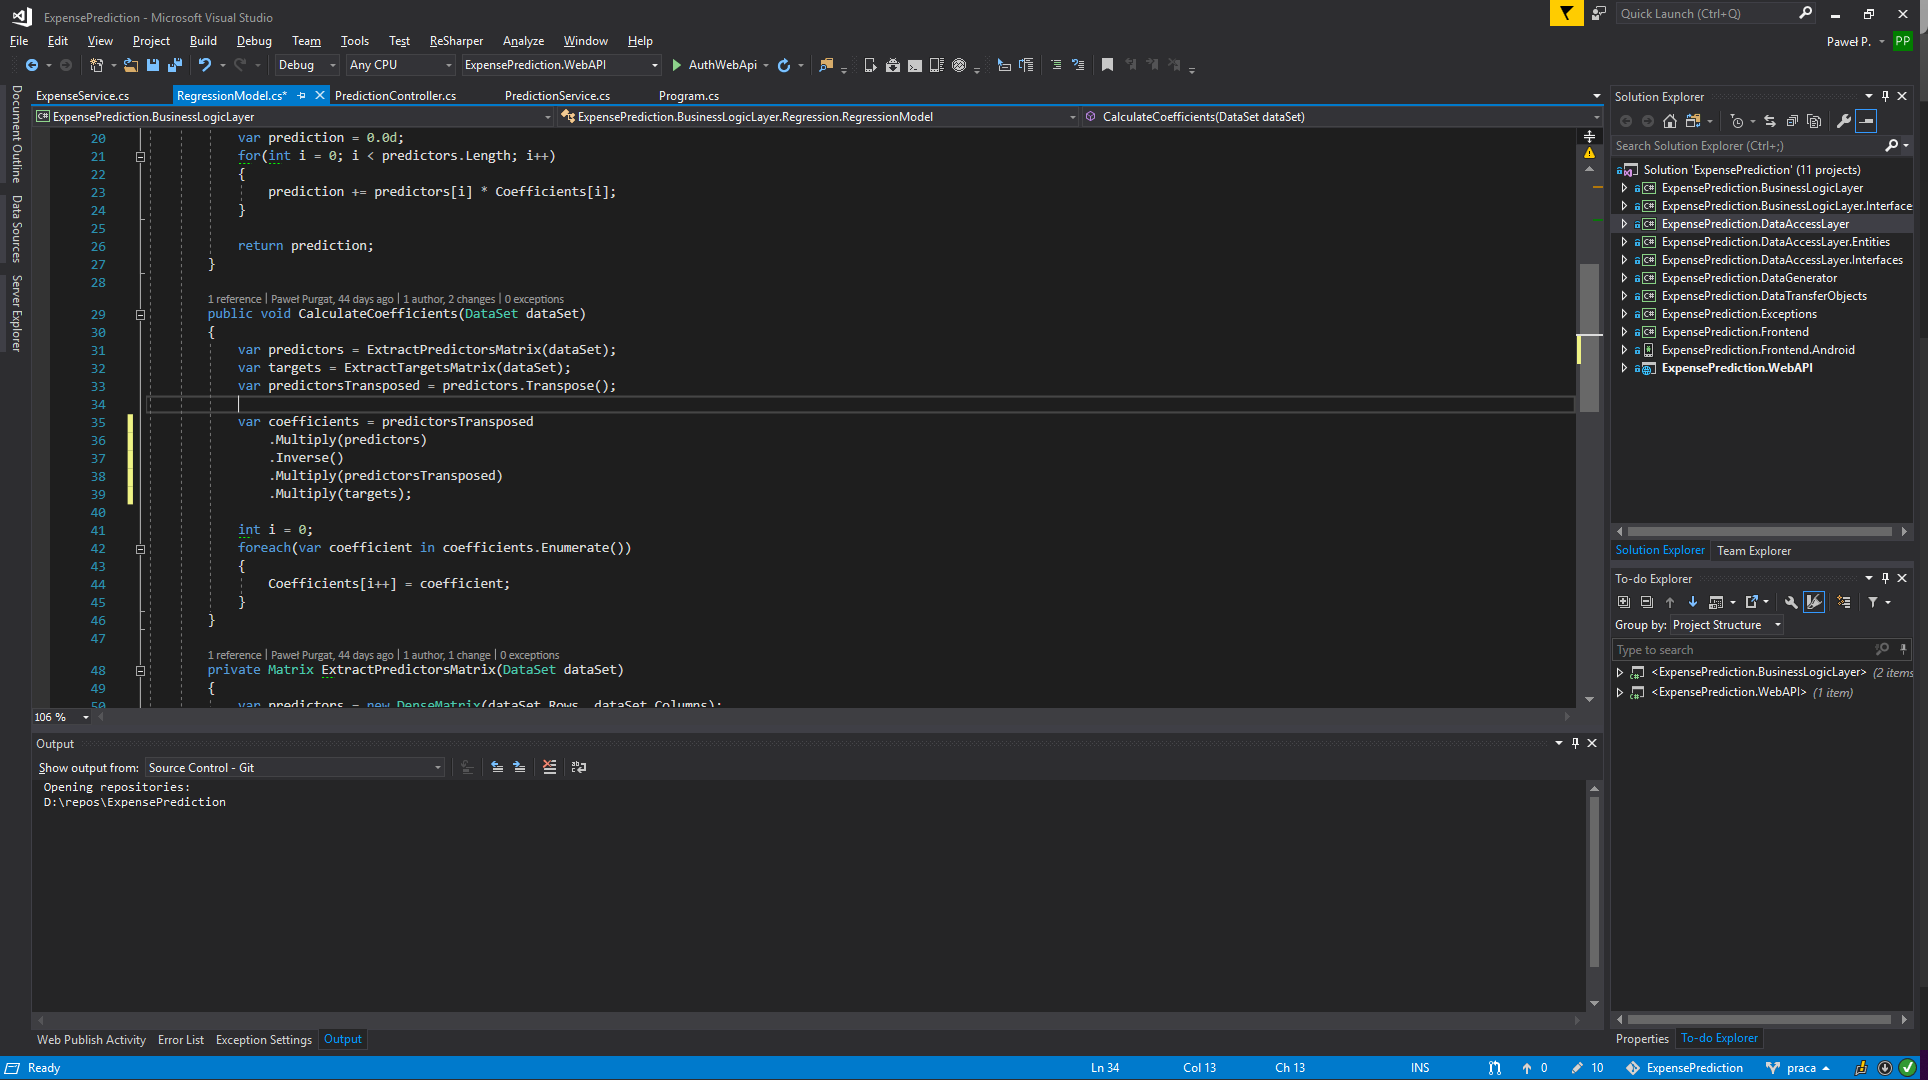
\includegraphics[width=6in]{img/aplikacje/vs_interfejs.png}
		\caption{Interfejs środowiska Microsoft Visual Studio}
		\label{vs_interfejs}
	\end{center}
\end{figure}

\textbf{ReSharper} (rys. \ref{resharper_interfejs}) jest narzędziem rozszerzającym środowisko Microsoft Visual Studio autorstwa JestBrains. Usprawnia ono proces wytwarzania oprogramowania poprzez automatyzację wielu procesów związanych z pisaniem wysokiej jakości kodu. Zapewnia ciągłą analizę kodu, co ułatwia wykrycie wielu błędów.\cite{resharper}
\begin{figure}[!ht]
	\begin{center}
		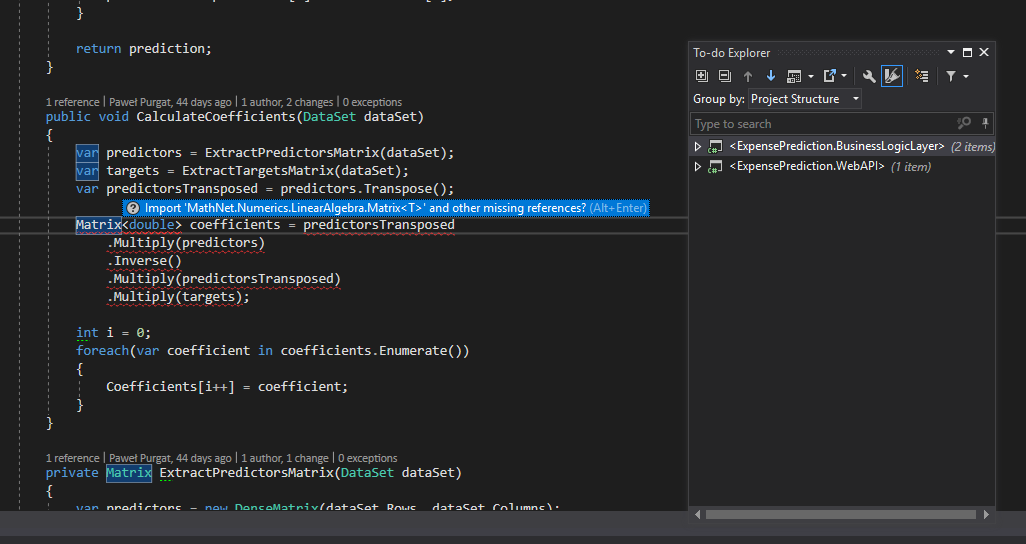
\includegraphics[width=6in]{img/aplikacje/resharper_interfejs.png}
		\caption{Przykładowe funkcjonalności rozszerzenia ReSharper}
		\label{resharper_interfejs}
	\end{center}
\end{figure}

\textbf{Postman} to aplikacja zapewniająca interfejs użytkownika służący do tworzenia i wysyłania zapytań do aplikacji internetowej. Zawiera ona kompleksowe narzędzia umożliwiające przegląd i analizę zapytań HTTP. \cite{postman}
\begin{figure}[!ht]
	\begin{center}
		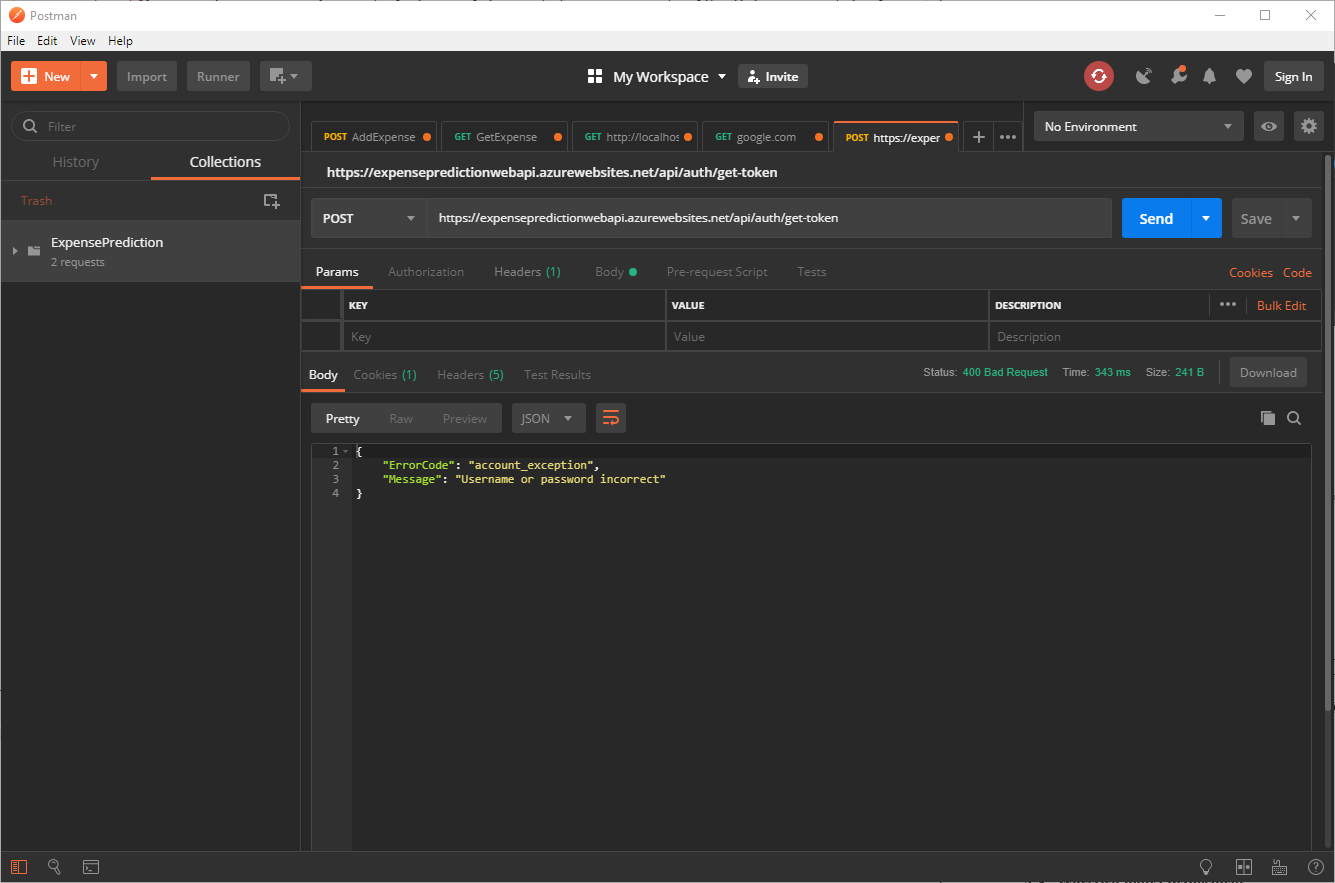
\includegraphics[width=6in]{img/aplikacje/postman_interfejs.png}
		\caption{Interfejs aplikacji Postman}
		\label{postman_interfejs}
	\end{center}
\end{figure}

\textbf{Swagger} (rys. \ref{swagger_interfejs}) jest narzędziem służącym do automatycznej dokumentacji kodu oraz zapewniającym konfigurowalny graficzny interfejs obrazujący stworzone API. Z poziomu wygenerowanego interfejsu możliwe jest proste konstruowanie zapytań zgodnych ze stworzoną aplikacją.\cite{swagger}
\begin{figure}[!ht]
	\begin{center}
		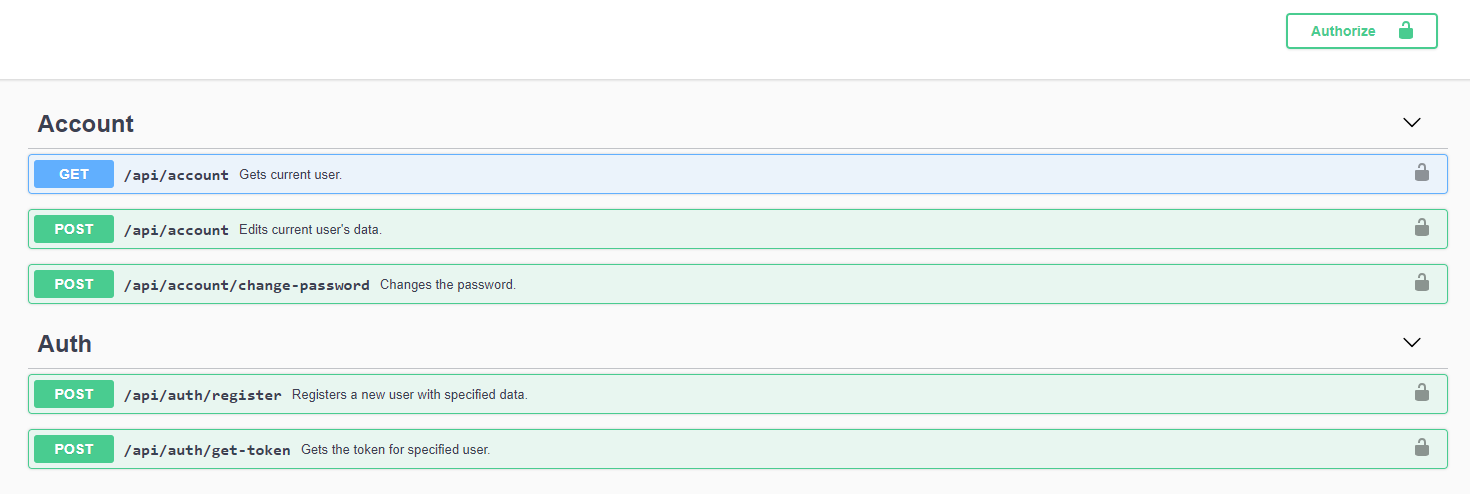
\includegraphics[width=6in]{img/aplikacje/swagger_interfejs.png}
		\caption{Interfejs wygenerowany przy użyciu narzędzia Swagger}
		\label{swagger_interfejs}
	\end{center}
\end{figure}
\section{Biblioteki}
%tutaj cos o nugecie też napisać chbya

%TODO: MVC, REST, LIBRARIES, EF CORE, DEPENDENCY INJECTION, LINQ
\chapter{Dokumentacja techniczna aplikacji do zarządzania budżetem i predykcji wydatków}
\section{Opis założeń projektu aplikacji}
\section{Warstwa modelu danych}
\section{Warstwa logiki biznesowej}
\section{Warstwa interfejsu użytkownika - aplikacja mobilna}
\chapter{Dokumentacja użytkownika aplikacji ExpensePredictor}
W niniejszym rozdziale opisany został interfejs użytkownika oraz funkcjonalność systemu ExpensePredictor. Diagram wszystkich przypadków użycia przedstawiony jest na Rys. \ref{usecases}.
\section{Moduł obsługi konta użytkownika}
Moduł obsługi konta użytkownika swoim zakresem obejmuje pięć przypadków użycia:
\begin{itemize}
	\item zarejestruj,
	\item zaloguj,
	\item wyświetl swoje dane,
	\item edytuj swoje dane,
	\item zmień swoje hasło.
\end{itemize}
\textbf{Rejestracja} (przypadek użycia "zarejestruj") to proces tworzenia nowego konta użytkownika. Jest jedną z dwóch funkcjonalności niewymagających uwierzytelnienia i dostępnych przy pierwszym uruchomieniu aplikacji. Po wybraniu na ekranie startowym (Rys. \ref{ekran_startowy_rejestracja}) przycisku "SIGN UP" otwarta zostaje strona rejestracji (Rys. \ref{rejestracja}). Po poprawnym wypełnieniu pól i naciśnięciu przycisku "SIGN UP" konto zostaje utworzone.
\begin{figure}[!ht]
	\begin{center}
		\begin{subfigure}[b]{0.3\textwidth}
				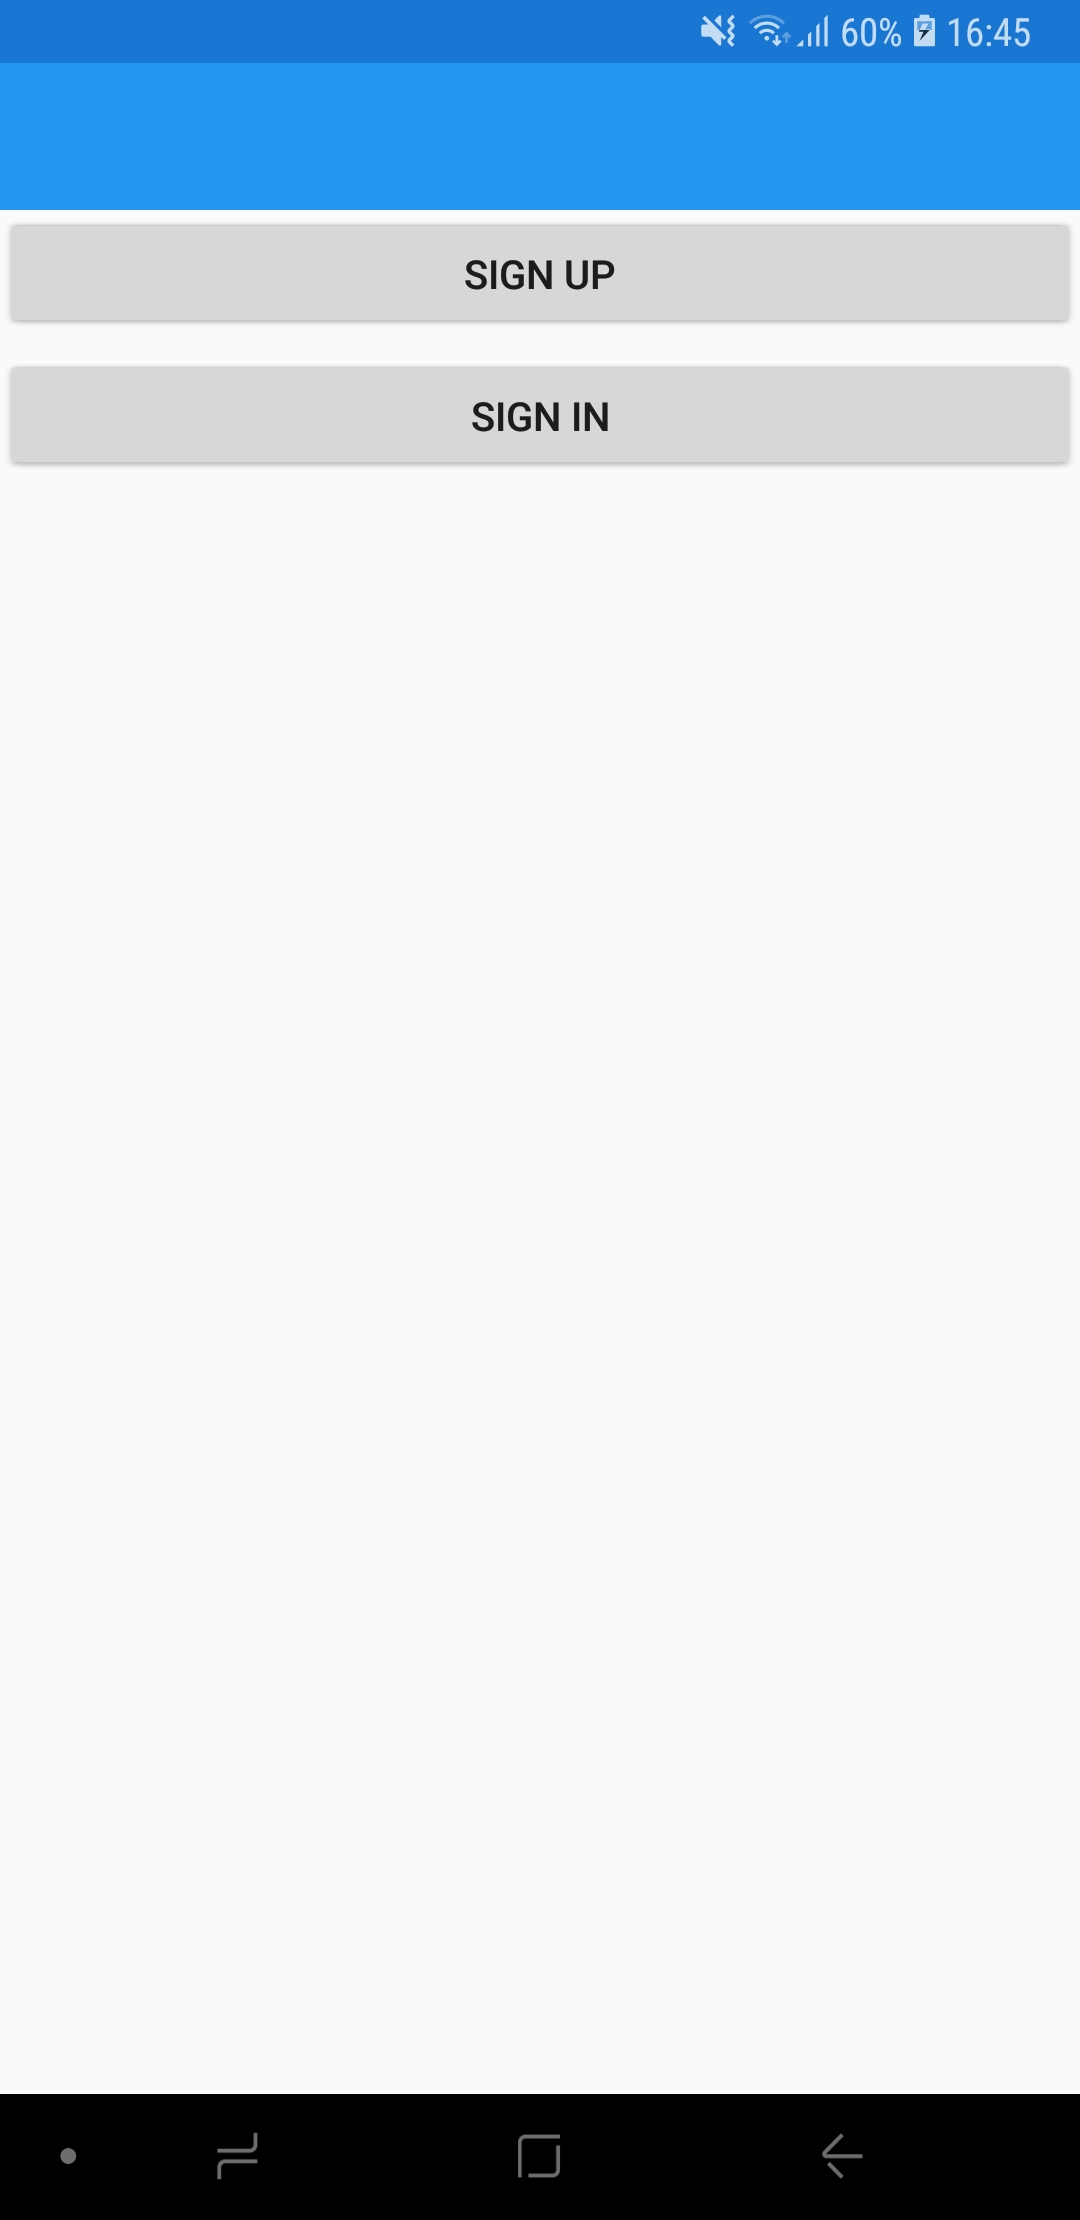
\includegraphics[width=1.75in]{img/mobile/ekran_startowy.jpg}
				\subcaption{Ekran startowy.}
				\label{ekran_startowy_rejestracja}
		\end{subfigure}
		\begin{subfigure}[b]{0.3\textwidth}
				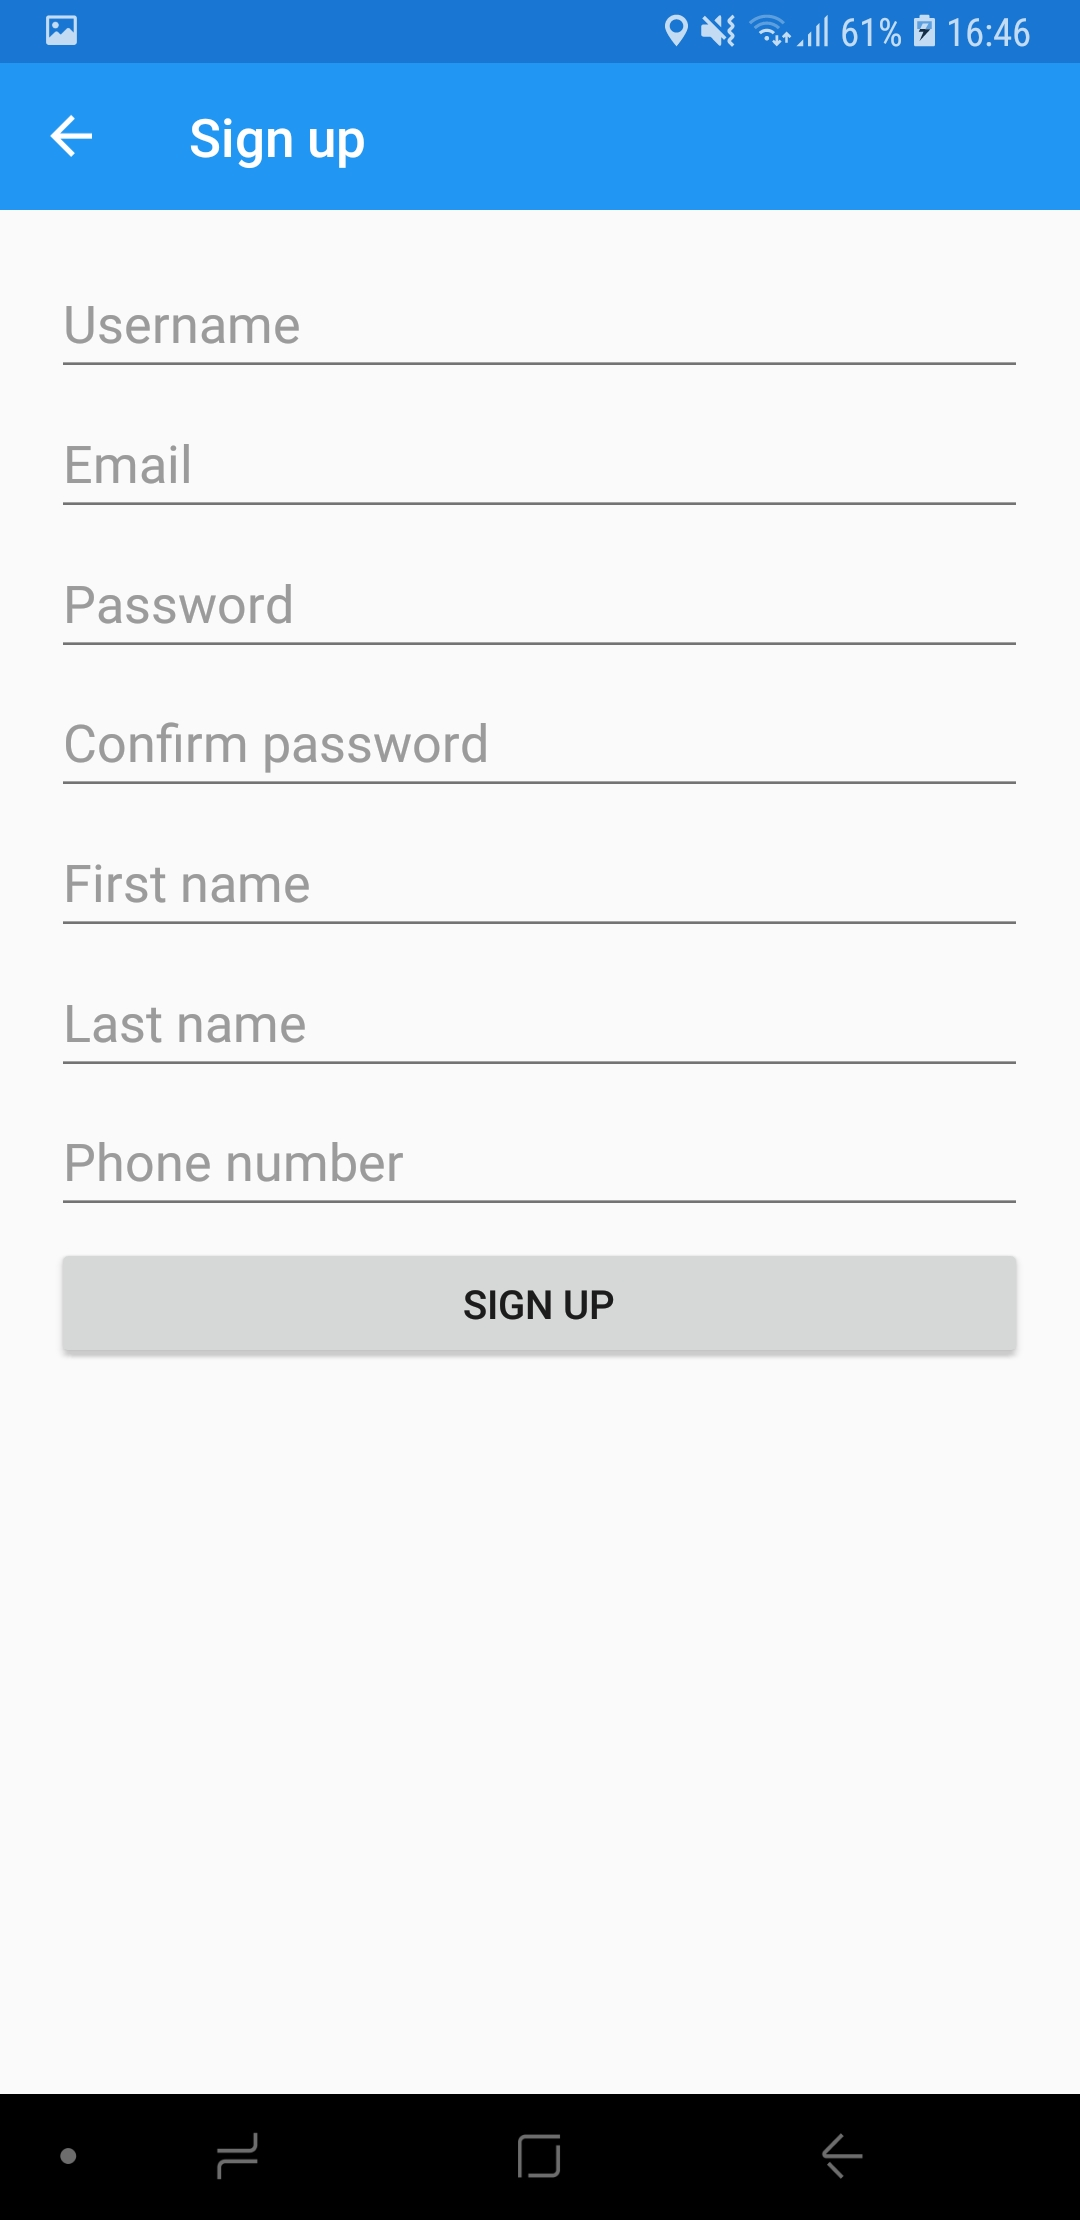
\includegraphics[width=1.75in]{img/mobile/rejestracja.jpg}
				\subcaption{Strona rejestracji.}
				\label{rejestracja}
		\end{subfigure}
	\end{center}
	\caption{Zrzuty ekranu procesu rejestracji.}
\end{figure}

\textbf{Logowanie} (przypadek użycia "zaloguj") jest procesem generacji tokenu uwierzytelniającego. Po wybraniu na ekranie startowym (Rys. \ref{ekran_startowy_logowanie}) przycisku "SIGN IN" wyświetla się strona logowania (Rys. \ref{logowanie}). Po wypełnieniu formularza i wciśnięciu przycisku "SIGN IN", w przypadku błędnego hasła wyświetla się komunikat (Rys. \ref{logowanie_haslo}), w przeciwnym wypadku proces kończy się powodzeniem.
\begin{figure}[!ht]
	\begin{center}
		\begin{subfigure}[b]{0.3\textwidth}
			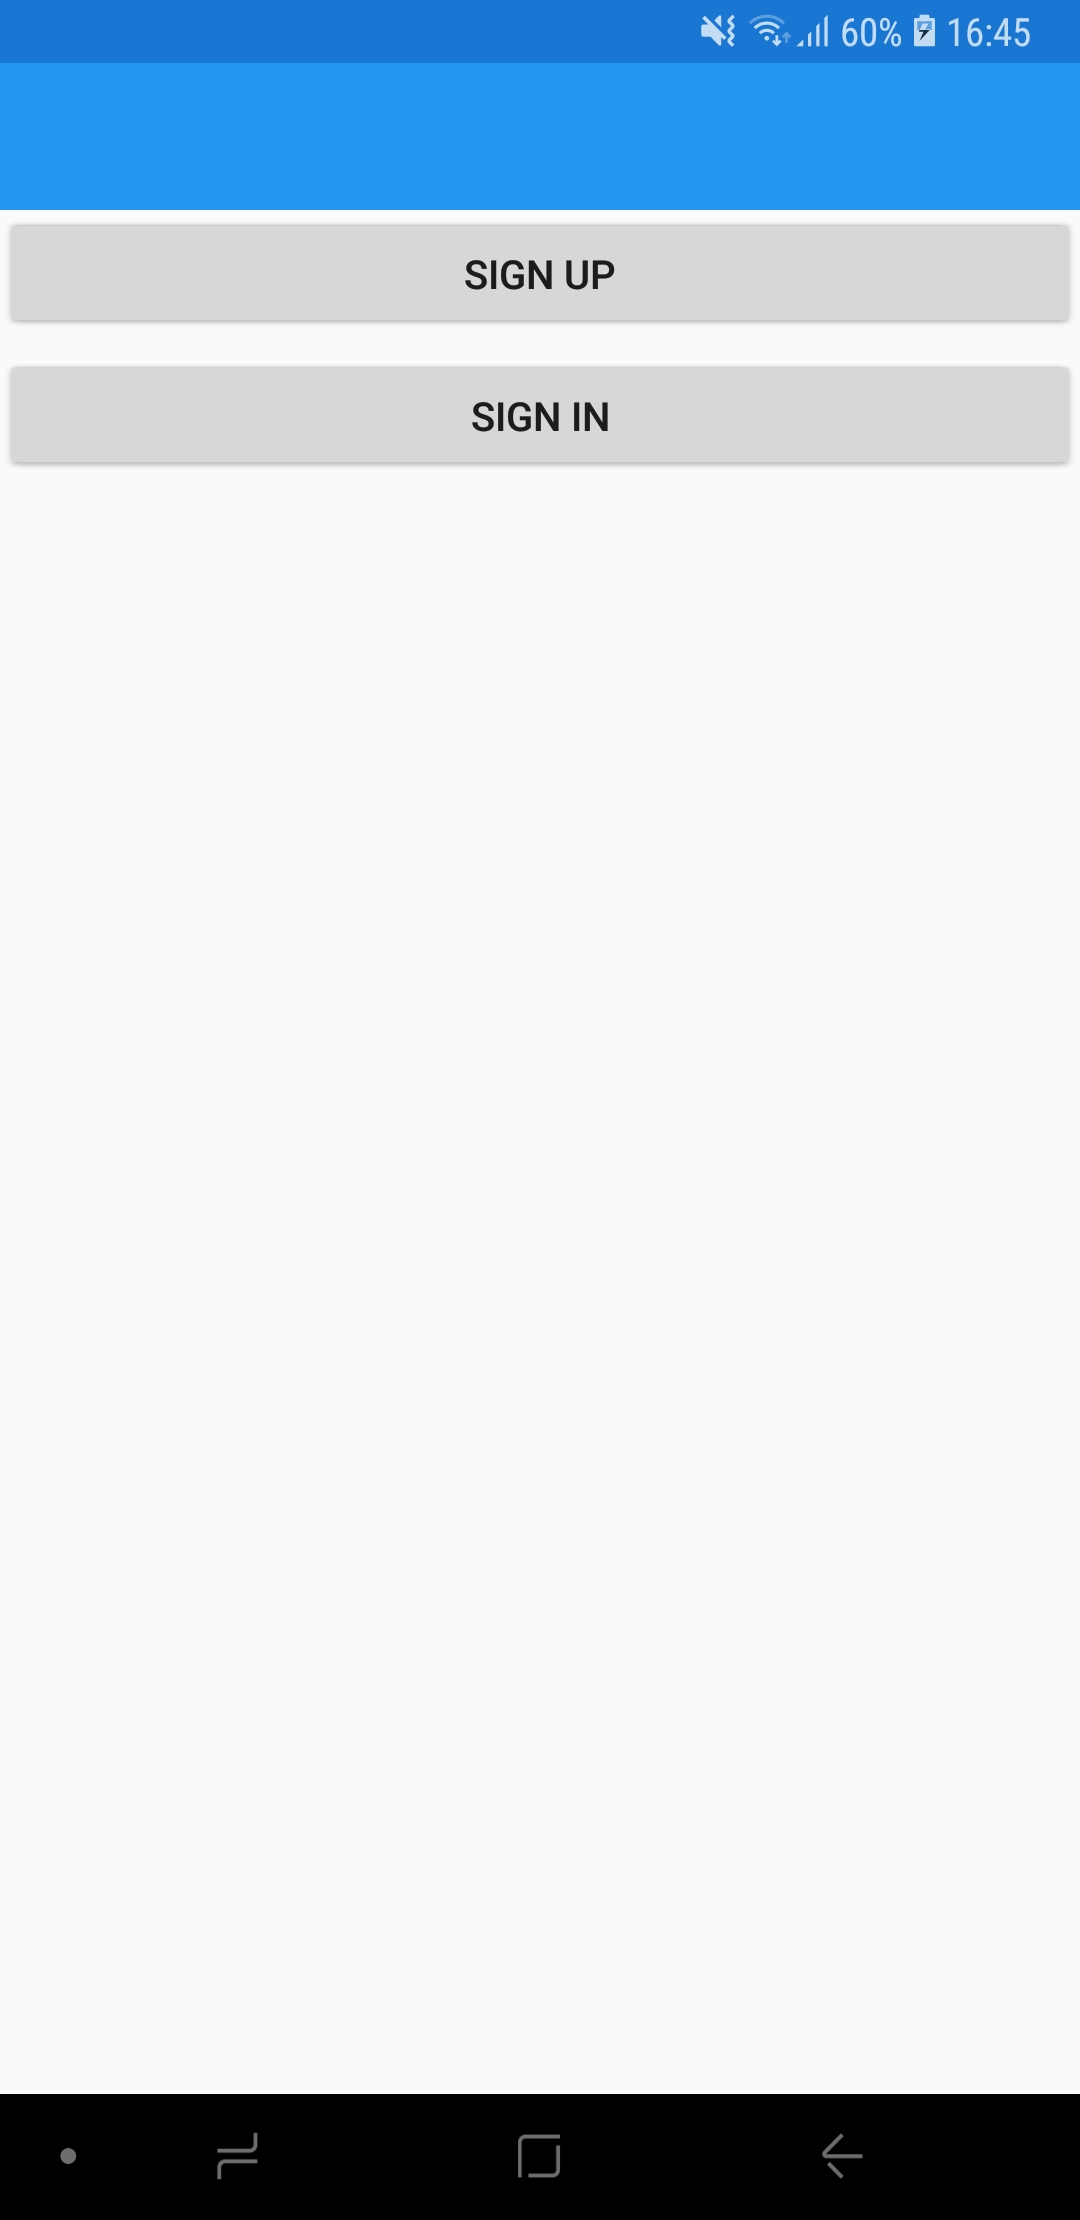
\includegraphics[width=1.75in]{img/mobile/ekran_startowy.jpg}
			\subcaption{Ekran startowy.}
			\label{ekran_startowy_logowanie}
		\end{subfigure}
		\begin{subfigure}[b]{0.3\textwidth}
			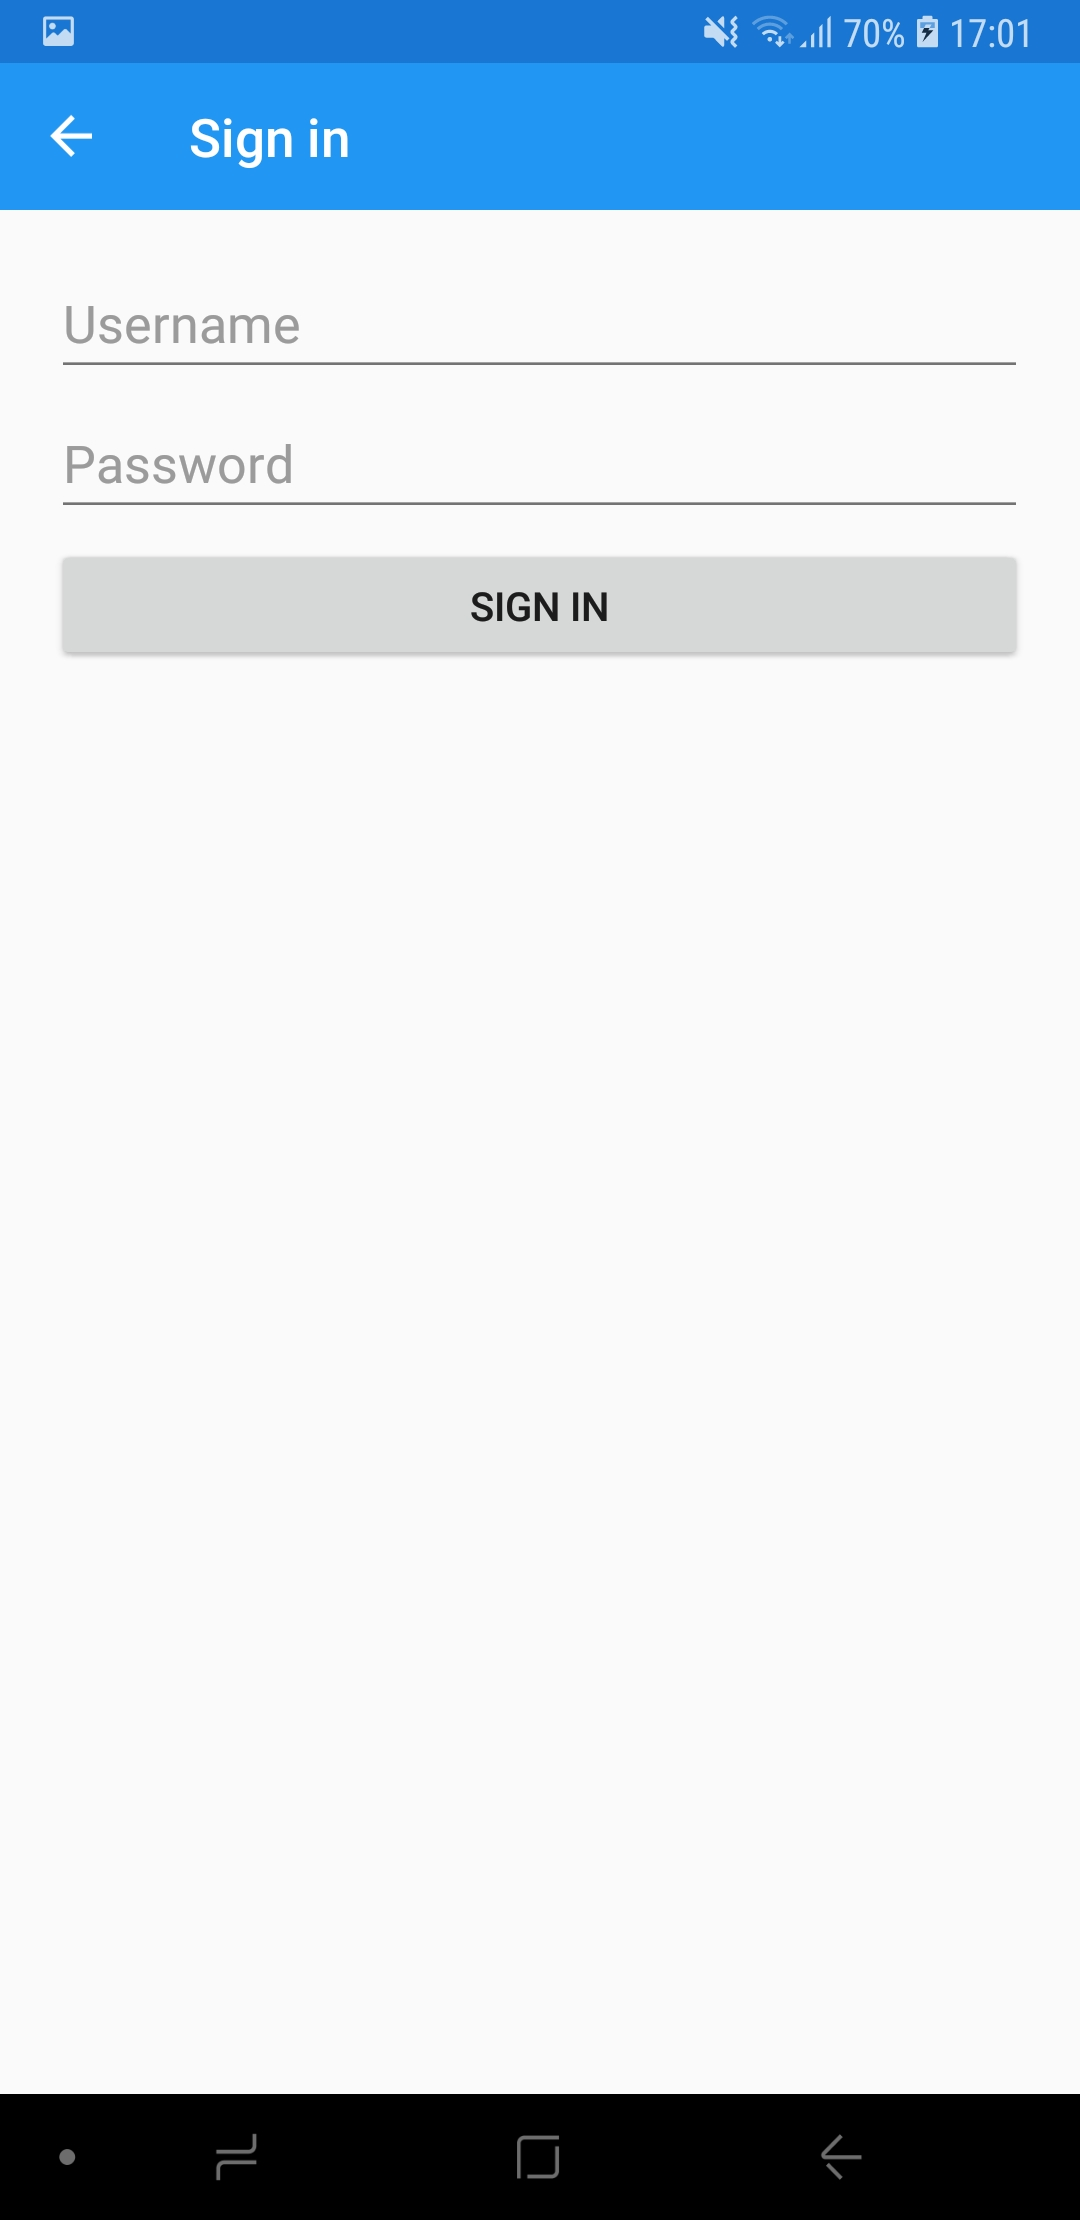
\includegraphics[width=1.75in]{img/mobile/login.jpg}
			\subcaption{Strona logowania.}
			\label{logowanie}
		\end{subfigure}
		\begin{subfigure}[b]{0.3\textwidth}
			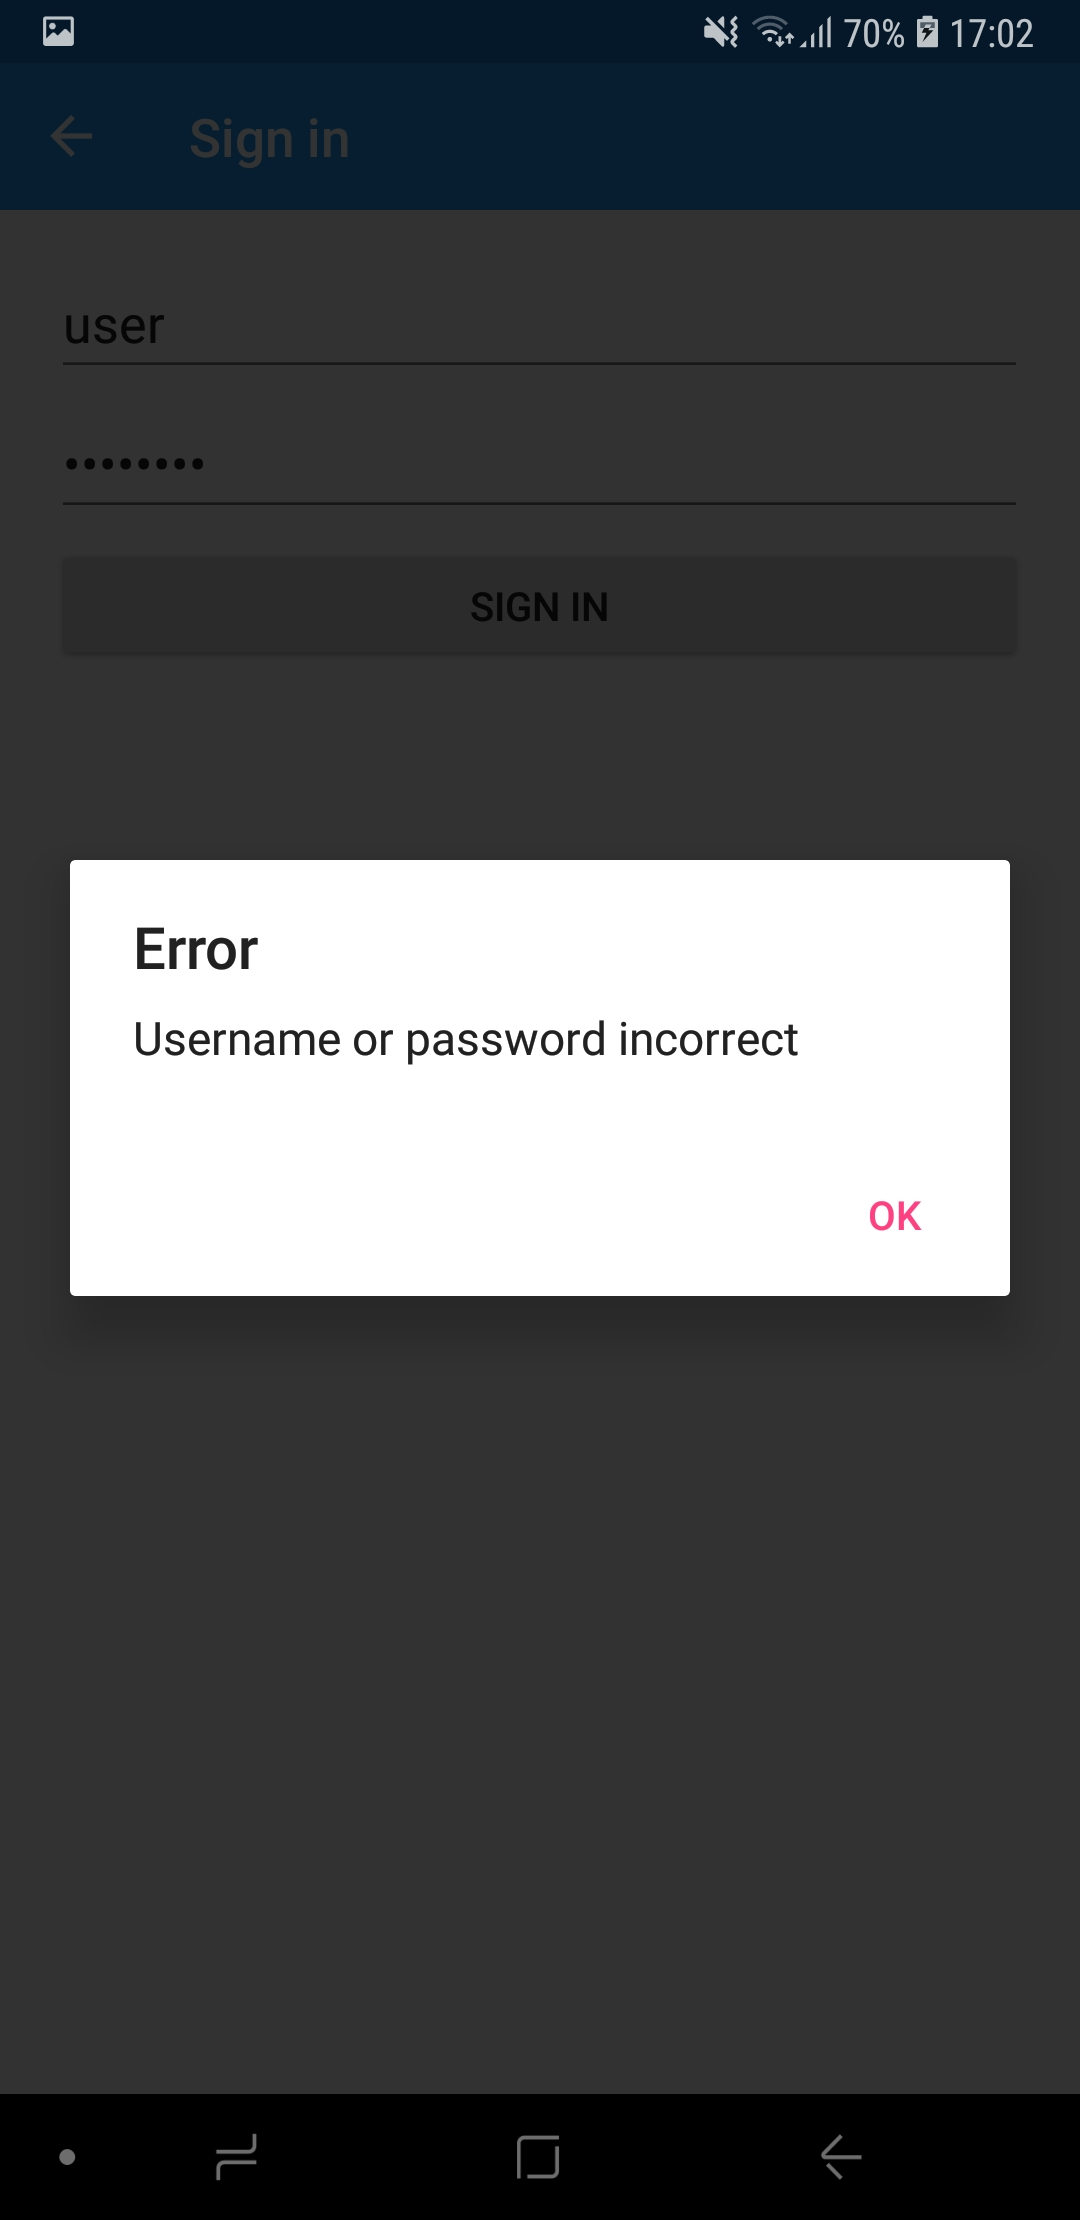
\includegraphics[width=1.75in]{img/mobile/logowanie_haslo.jpg}
			\subcaption{Błędne hasło.}
			\label{logowanie_haslo}
		\end{subfigure}
	\end{center}
	\caption{Zrzuty ekranu procesu logowania.}
\end{figure}

\textbf{Wyświetlanie danych użytkownika} (przypadek użycia "wyświetl swoje dane") - pobranie danych użytkownika i wyświetlenie ich użytkownikowi. Po uwierzytelnieniu się w aplikacji i wybraniu z menu bocznego strony "User details" (Rys. \ref{hamburger_uzytkownik}) użytkownikowi prezentowane są jego dane (Rys \ref{uzytkownik}).
\begin{figure}[!ht]
	\begin{center}
		\begin{subfigure}[b]{0.3\textwidth}
			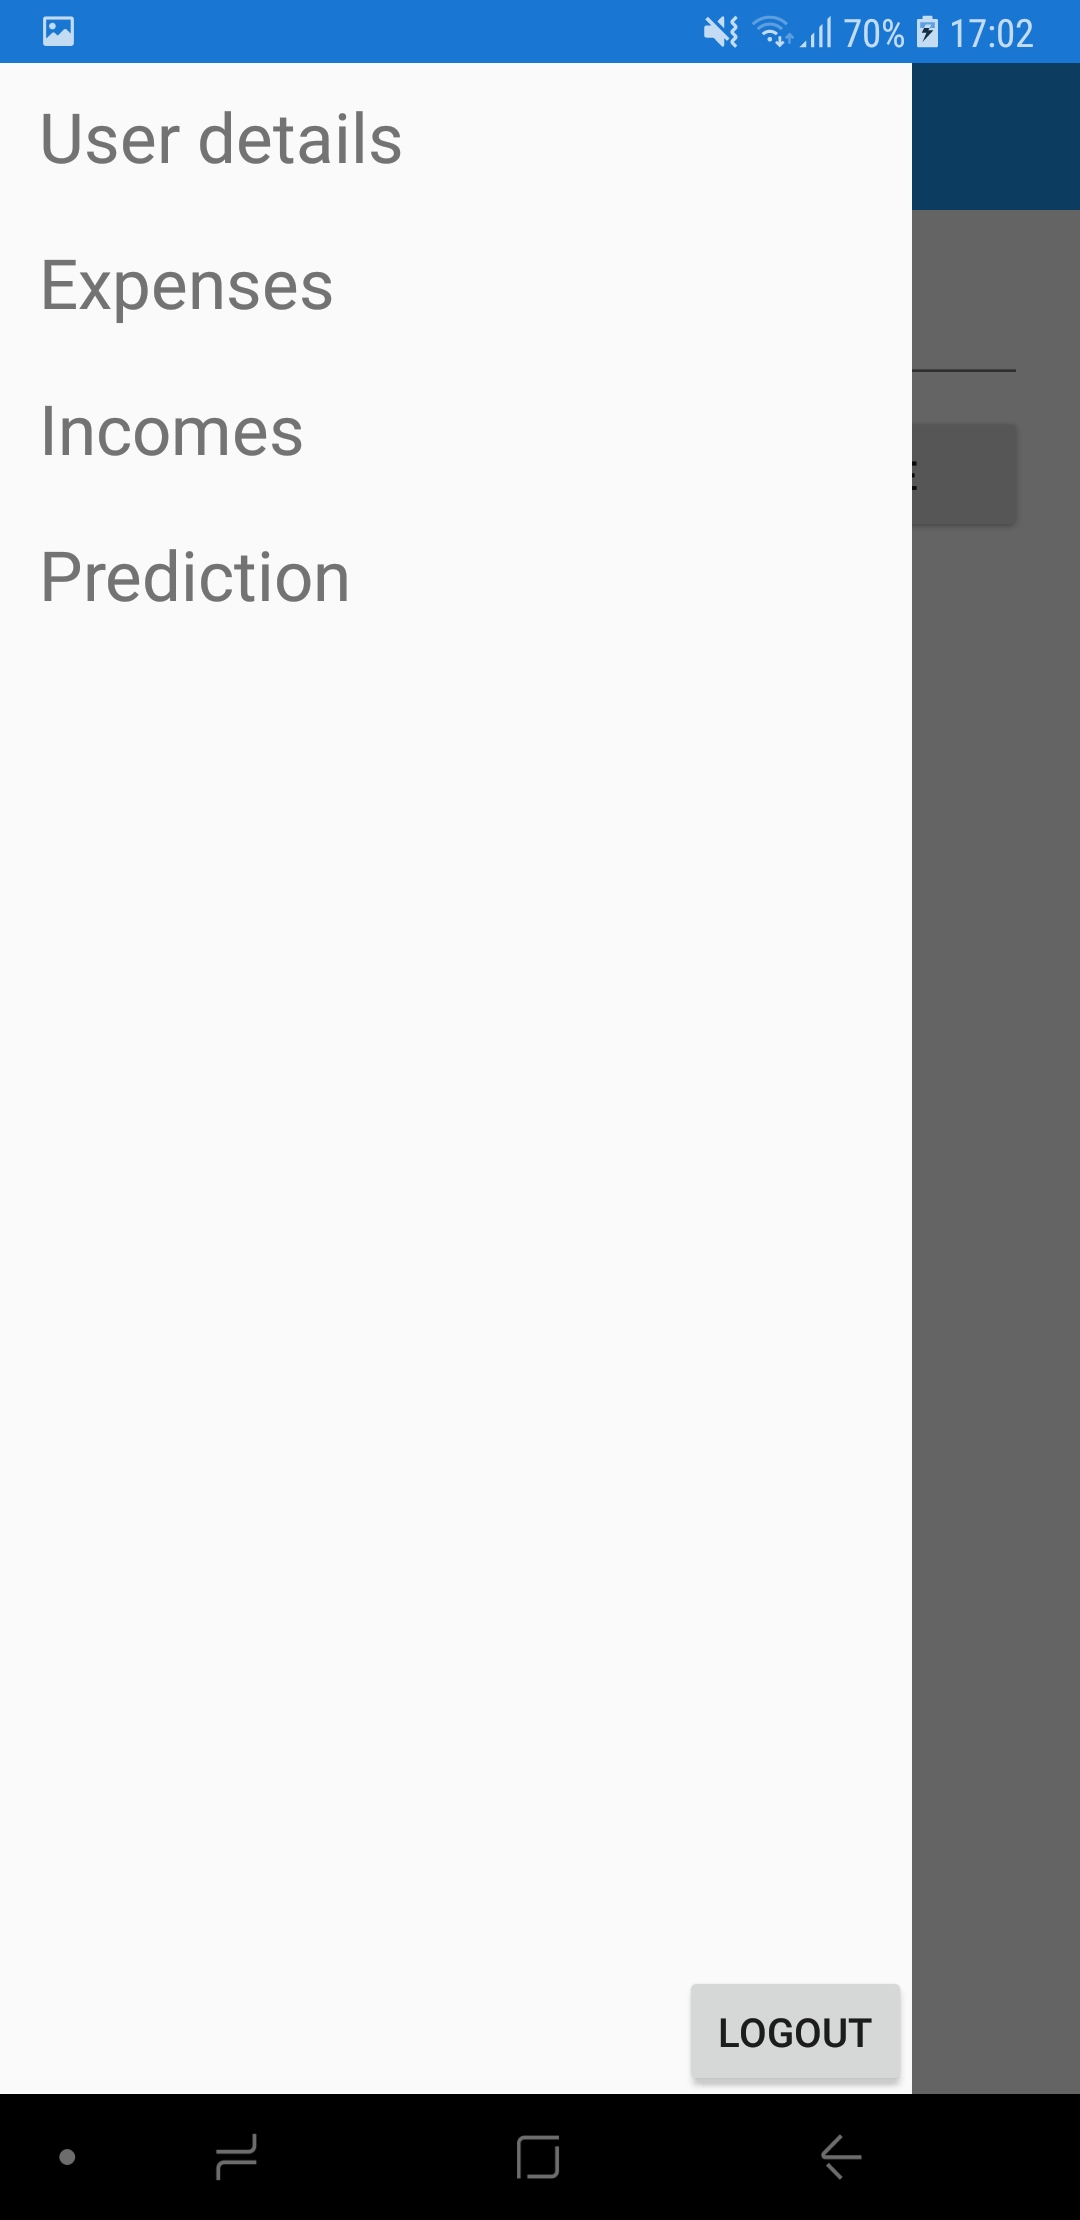
\includegraphics[width=1.75in]{img/mobile/menu_boczne.jpg}
			\subcaption{Menu boczne.}
			\label{hamburger_uzytkownik}
		\end{subfigure}
		\begin{subfigure}[b]{0.3\textwidth}
			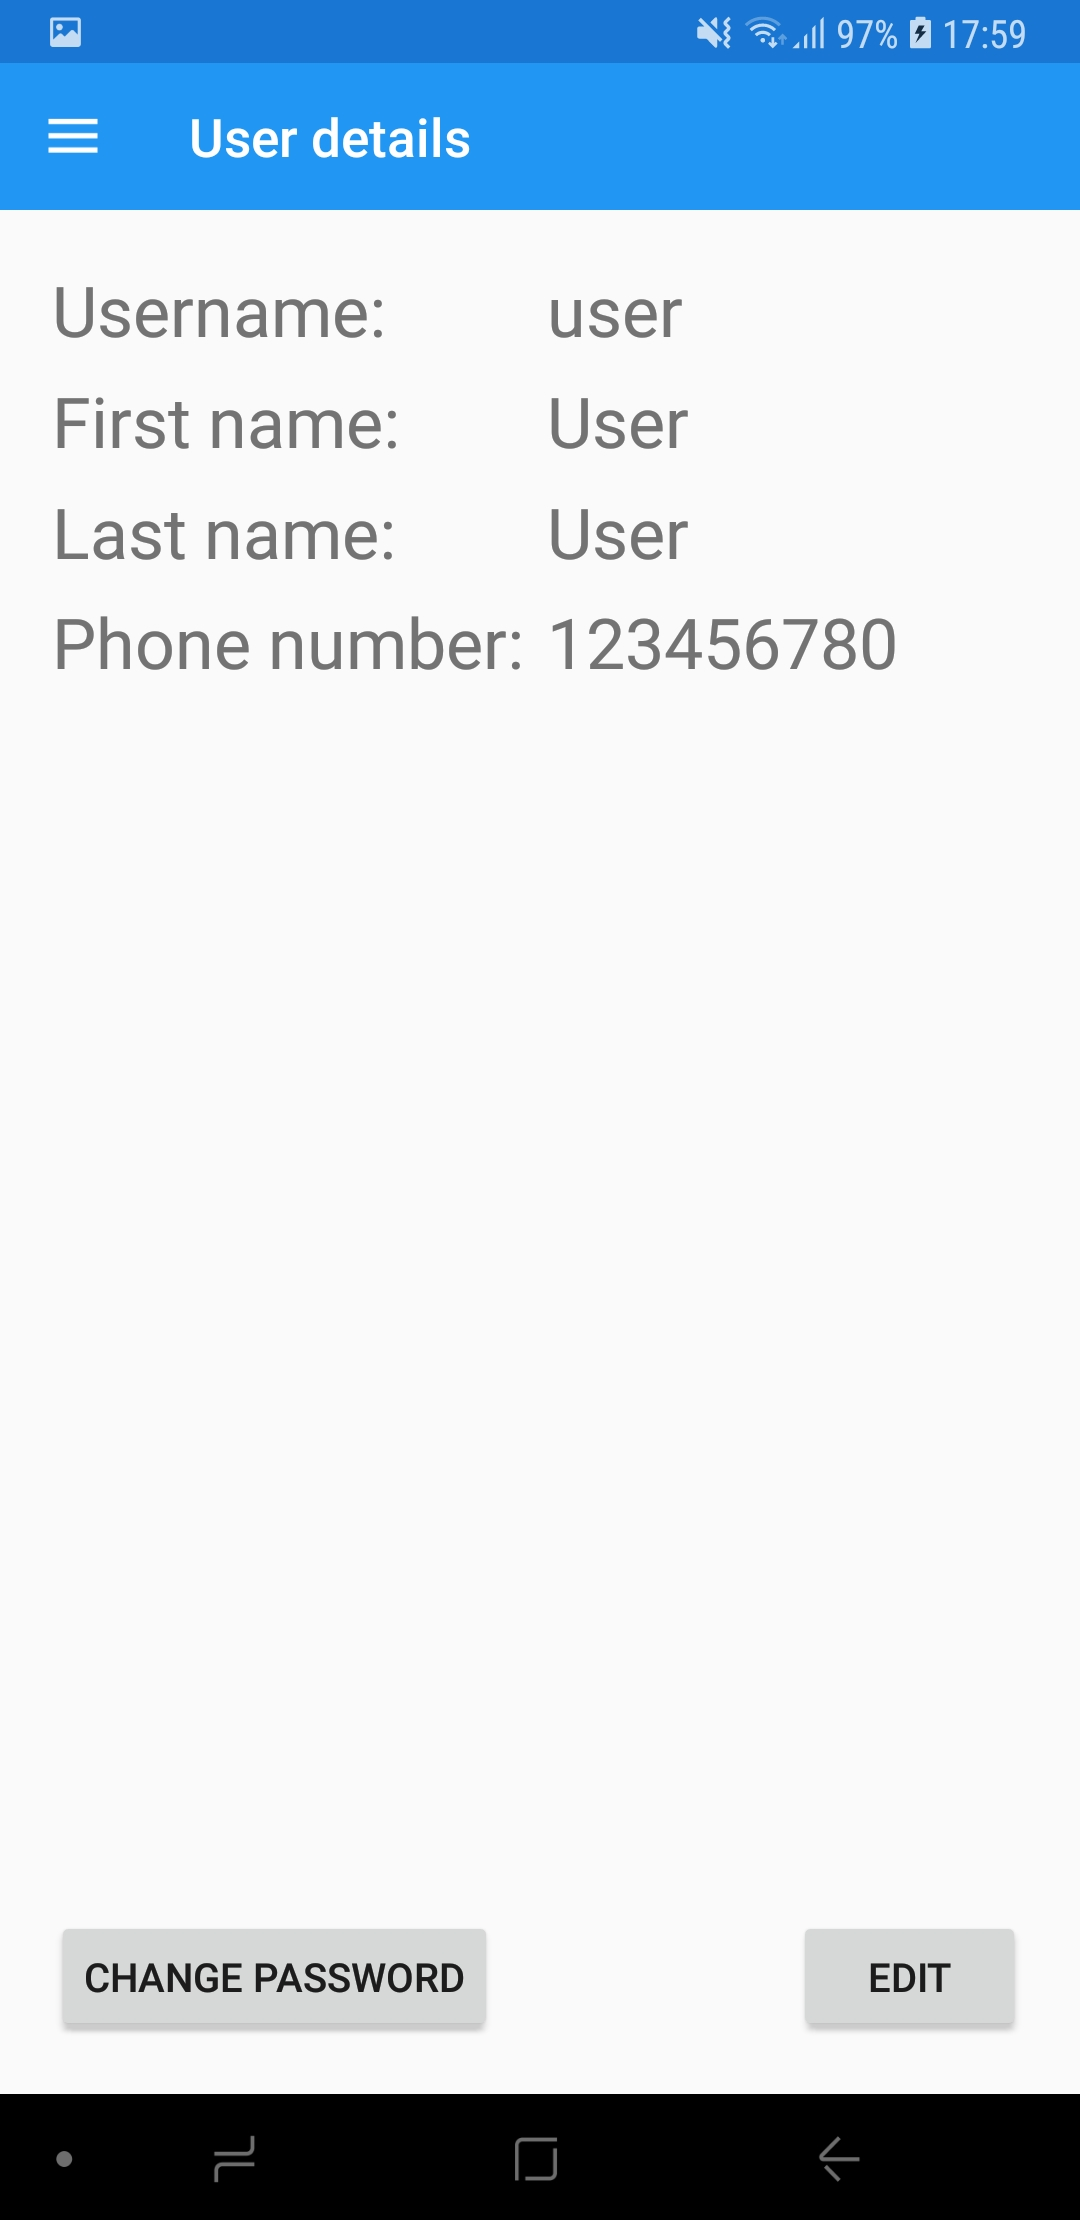
\includegraphics[width=1.75in]{img/mobile/uzytkownik.jpg}
			\subcaption{Dane użytkownika.}
			\label{uzytkownik}
		\end{subfigure}
	\end{center}
	\caption{Zrzuty ekranu procesu wyświetlania danych użytkownika.}
\end{figure}

\textbf{Edycja danych użytkownika} (przypadek użycia "edytuj swoje dane") - zmiana imienia, nazwiska bądź numeru telefonu użytkownika. Po przejściu na ekran danych użytkownika i wybraniu przycisku "EDIT" (Rys. \ref{uzytkownik_edit}) otwierany jest formularz edycji (Rys. \ref{edycja_uzytkownika}). Wciśnięcie przycisku "SUBMIT" edytuje dane użytkownika, przycisk "BACK" odrzuca wszelkie wprowadzone zmiany.
\begin{figure}[!ht]
	\begin{center}
		\begin{subfigure}[b]{0.3\textwidth}
			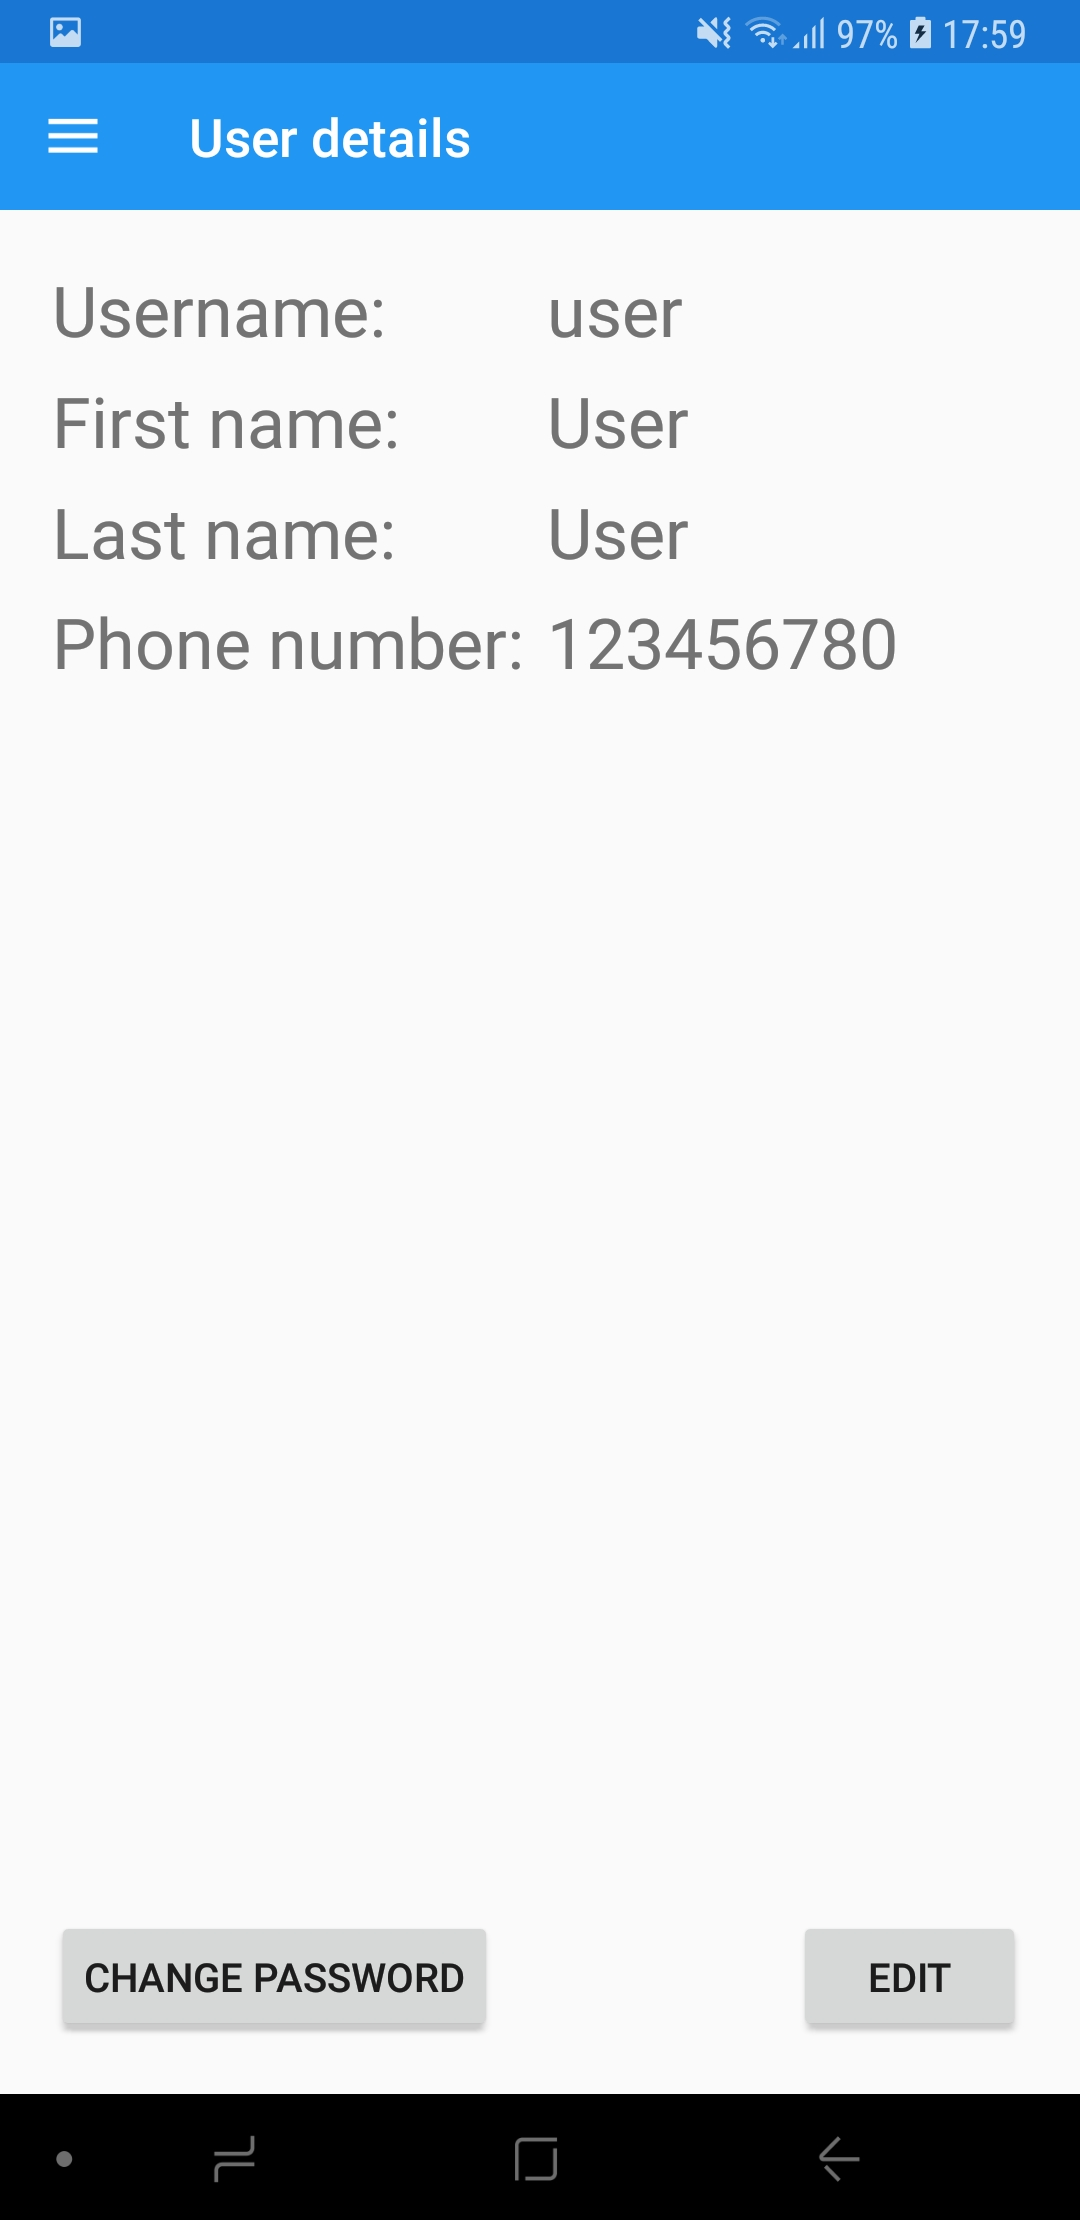
\includegraphics[width=1.75in]{img/mobile/uzytkownik.jpg}
			\subcaption{Dane użytkownika.\newline}
			\label{uzytkownik_edit}
		\end{subfigure}
		\begin{subfigure}[b]{0.3\textwidth}
			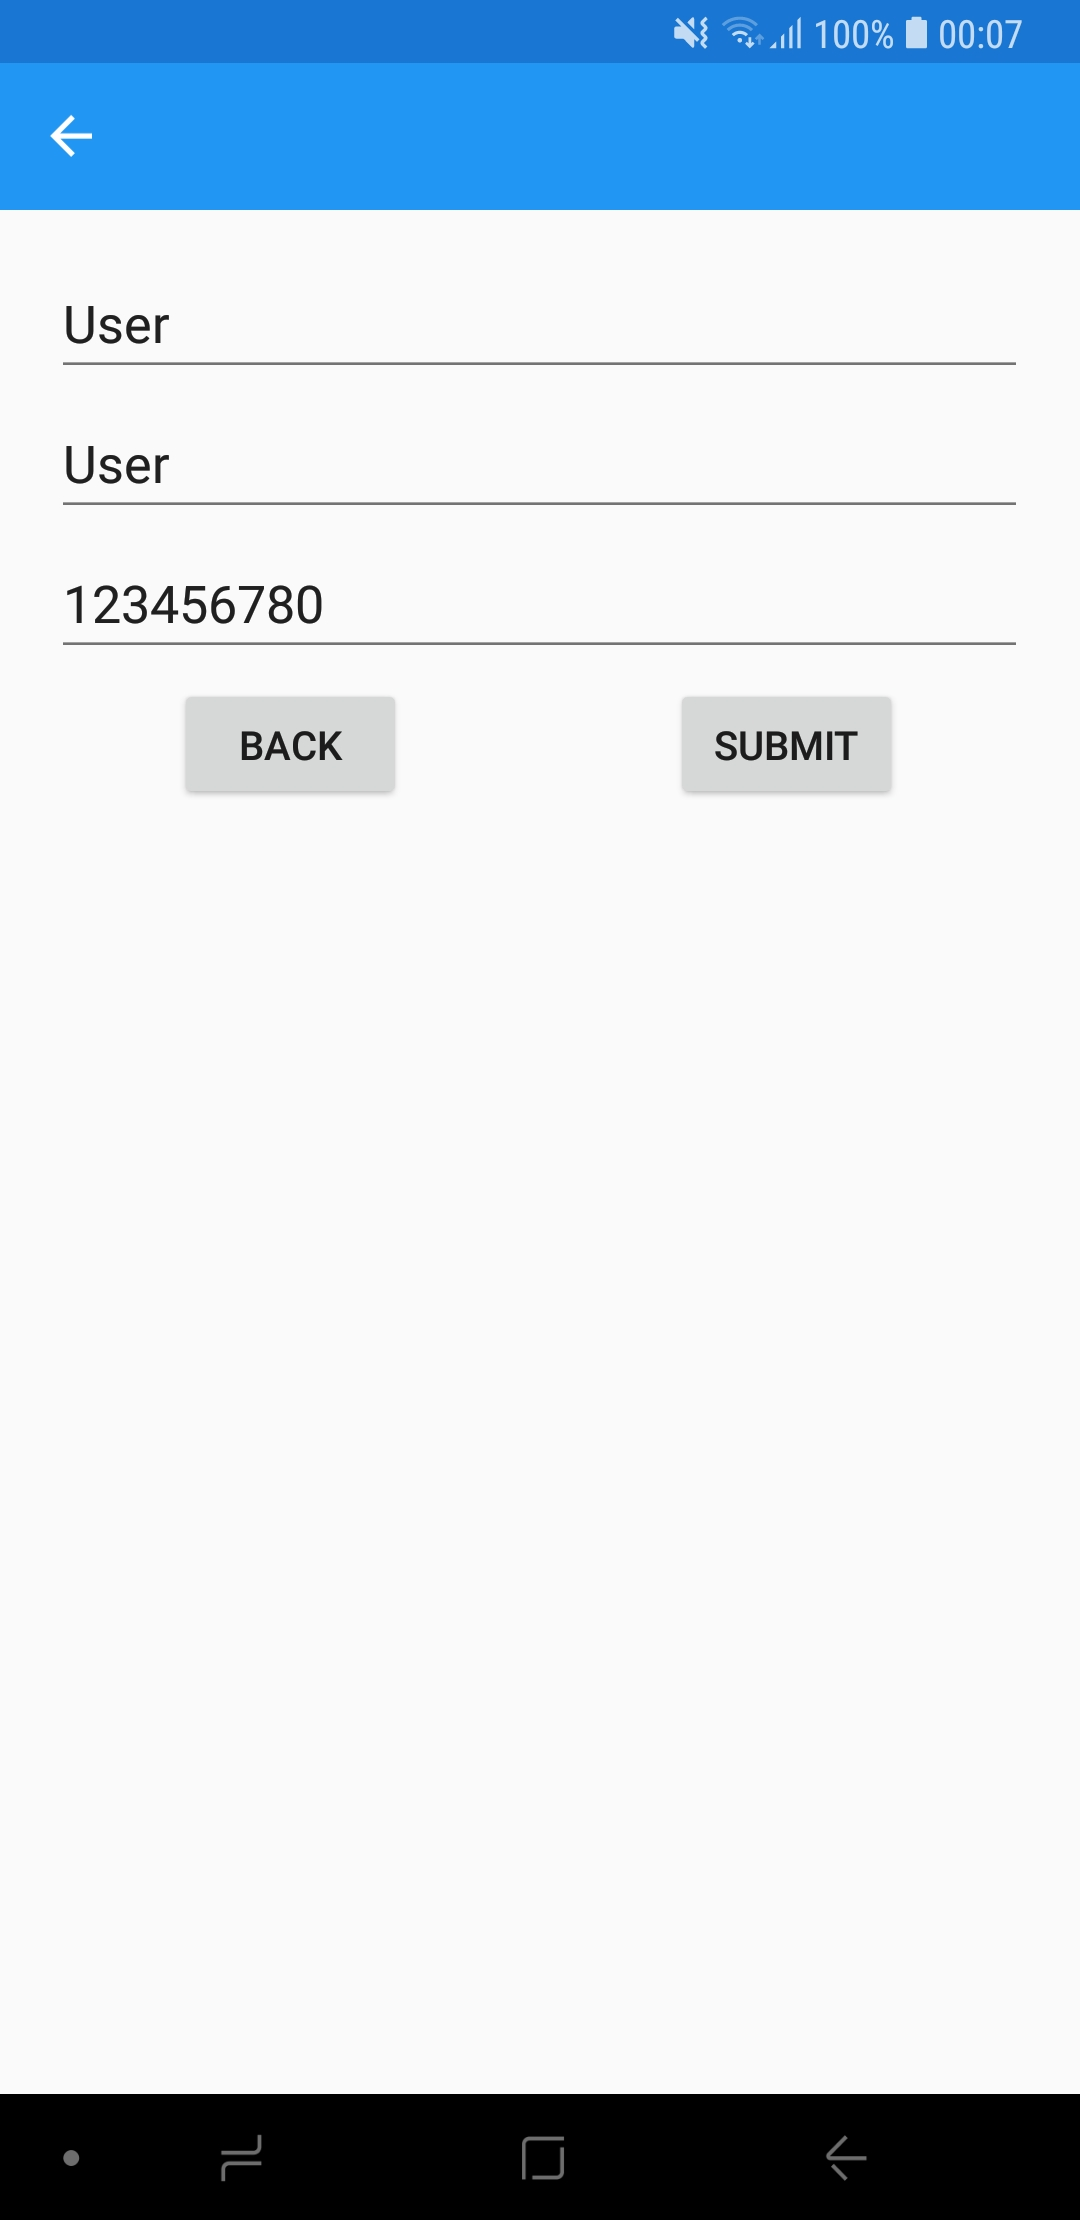
\includegraphics[width=1.75in]{img/mobile/edycja_uzytkownika.jpg}
			\subcaption{Edycja danych użytkownika.}
			\label{edycja_uzytkownika}
		\end{subfigure}
	\end{center}
	\caption{Zrzuty ekranu procesu edycji danych użytkownika.}
\end{figure}

\textbf{Zmiana hasła} (przypadek użycia "zmień swoje hasło) - ustawienie nowego hasła użytkownika. Po wybraniu przycisku "CHANGE PASSWORD" na ekranie danych użytkownika (Rys. \ref{uzytkownik_pass}) wyświetlany jest formularz zmiany hasła (Rys. \ref{haslo}). Poprawne wypełnienie formularza i naciśnięcie przycisku "SUBMIT" skutkuje zmianą hasła lub, jeżeli nie spełnia ono polityki haseł, wyświetlany jest komunikat o błędzie (Rys. \ref{haslo_blad}). Wciśnięcie przycisku "BACK" powoduje powrót do strony danych użytkownika.
\begin{figure}[!ht]
	\begin{center}
		\begin{subfigure}[b]{0.3\textwidth}
			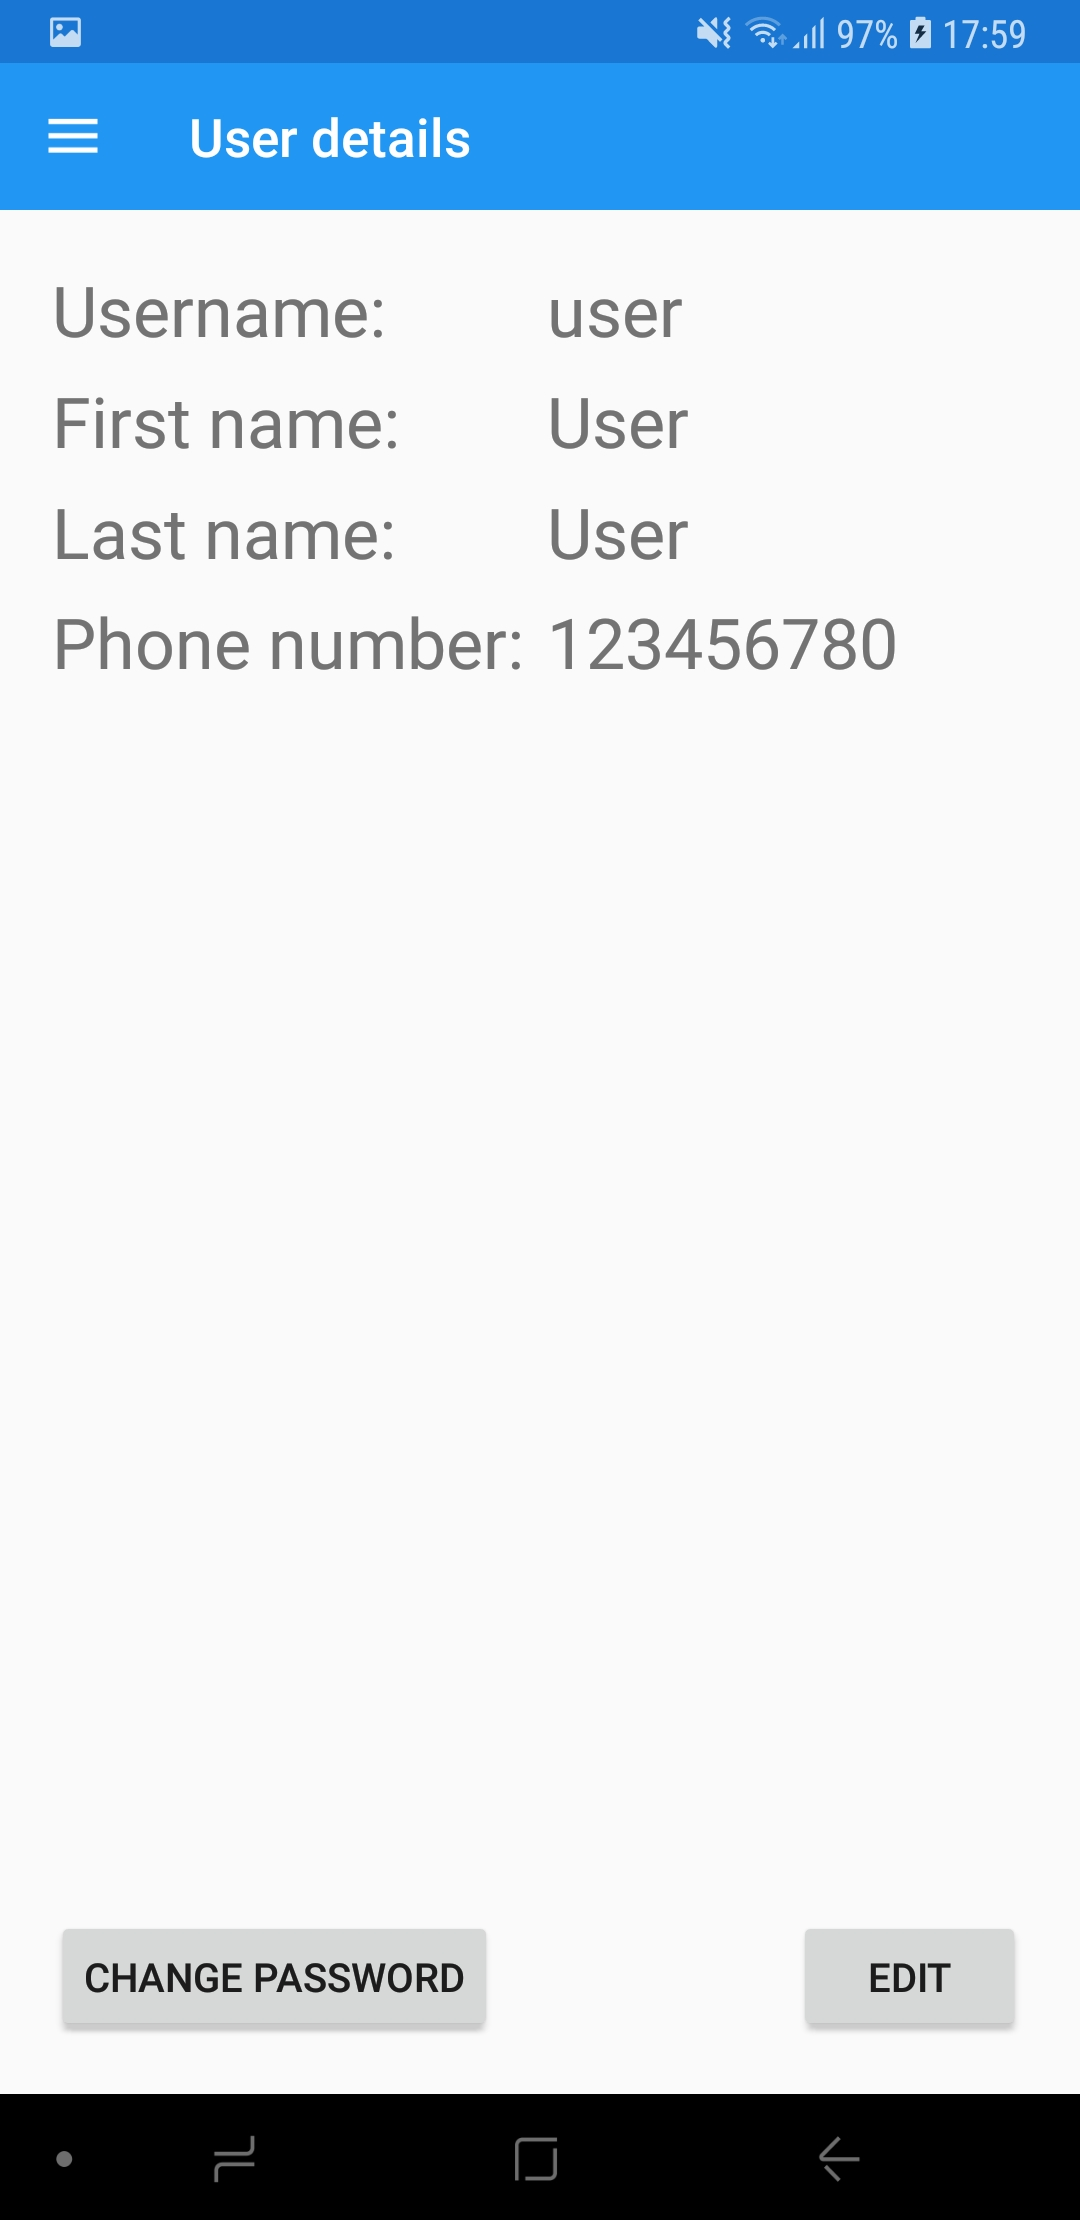
\includegraphics[width=1.75in]{img/mobile/uzytkownik.jpg}
			\subcaption{Dane użytkownika.}
			\label{uzytkownik_pass}
		\end{subfigure}
		\begin{subfigure}[b]{0.3\textwidth}
			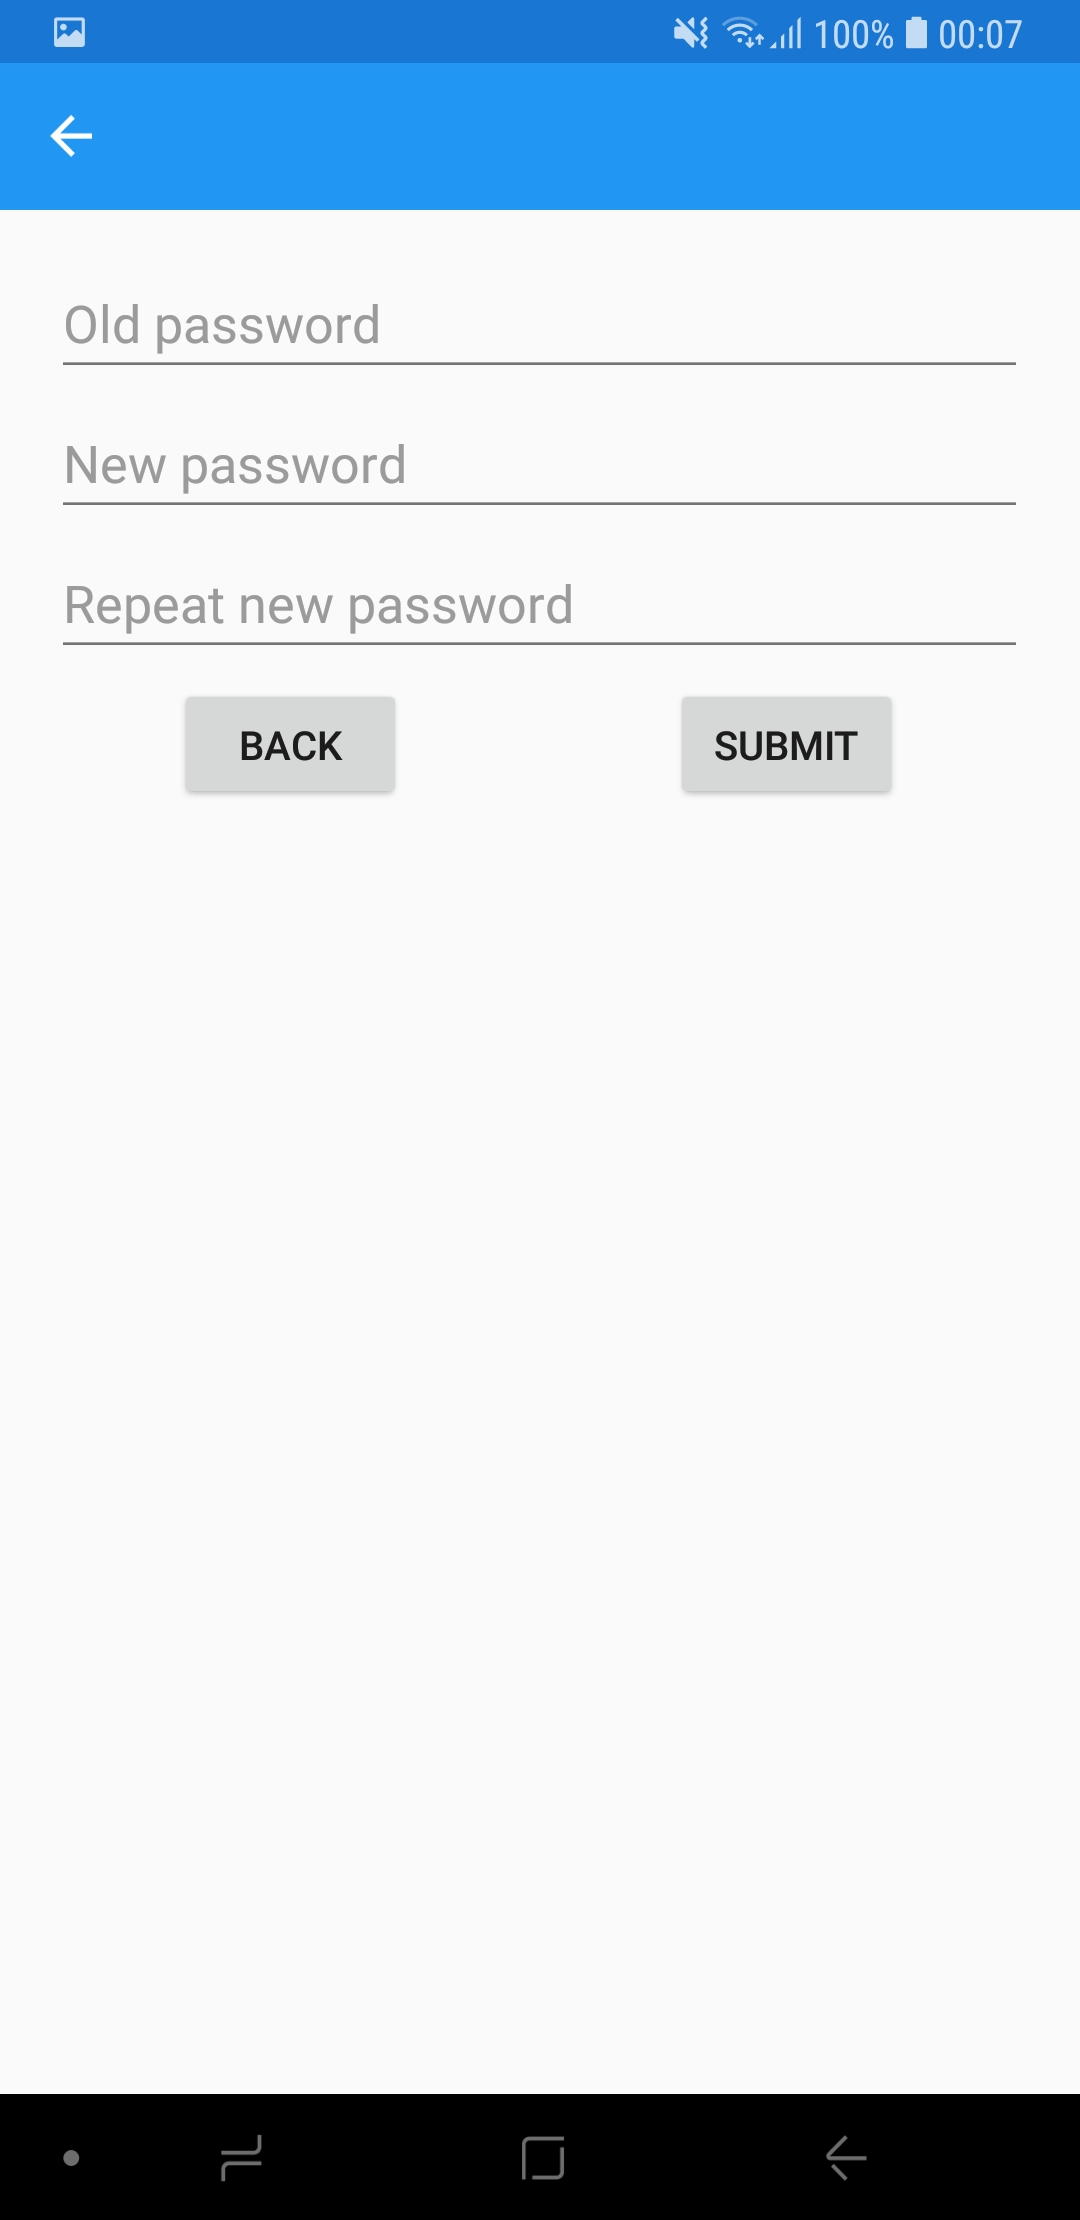
\includegraphics[width=1.75in]{img/mobile/haslo.jpg}
			\subcaption{Formularz zmiany hasła.}
			\label{haslo}
		\end{subfigure}
		\begin{subfigure}[b]{0.3\textwidth}
			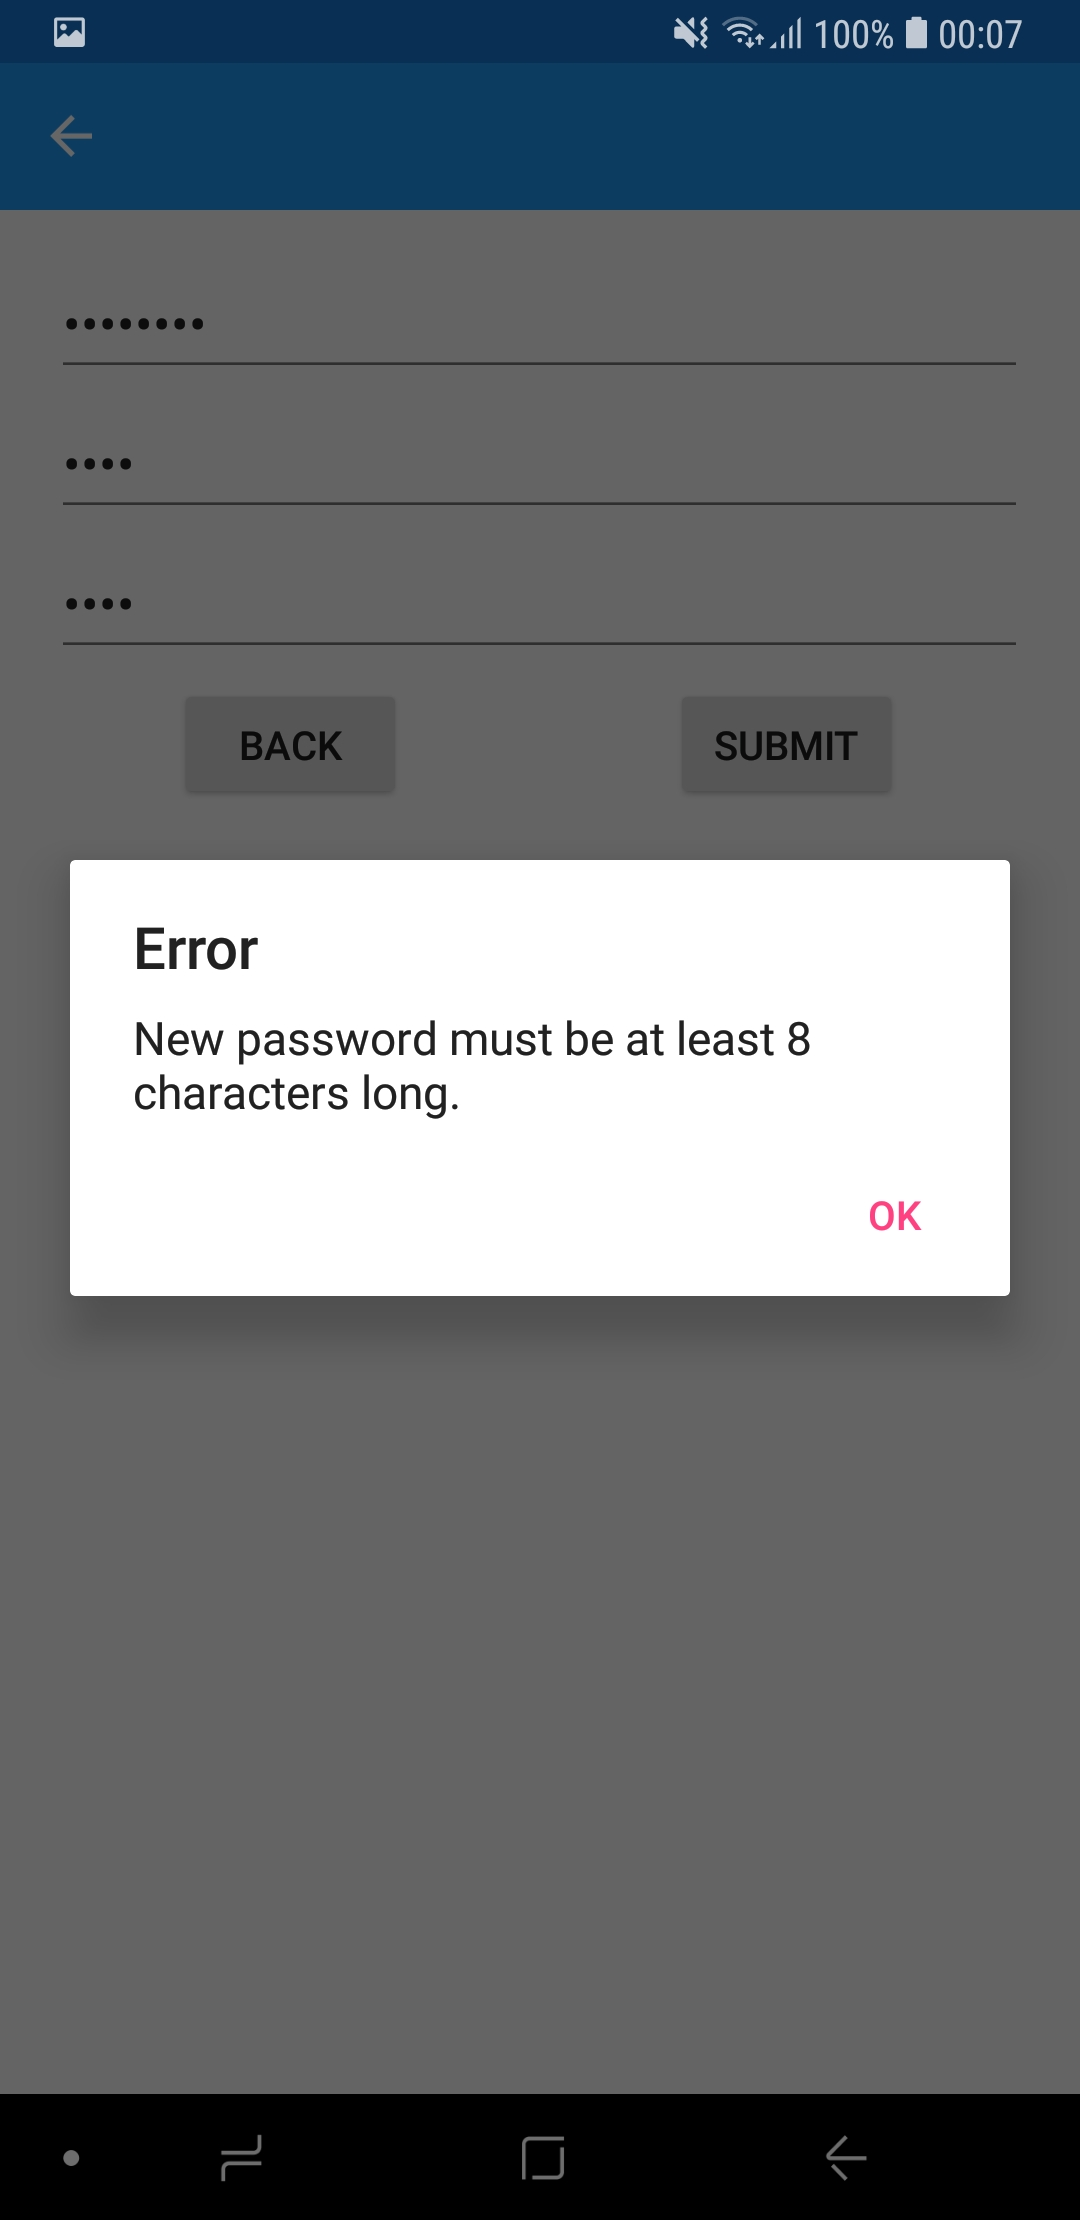
\includegraphics[width=1.75in]{img/mobile/haslo_blad.jpg}
			\subcaption{Komunikat o błędzie.}
			\label{haslo_blad}
		\end{subfigure}
	\end{center}
	\caption{Zrzuty ekranu procesu zmiany hasła.}
\end{figure}
\section{Moduł rejestracji przychodów}
Moduł rejestracji przychodów składa się z czterech przypadków użycia:
\begin{itemize}
\item wyświetl swoje przychody,
\item dodaj przychód,
\item edytuj przychód,
\item usuń przychód.
\end{itemize}

\textbf{Wyświetlanie przychodów} (przypadek użycia "wyświetl swoje przychody") - pobranie i zaprezentowanie użytkownikowi listy jego przychodów z danego okresu. Po wybraniu z menu bocznego (Rys. \ref{hamburger_przychody}) strony "Incomes" (Rys. \ref{przychody}), określeniu daty początkowej i końcowej oraz naciśnięciu przycisku "GET INCOMES" wyświetlana jest lista przychodów z wybranego okresu (Rys. \ref{przychody_gotowe}).
\begin{figure}[!ht]
	\begin{center}
		\begin{subfigure}[b]{0.3\textwidth}
			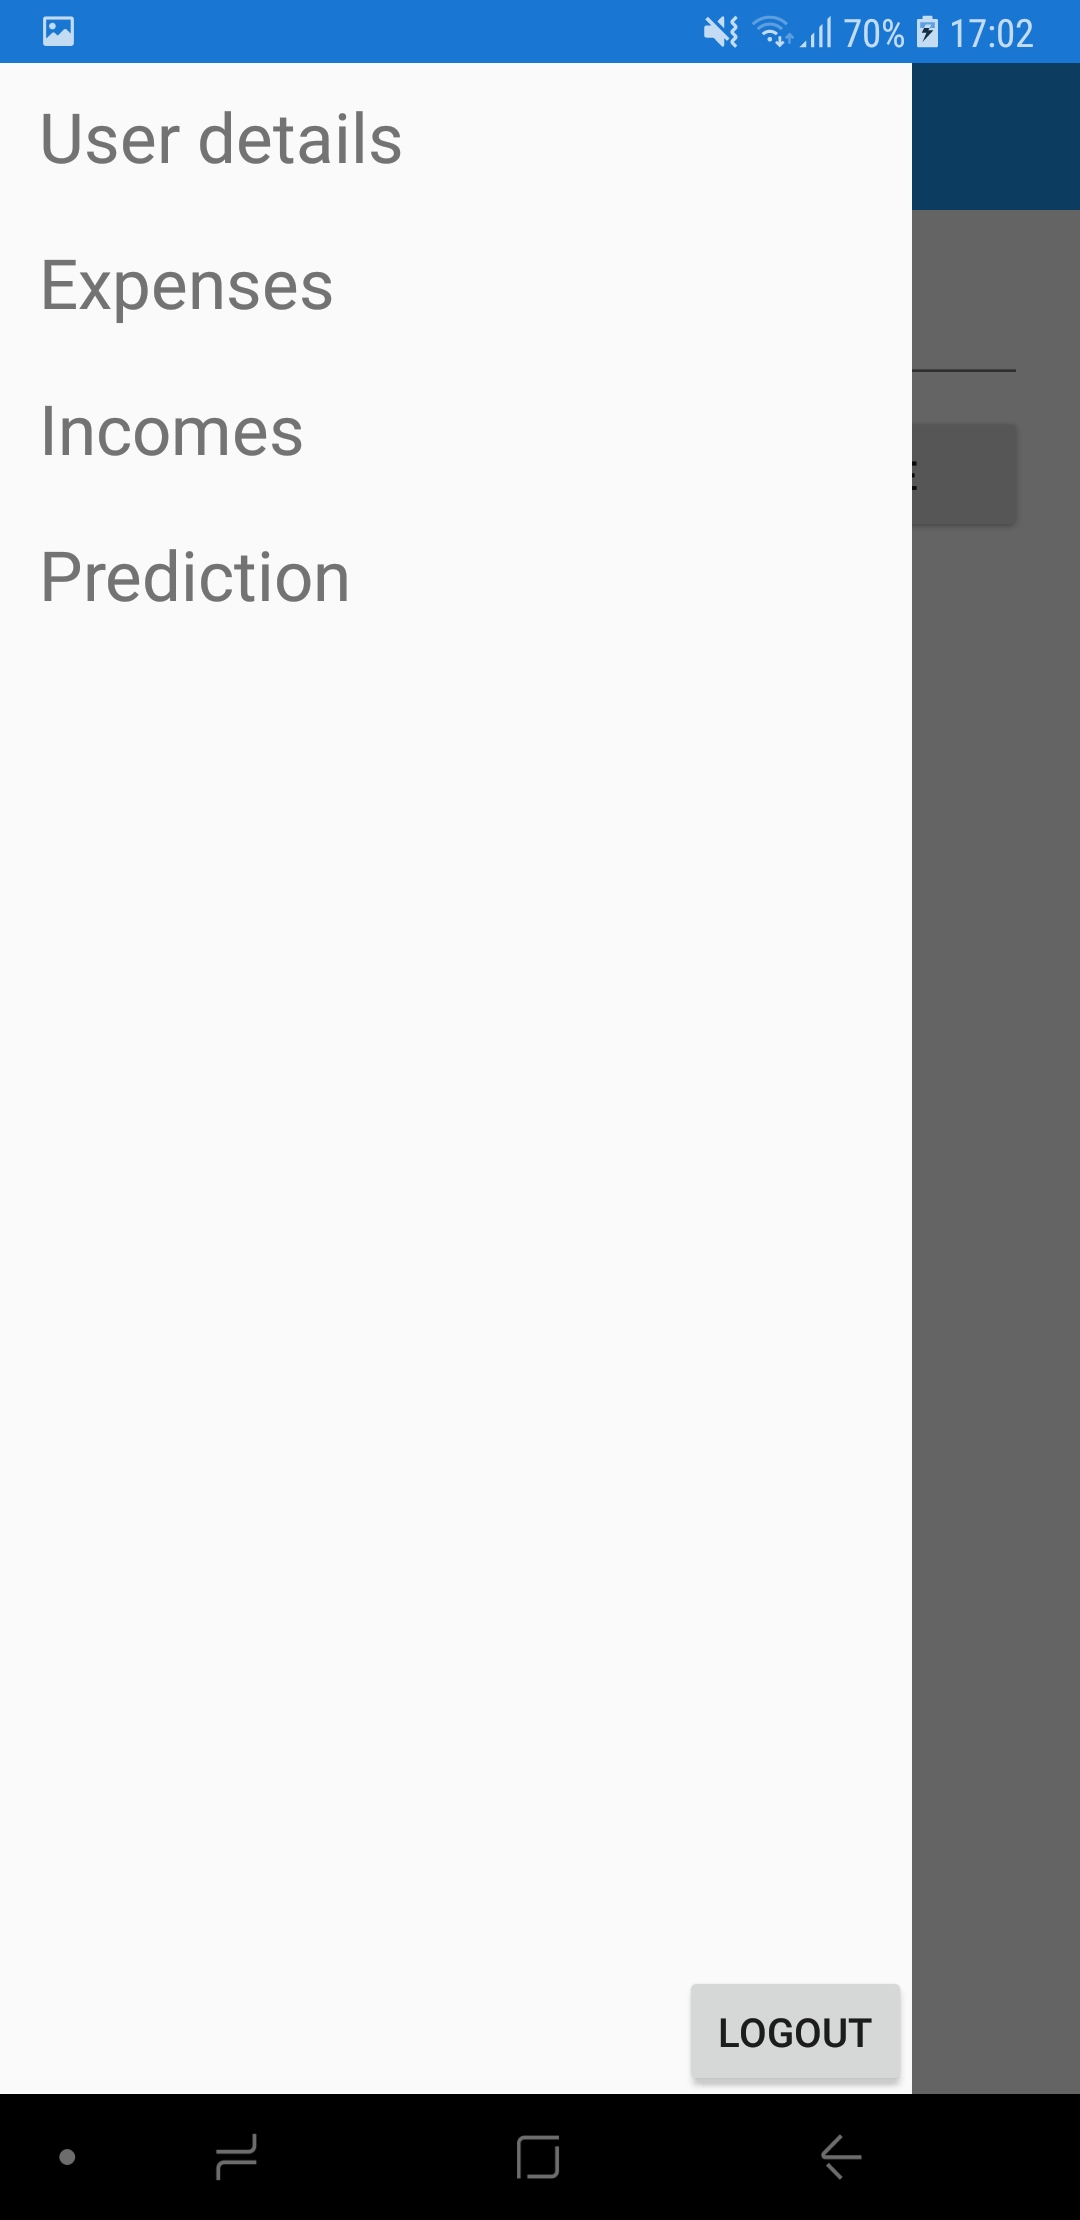
\includegraphics[width=1.75in]{img/mobile/menu_boczne.jpg}
			\subcaption{Menu boczne.}
			\label{hamburger_przychody}
		\end{subfigure}
		\begin{subfigure}[b]{0.3\textwidth}
			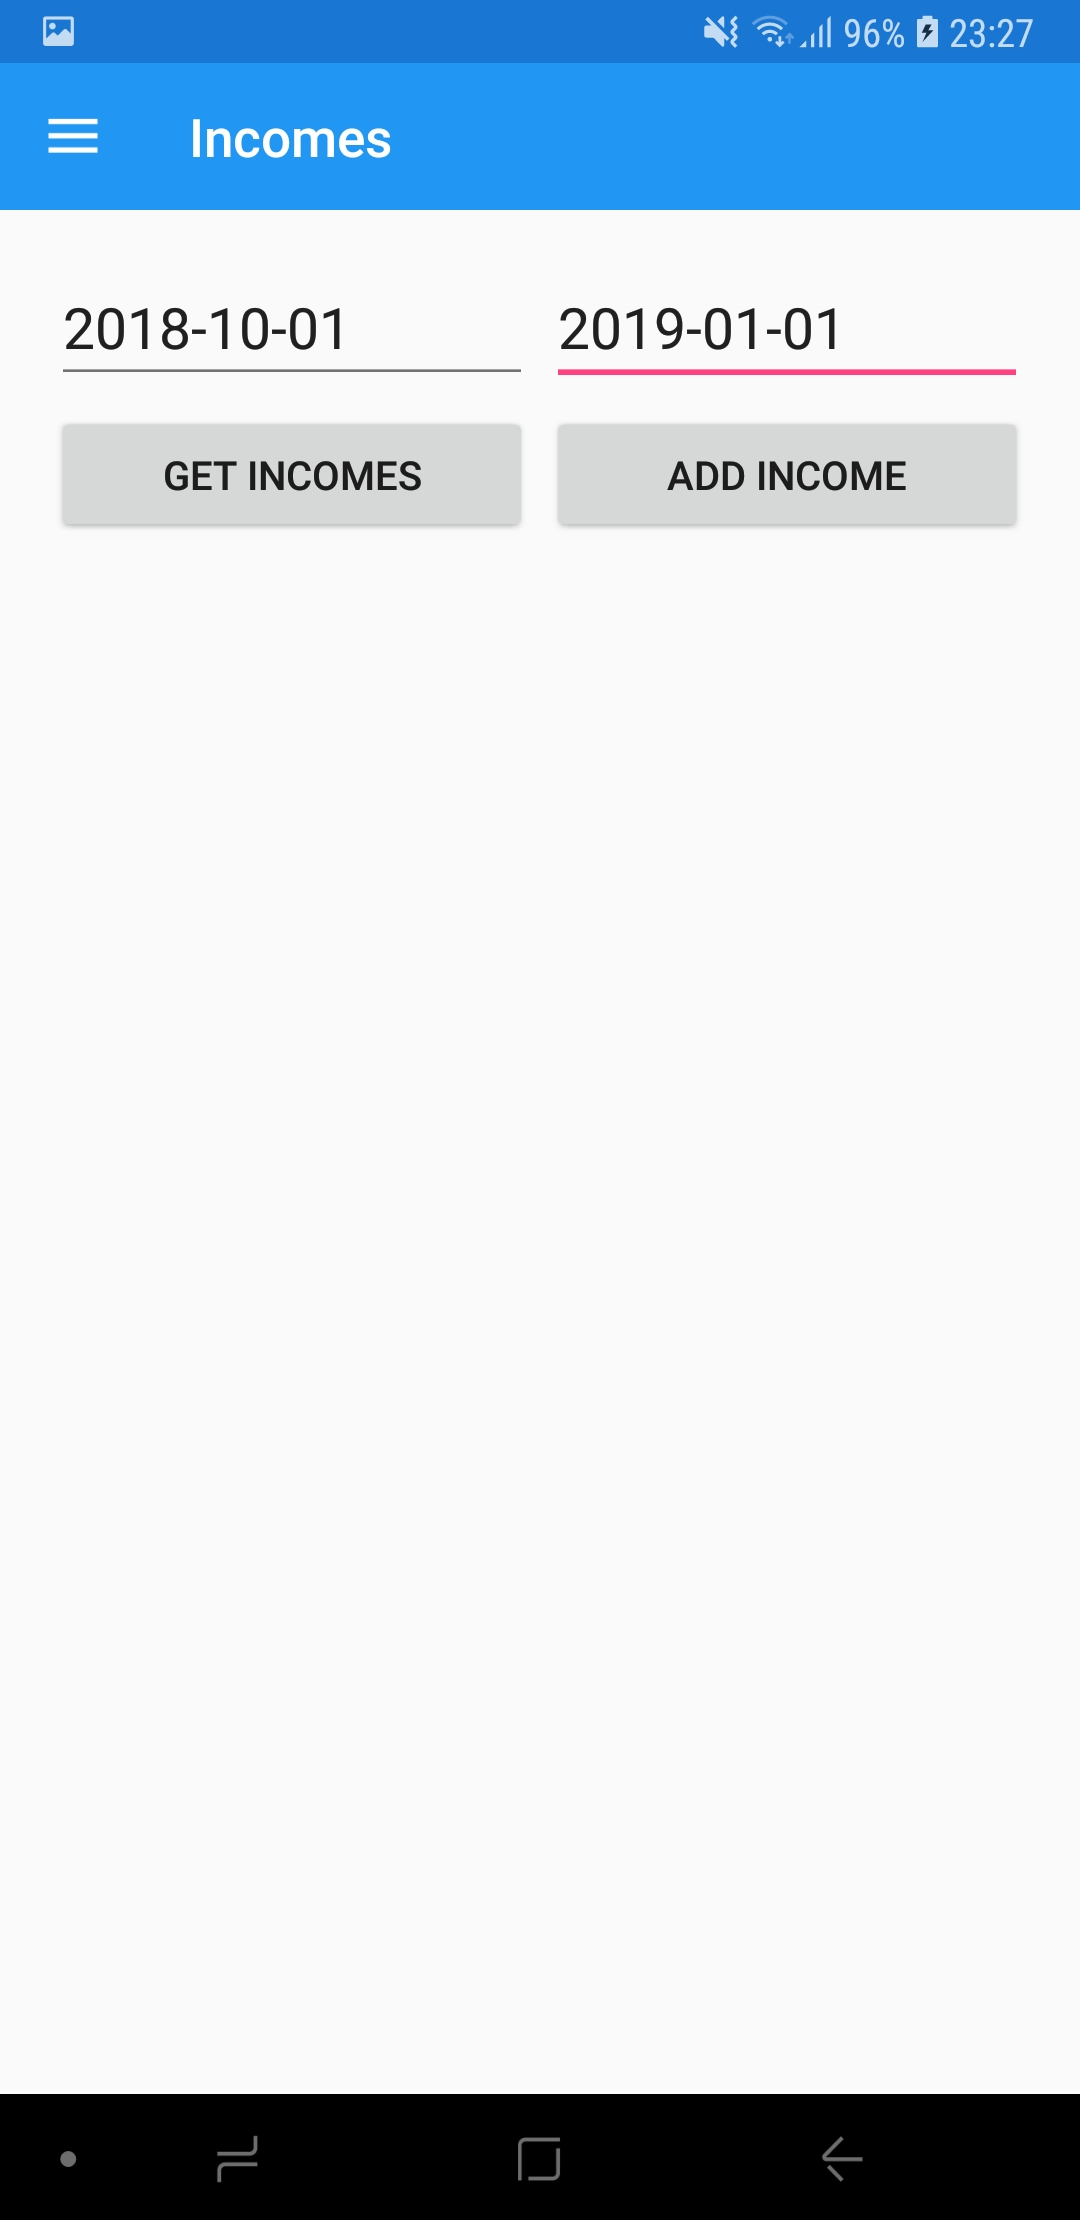
\includegraphics[width=1.75in]{img/mobile/przychody.jpg}
			\subcaption{Strona z przychodami.}
			\label{przychody}
		\end{subfigure}
		\begin{subfigure}[b]{0.3\textwidth}
			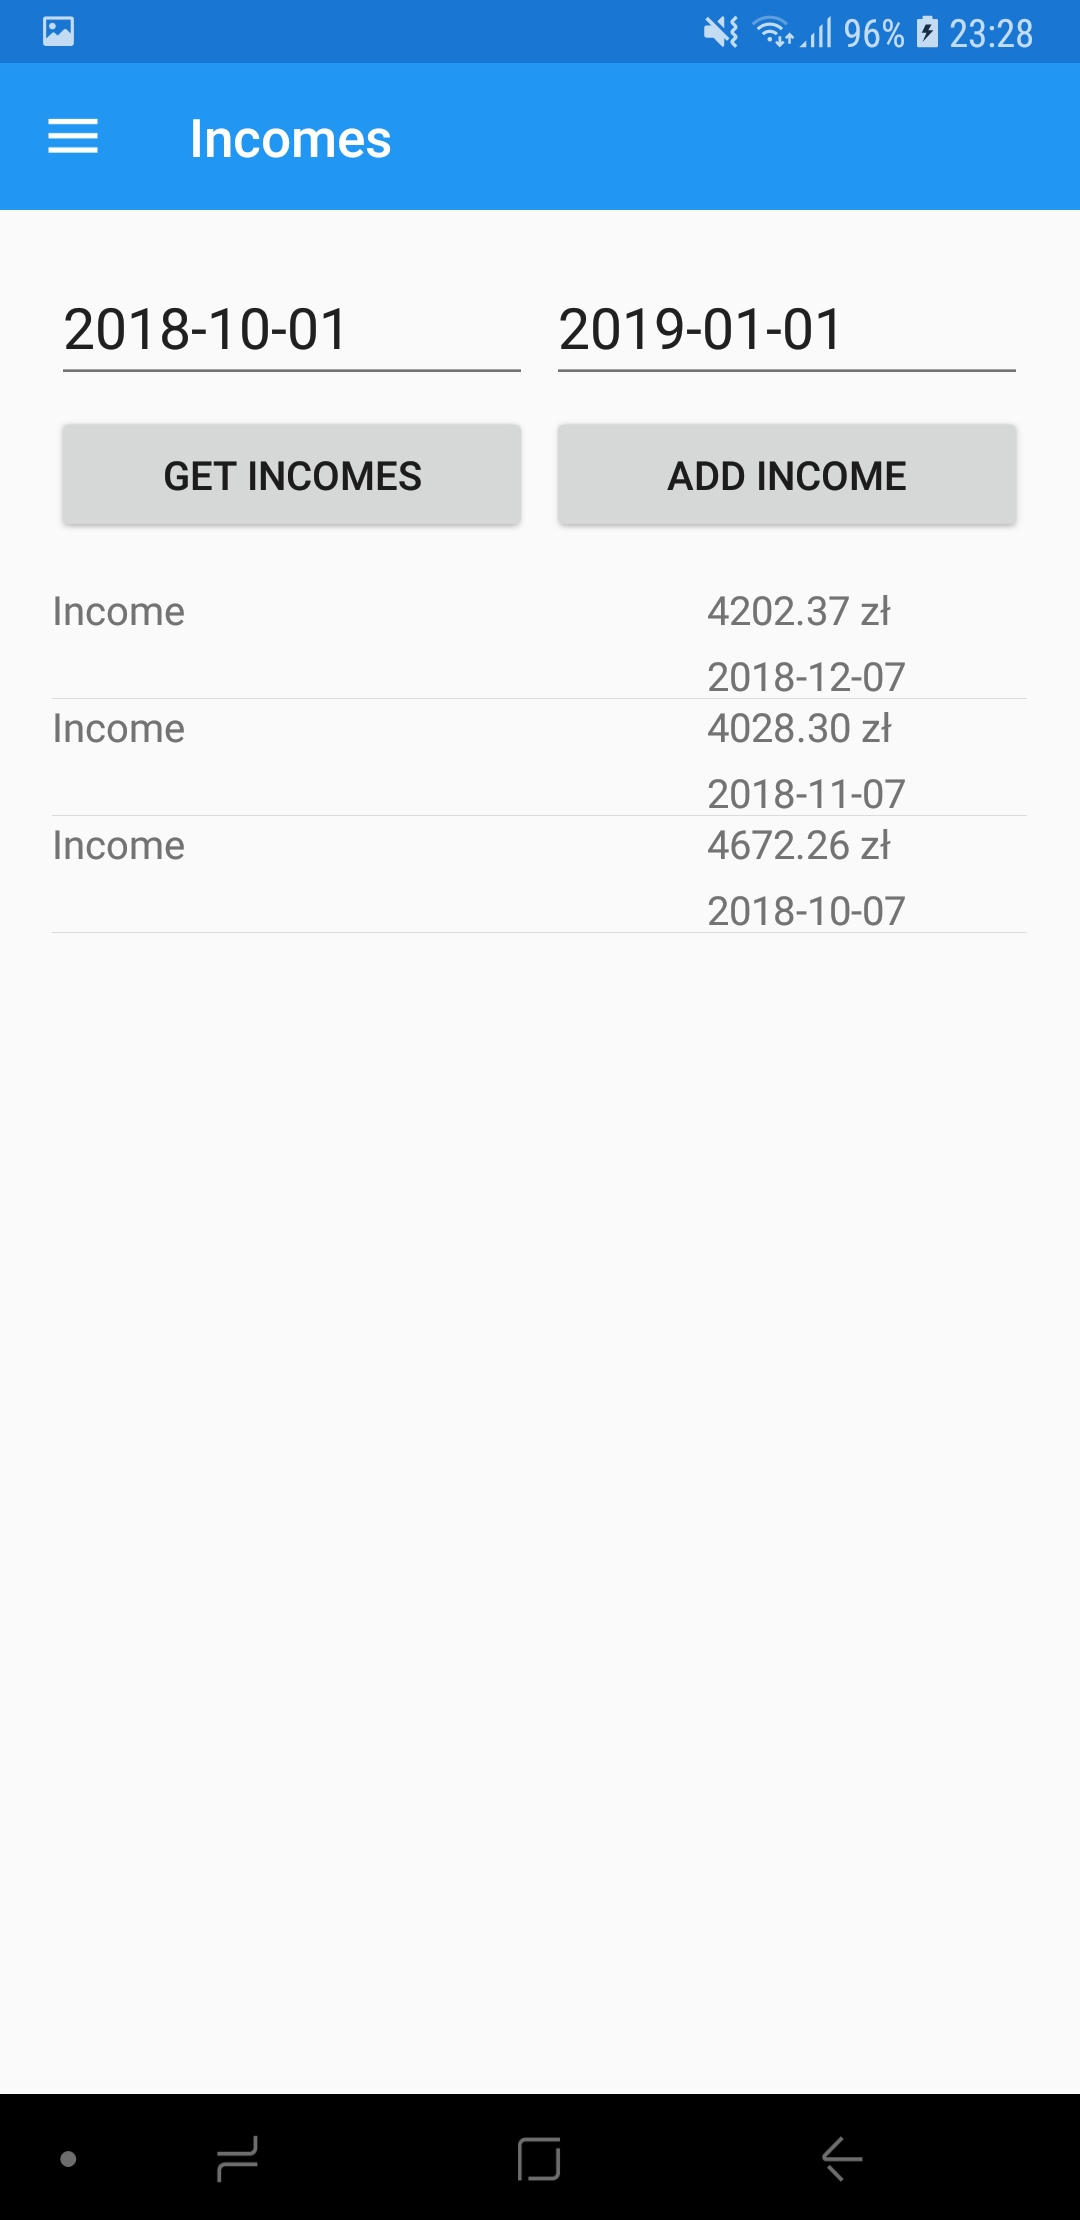
\includegraphics[width=1.75in]{img/mobile/przychody_gotowe.jpg}
			\subcaption{Lista przychodów.}
			\label{przychody_gotowe}
		\end{subfigure}
	\end{center}
	\caption{Zrzuty ekranu procesu wyświetlania przychodów.}
\end{figure}

\textbf{Dodawanie przychodu} (przypadek użycia "dodaj przychód") - dodanie wpisu z przychodem uwierzytelnionego użytkownika. Wybranie przycisku "ADD INCOME" na stronie przychodów (Rys. \ref{(przychody_dodaj}) powoduje wyświetlenie formularza dodawania przychodu (Rys. \ref{dodaj_przychod}). Po wypełnieniu formularza przy pomocy przycisku "ADD" przychód jest dodawany, a przycisk "BACK" skutkuje powrotem do strony przychodów.
\begin{figure}[!ht]
	\begin{center}
		\begin{subfigure}[b]{0.3\textwidth}
			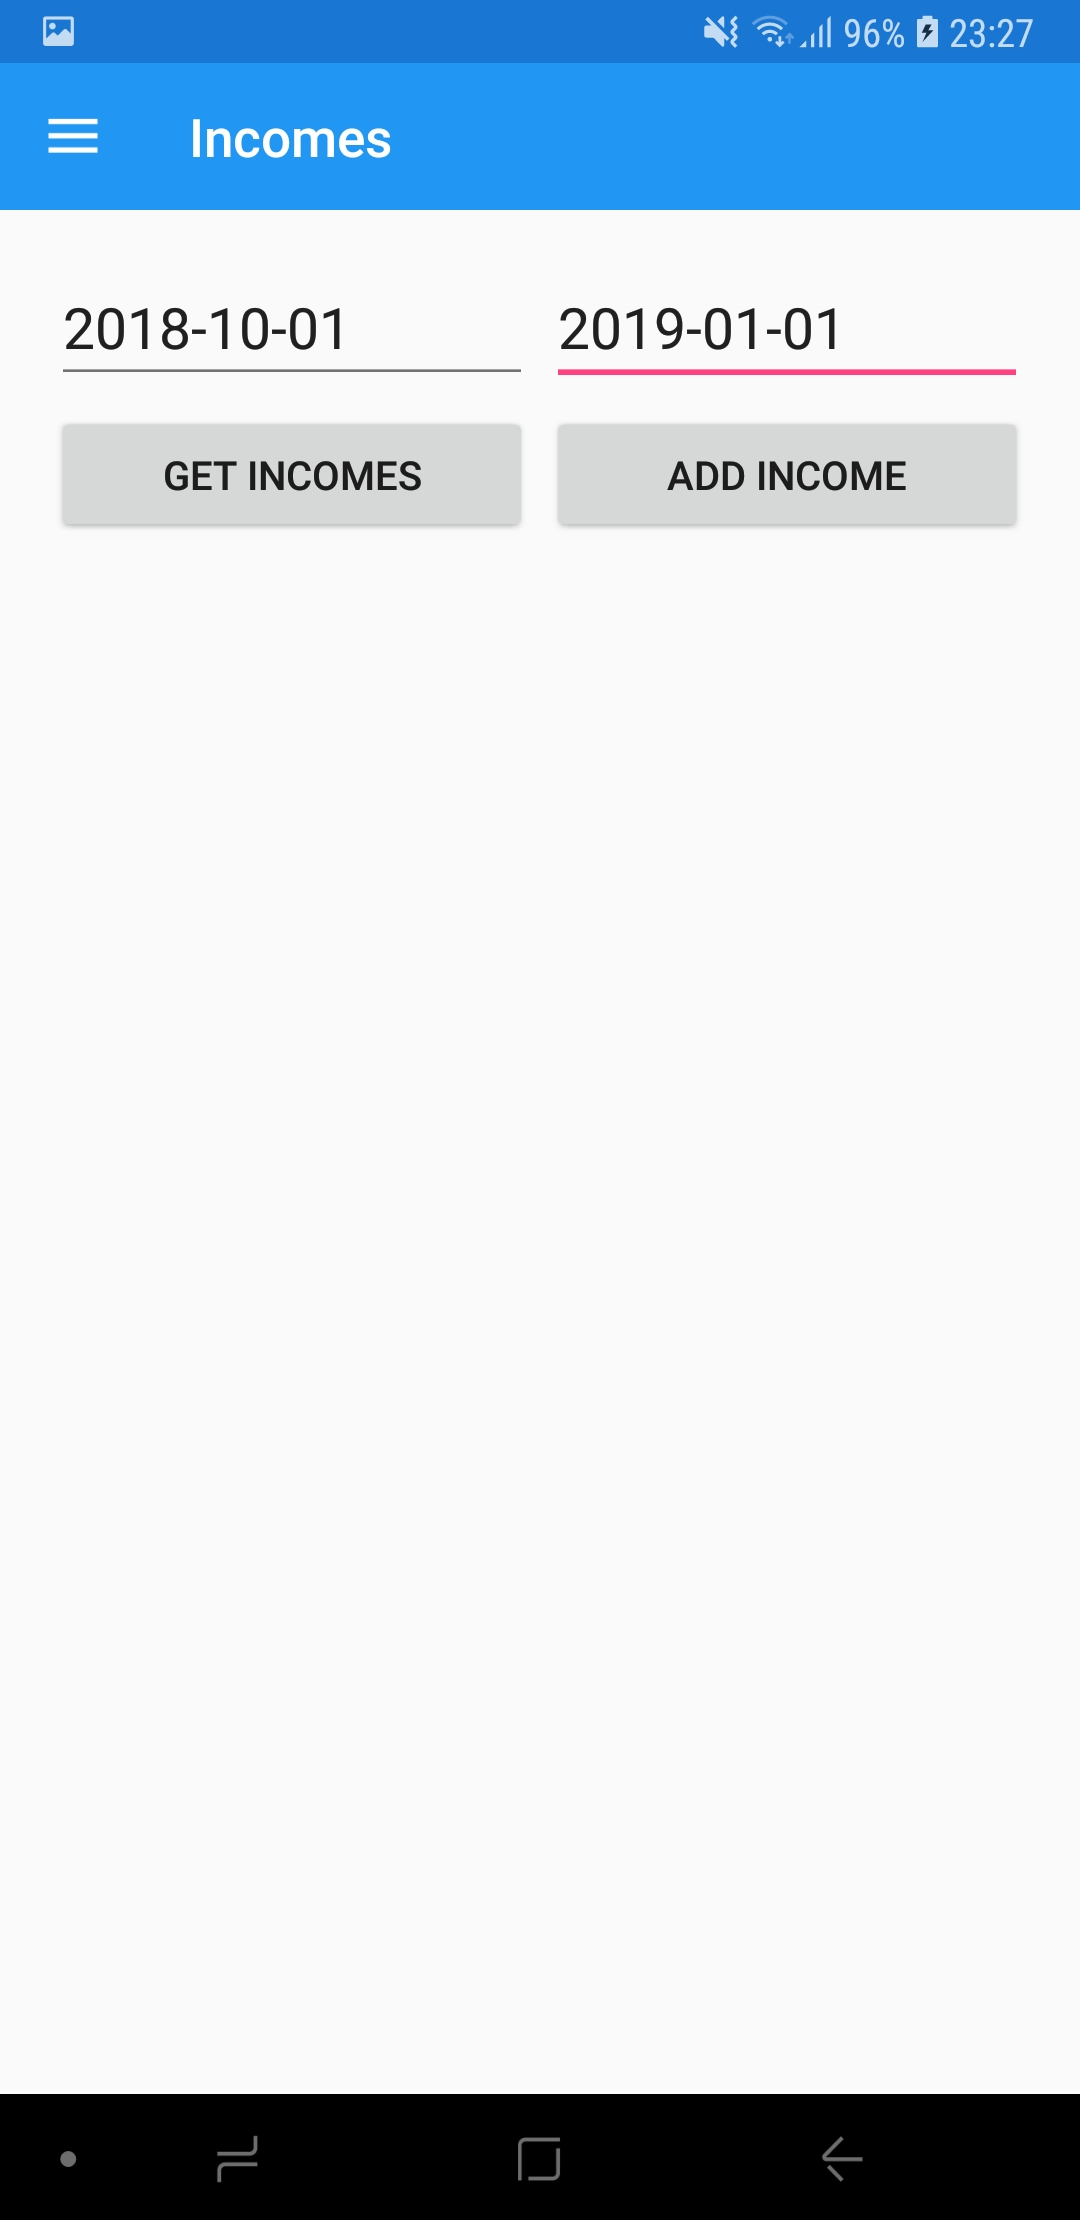
\includegraphics[width=1.75in]{img/mobile/przychody.jpg}
			\subcaption{Strona przychodów.\newline}
			\label{przychody_dodaj}
		\end{subfigure}
		\begin{subfigure}[b]{0.3\textwidth}
			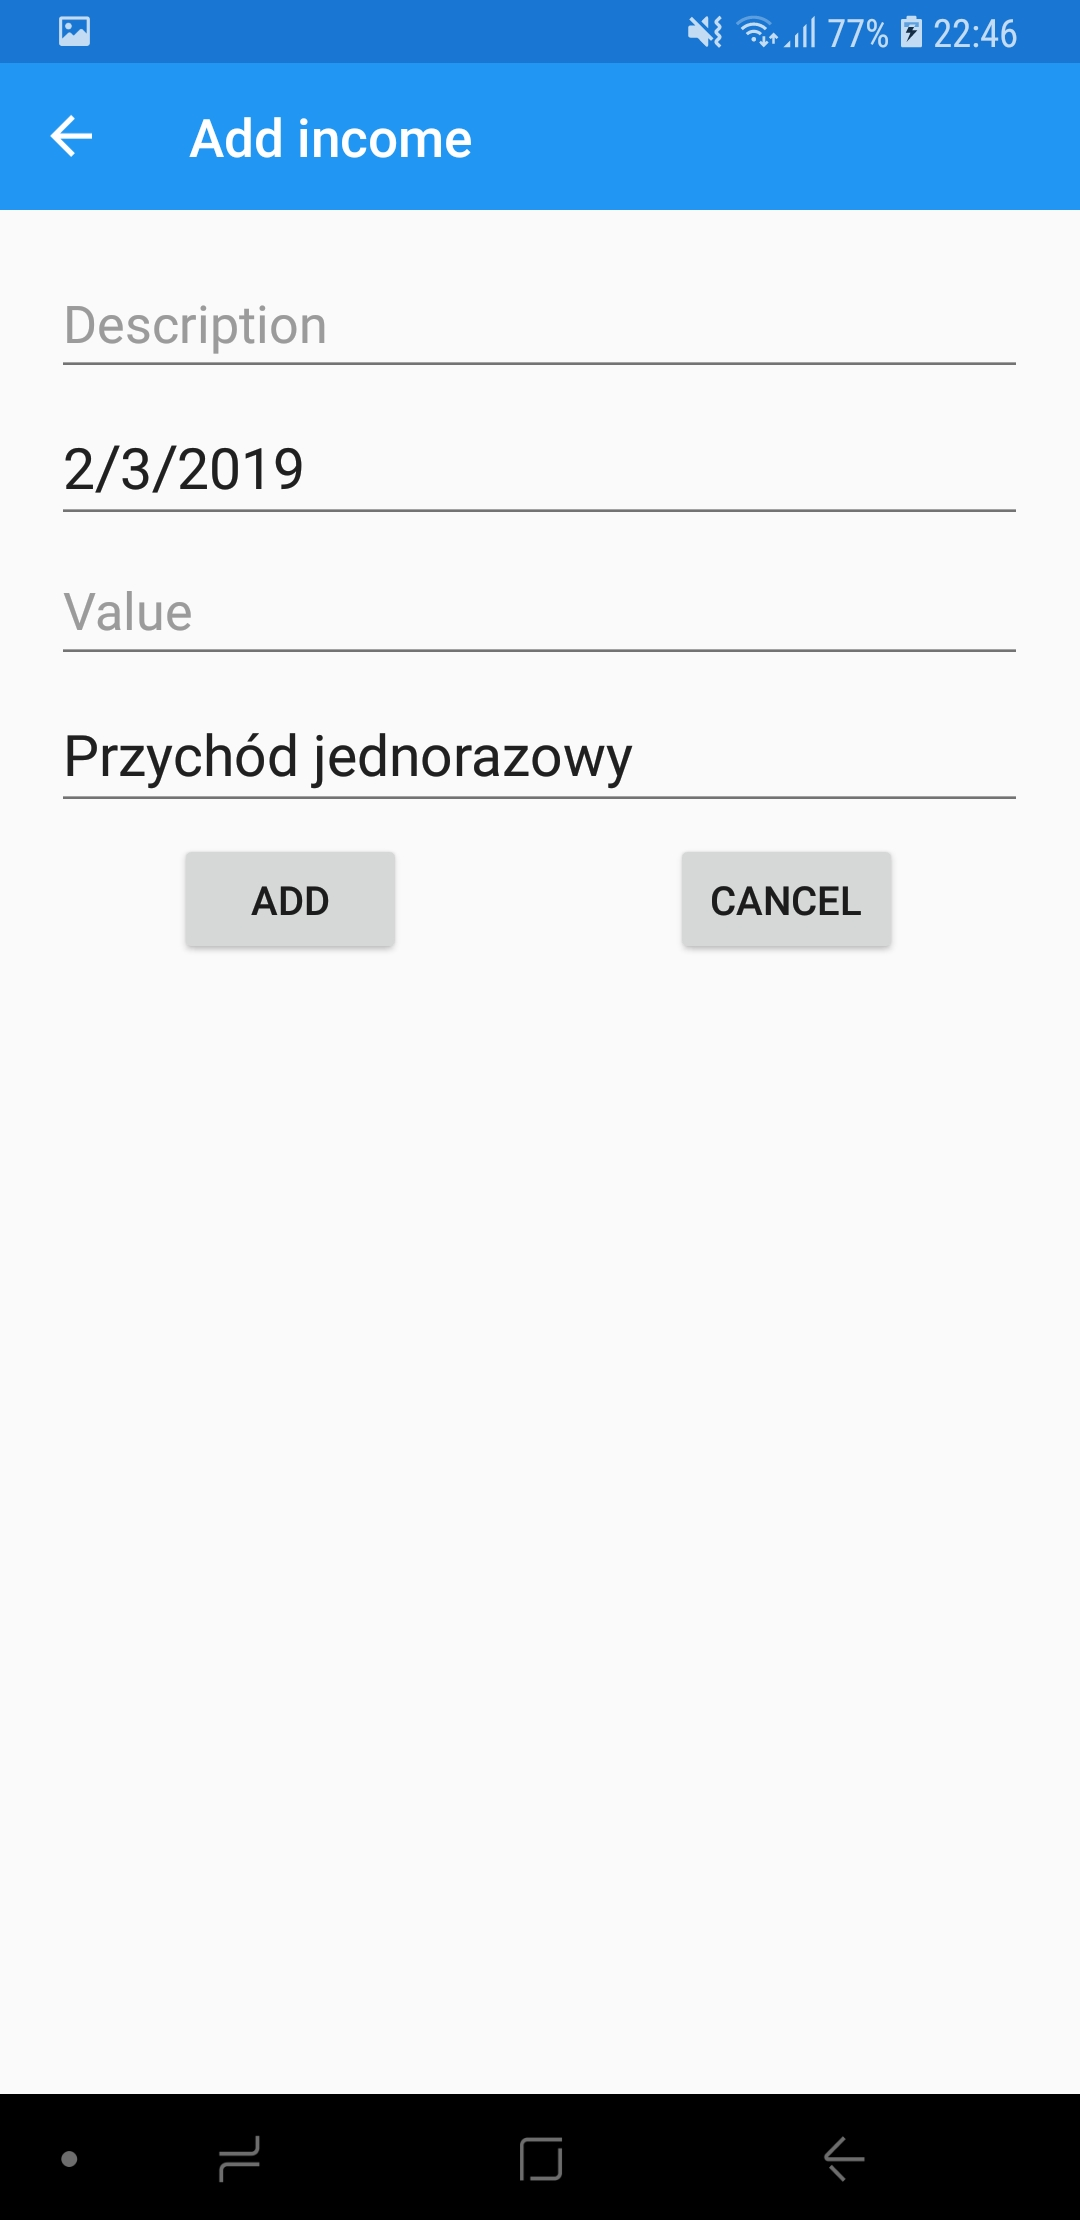
\includegraphics[width=1.75in]{img/mobile/dodaj_przychod.jpg}
			\subcaption{Formularz dodawania przychodu.}
			\label{dodaj_przychod}
		\end{subfigure}
	\end{center}
	\caption{Zrzuty ekranu procesu dodawania przychodu.}
\end{figure}

\textbf{Edycja przychodu} (przypadek użycia "edytuj przychód") - zmiana wartości, opisu lub kategorii istniejącego przychodu uwierzytelnionego użytkownika. W widoku listy przychodów (Rys. \ref{przychody_lista}), naciśnięcie konkretnego przychodu powoduje wyświetlenie menu z opcjami (Rys. \ref{przychod_menu}). Po naciśnięciu "Edit" wyświetla się formularz z edycją przychodu (Rys. \ref{przychod_edycja}), który, po wypełnieniu, można wysłać przyciskiem "SUBMIT", co powoduje zapisanie zmian, lub powrócić do listy przychodów przyciskiem "BACK".
\begin{figure}[!ht]
	\begin{center}
		\begin{subfigure}[b]{0.3\textwidth}
			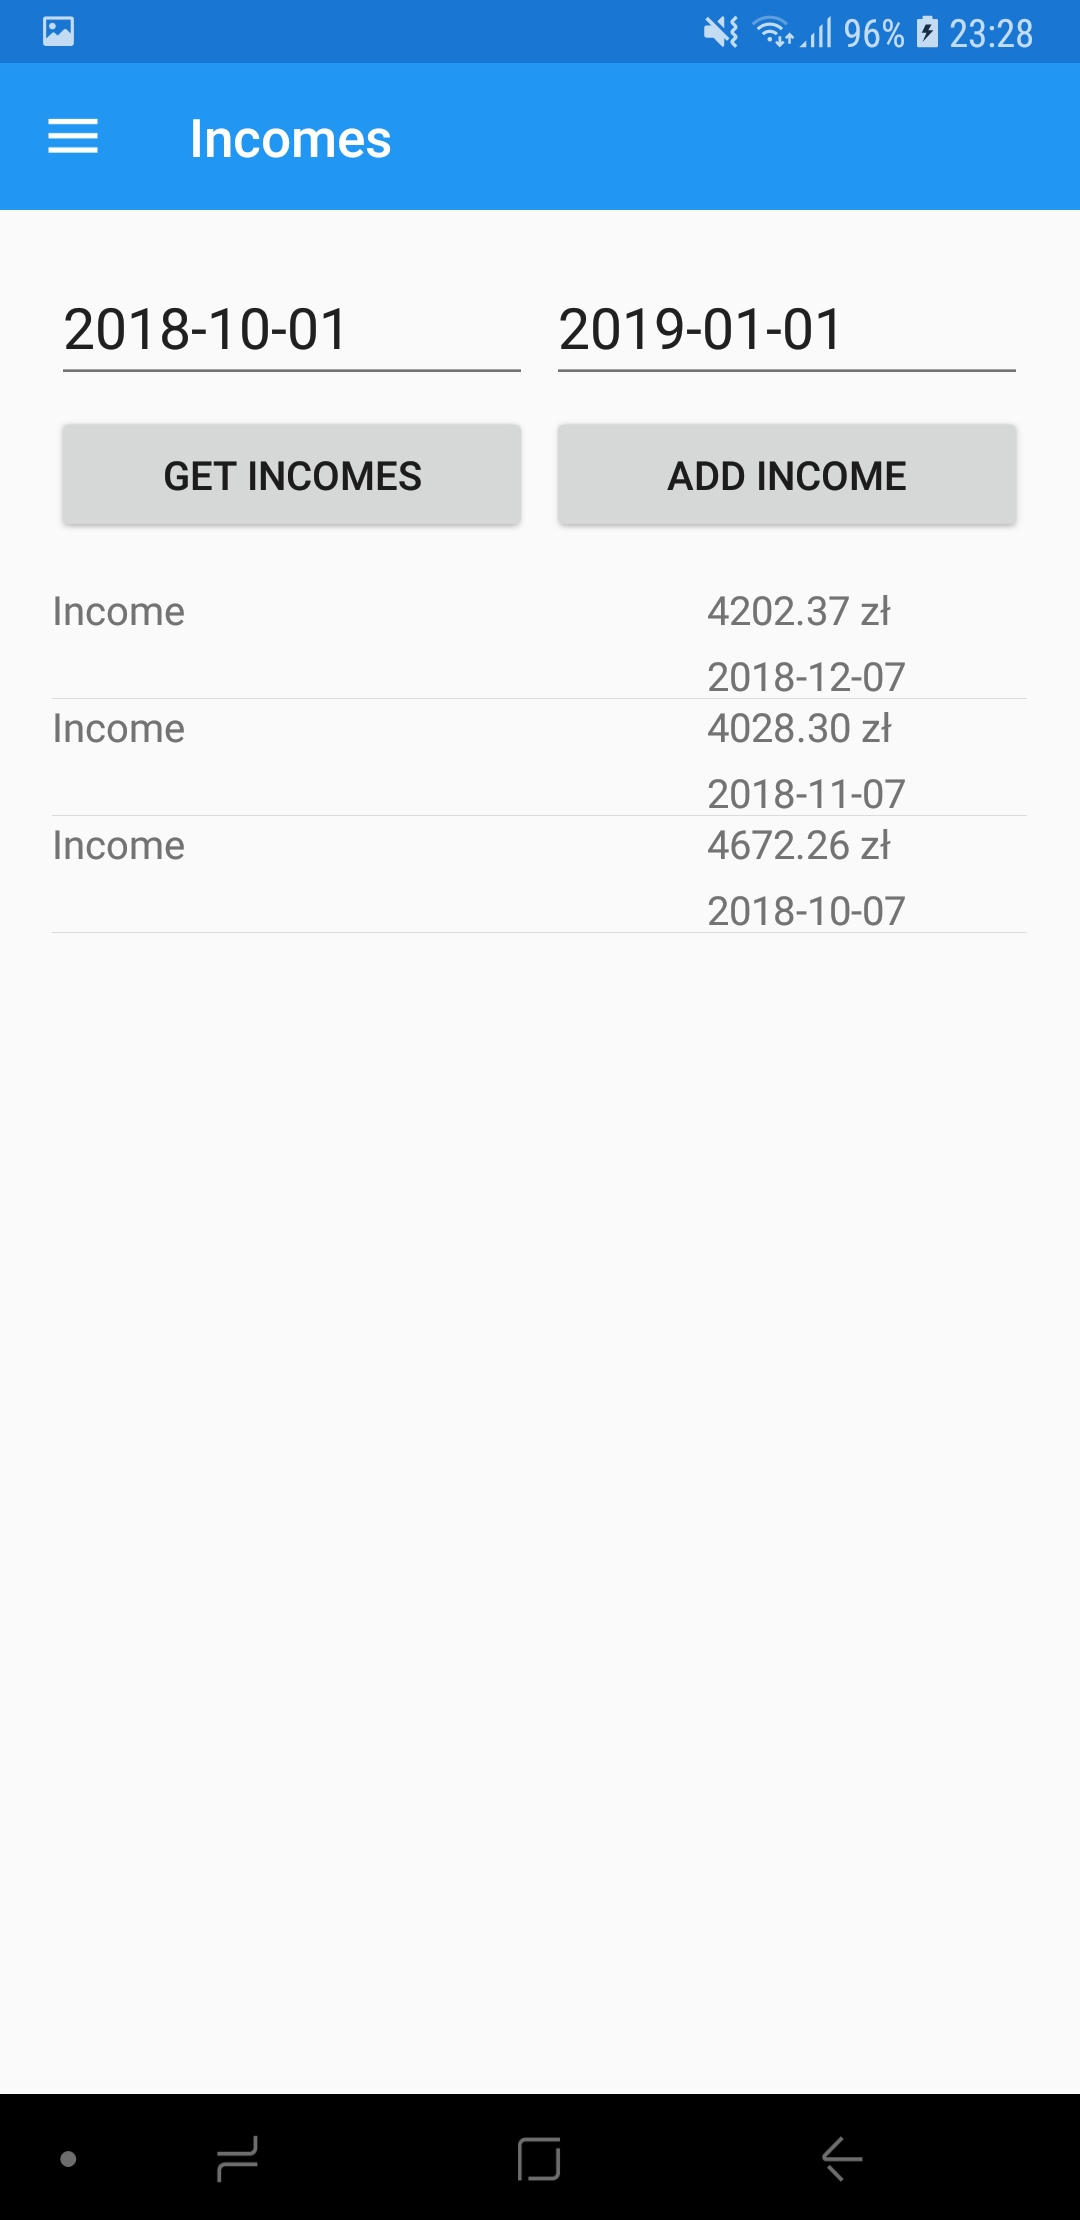
\includegraphics[width=1.75in]{img/mobile/przychody_gotowe.jpg}
			\subcaption{Lista przychodów.\newline}
			\label{przychody_lista}
		\end{subfigure}
		\begin{subfigure}[b]{0.3\textwidth}
			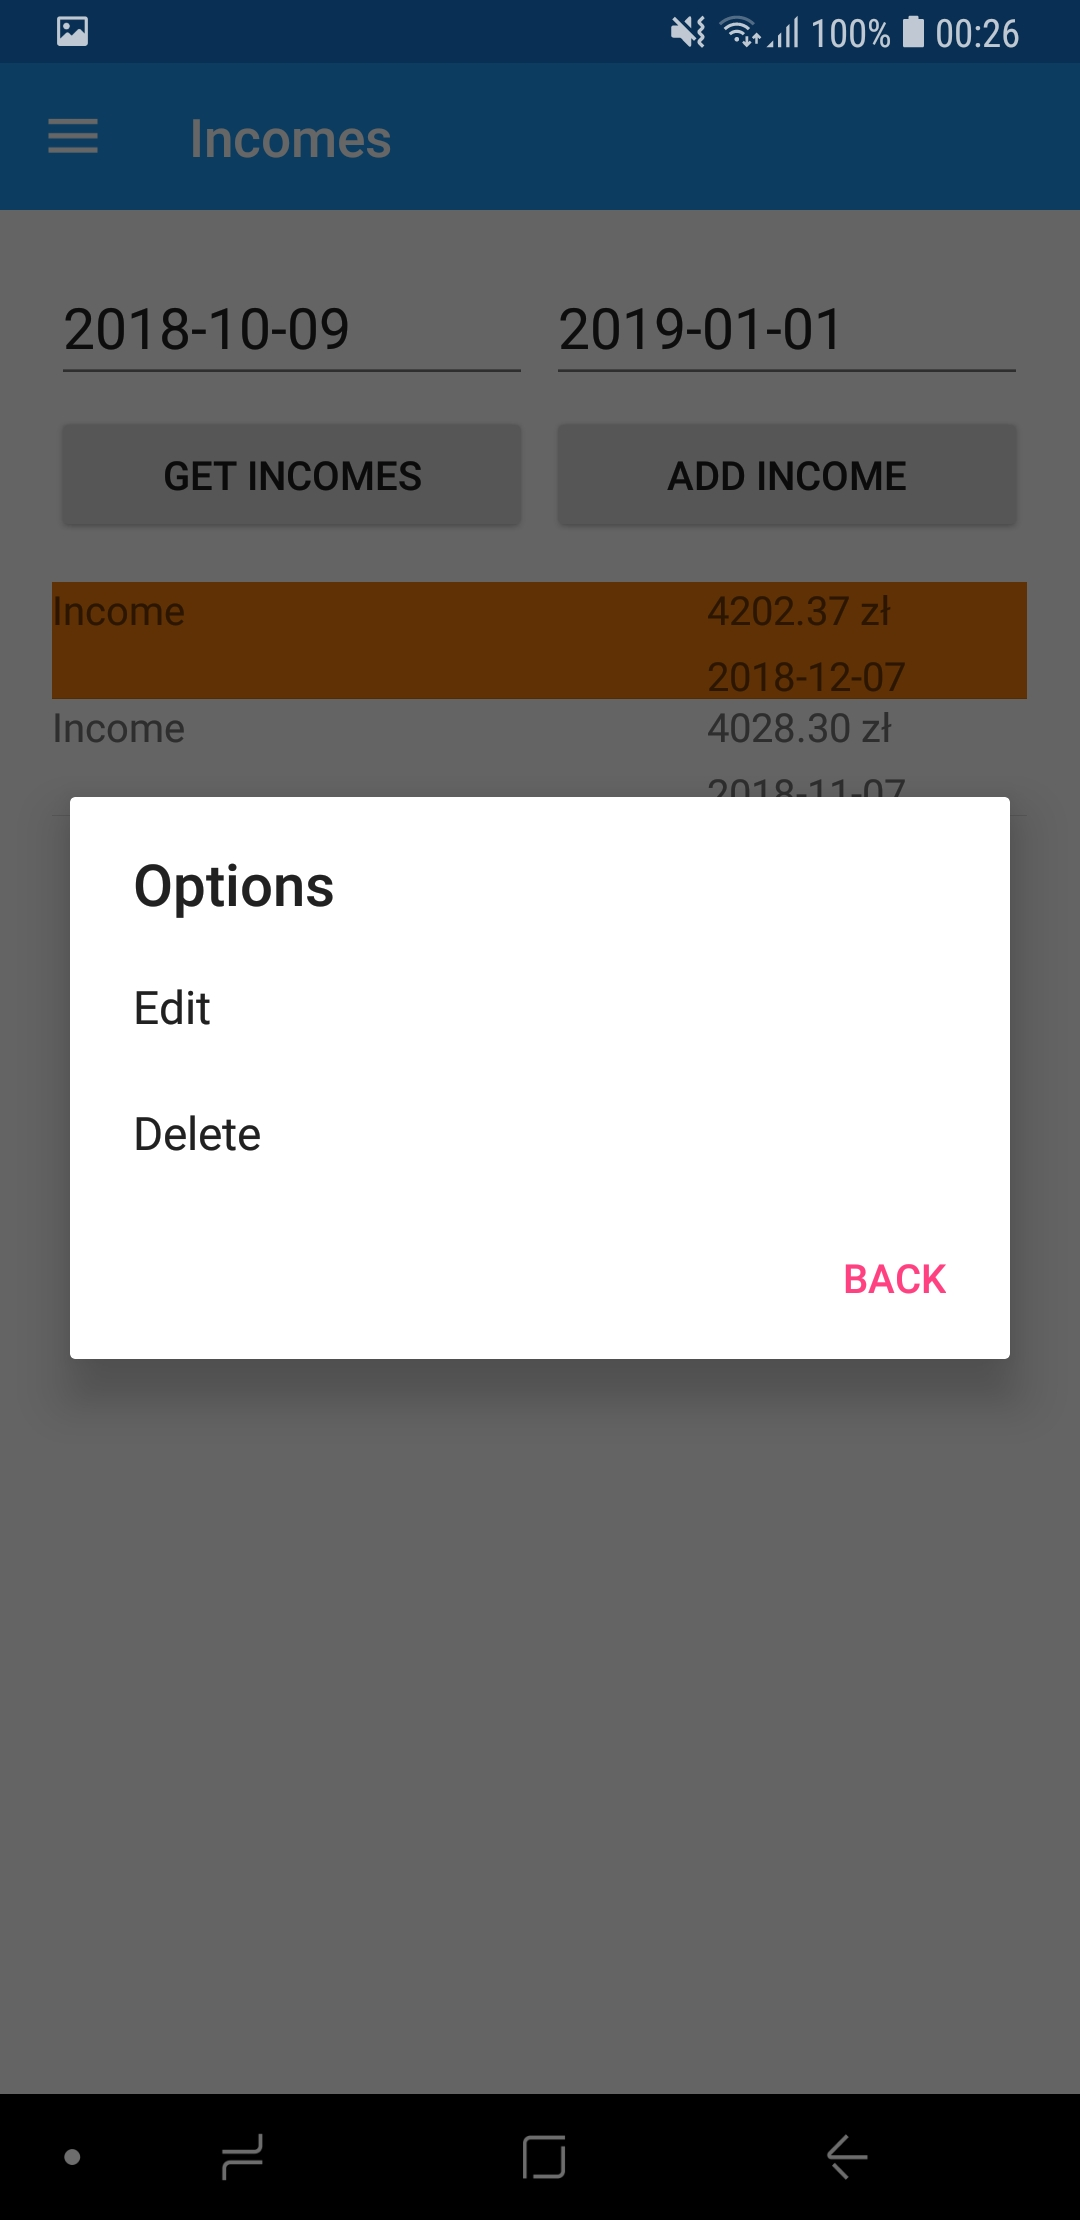
\includegraphics[width=1.75in]{img/mobile/przychod_menu.jpg}
			\subcaption{Menu przychodu.\newline}
			\label{przychod_menu}
		\end{subfigure}
		\begin{subfigure}[b]{0.3\textwidth}
			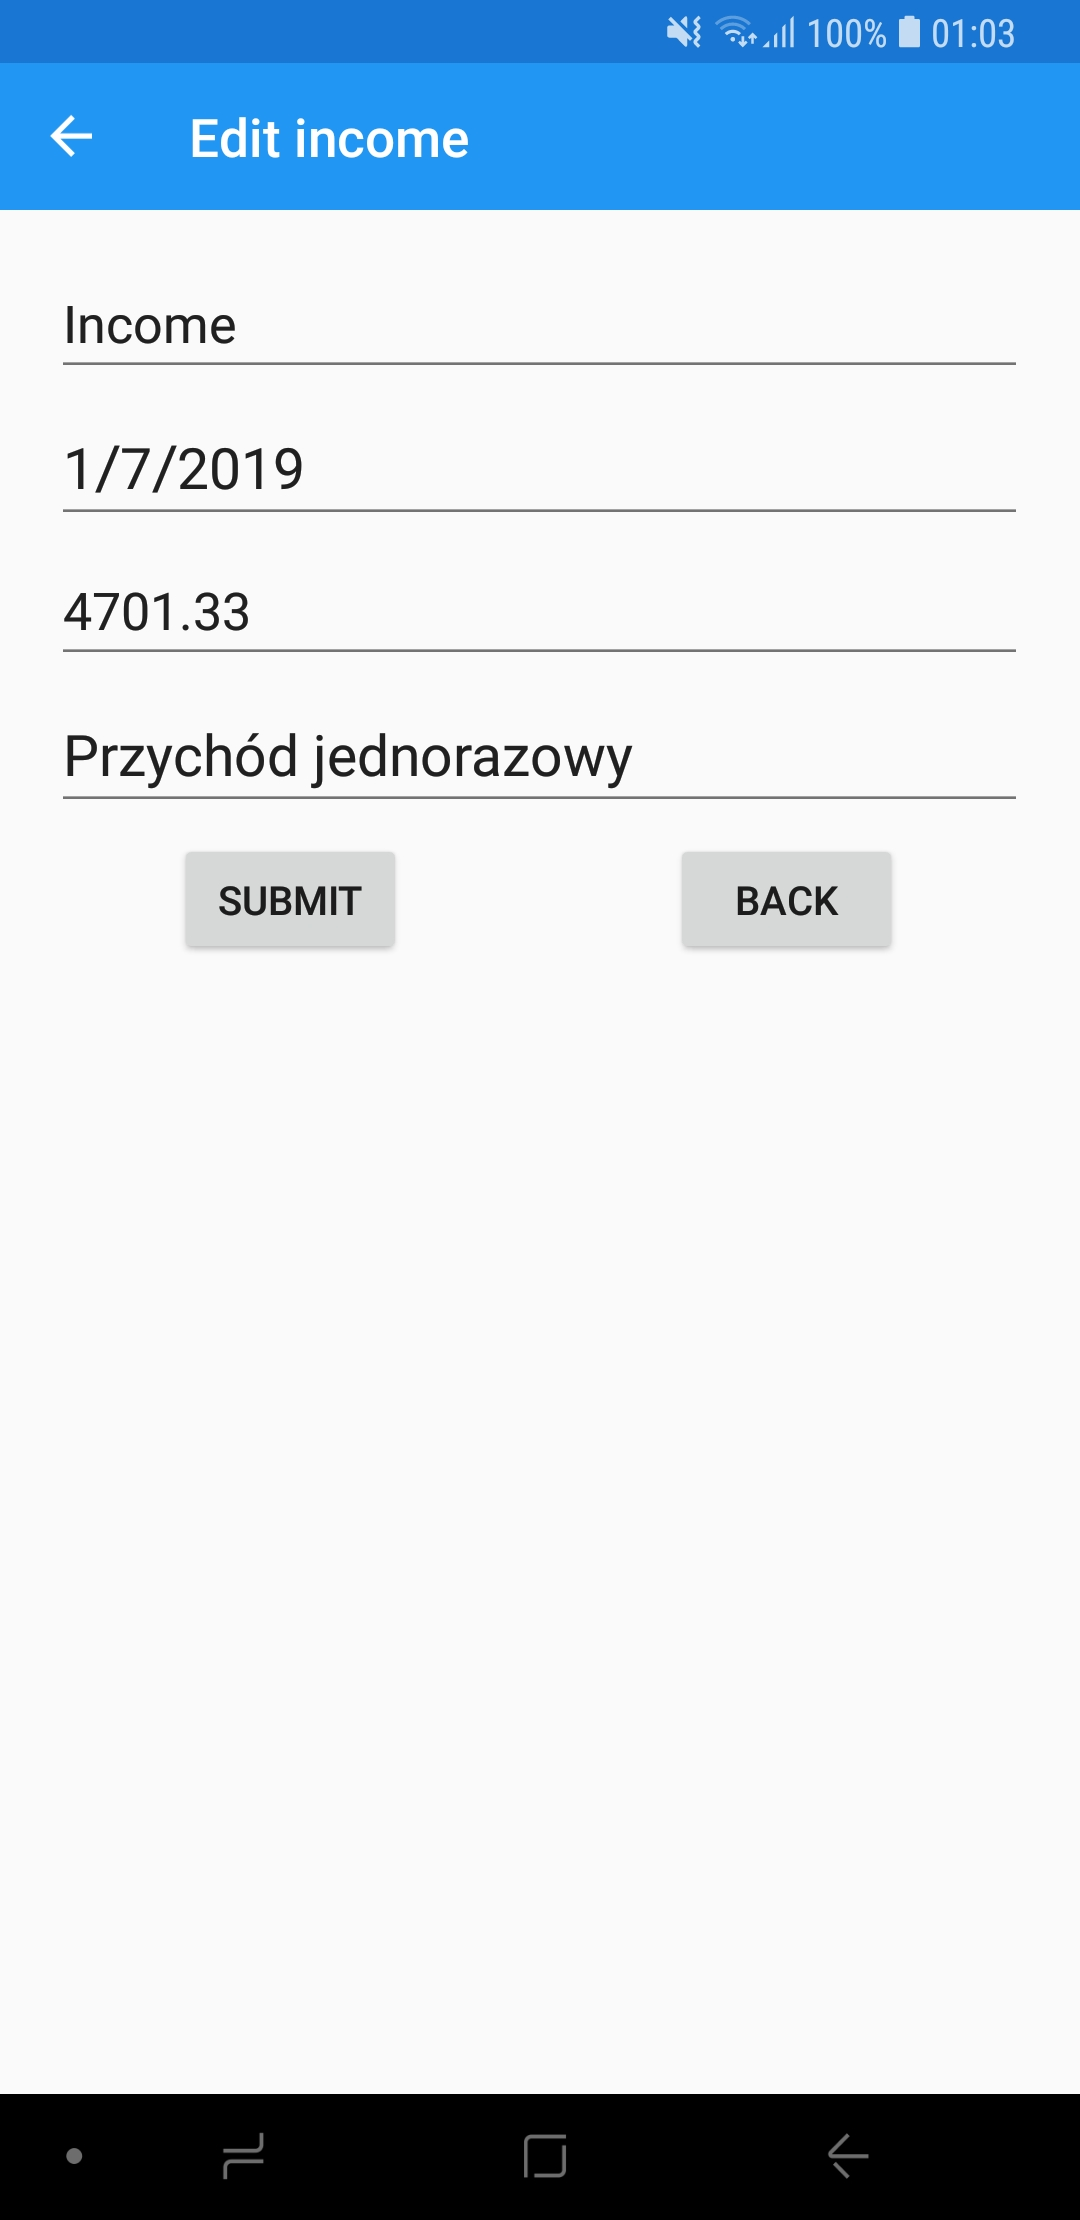
\includegraphics[width=1.75in]{img/mobile/przychod_edycja.jpg}
			\subcaption{Formularz edycji przychodu.}
			\label{przychod_edycja}
		\end{subfigure}
	\end{center}
	\caption{Zrzuty ekranu procesu edycji przychodu.}
\end{figure}

\textbf{Usuwanie przychodu} (przypadek użycia "usuń przychód") - usunięcie istniejącego przychodu należącego do aktualnie uwierzytelnionego użytkownika. Po naciśnięciu przychodu na liście przychodów (Rys. \ref{przychody_lista_usun}), wyświetlane jest menu (Rys. \ref{przychod_menu_usun}). Aby usunąć przychód należy w menu wybrać opcję "Delete" oraz potwierdzić chęć wykonania operacji (Rys. \ref{usun_na_pewno}).
\begin{figure}[!ht]
	\begin{center}
		\begin{subfigure}[b]{0.3\textwidth}
			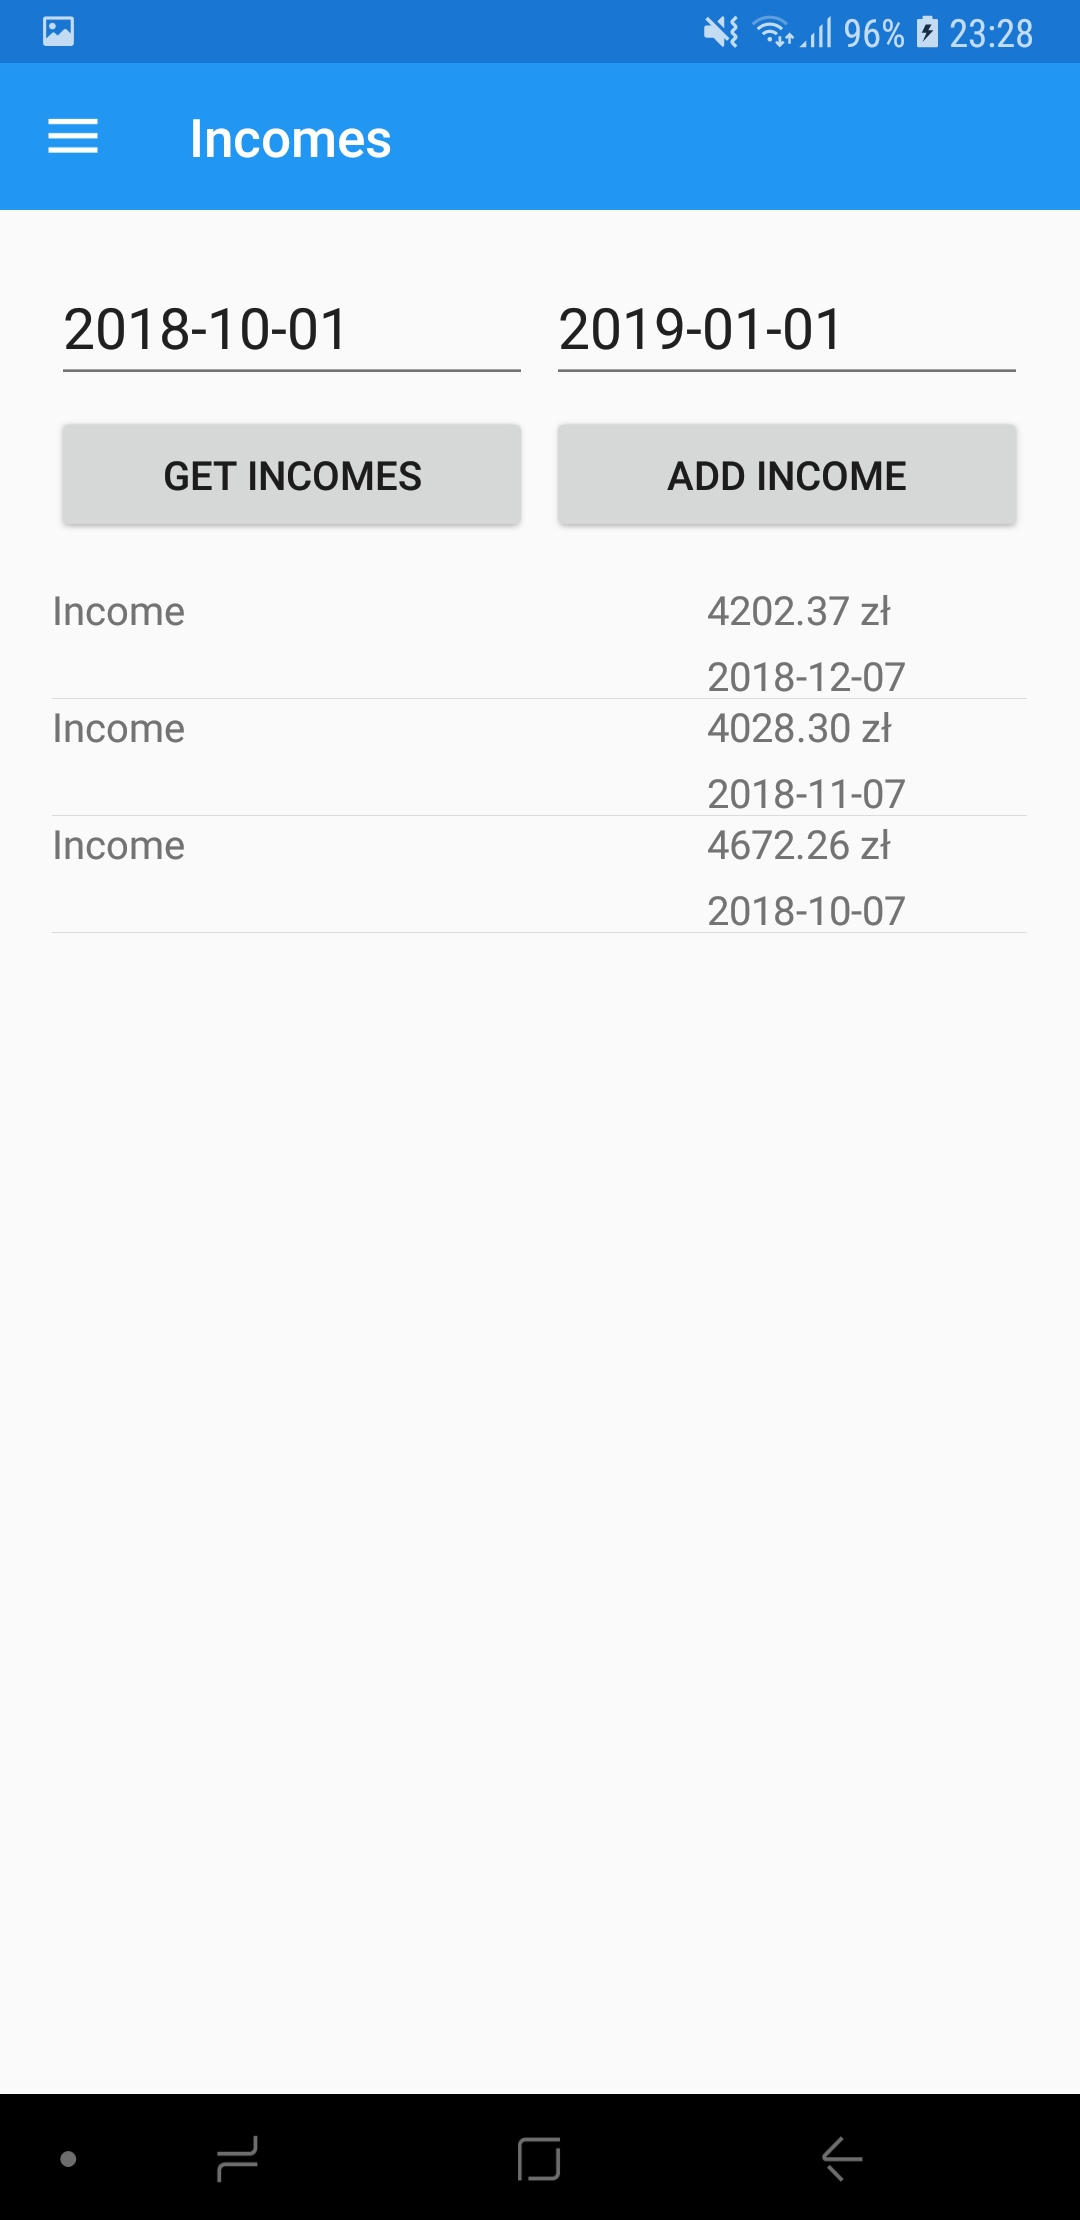
\includegraphics[width=1.75in]{img/mobile/przychody_gotowe.jpg}
			\subcaption{Lista przychodów.\newline}
			\label{przychody_lista_usun}
		\end{subfigure}
		\begin{subfigure}[b]{0.3\textwidth}
			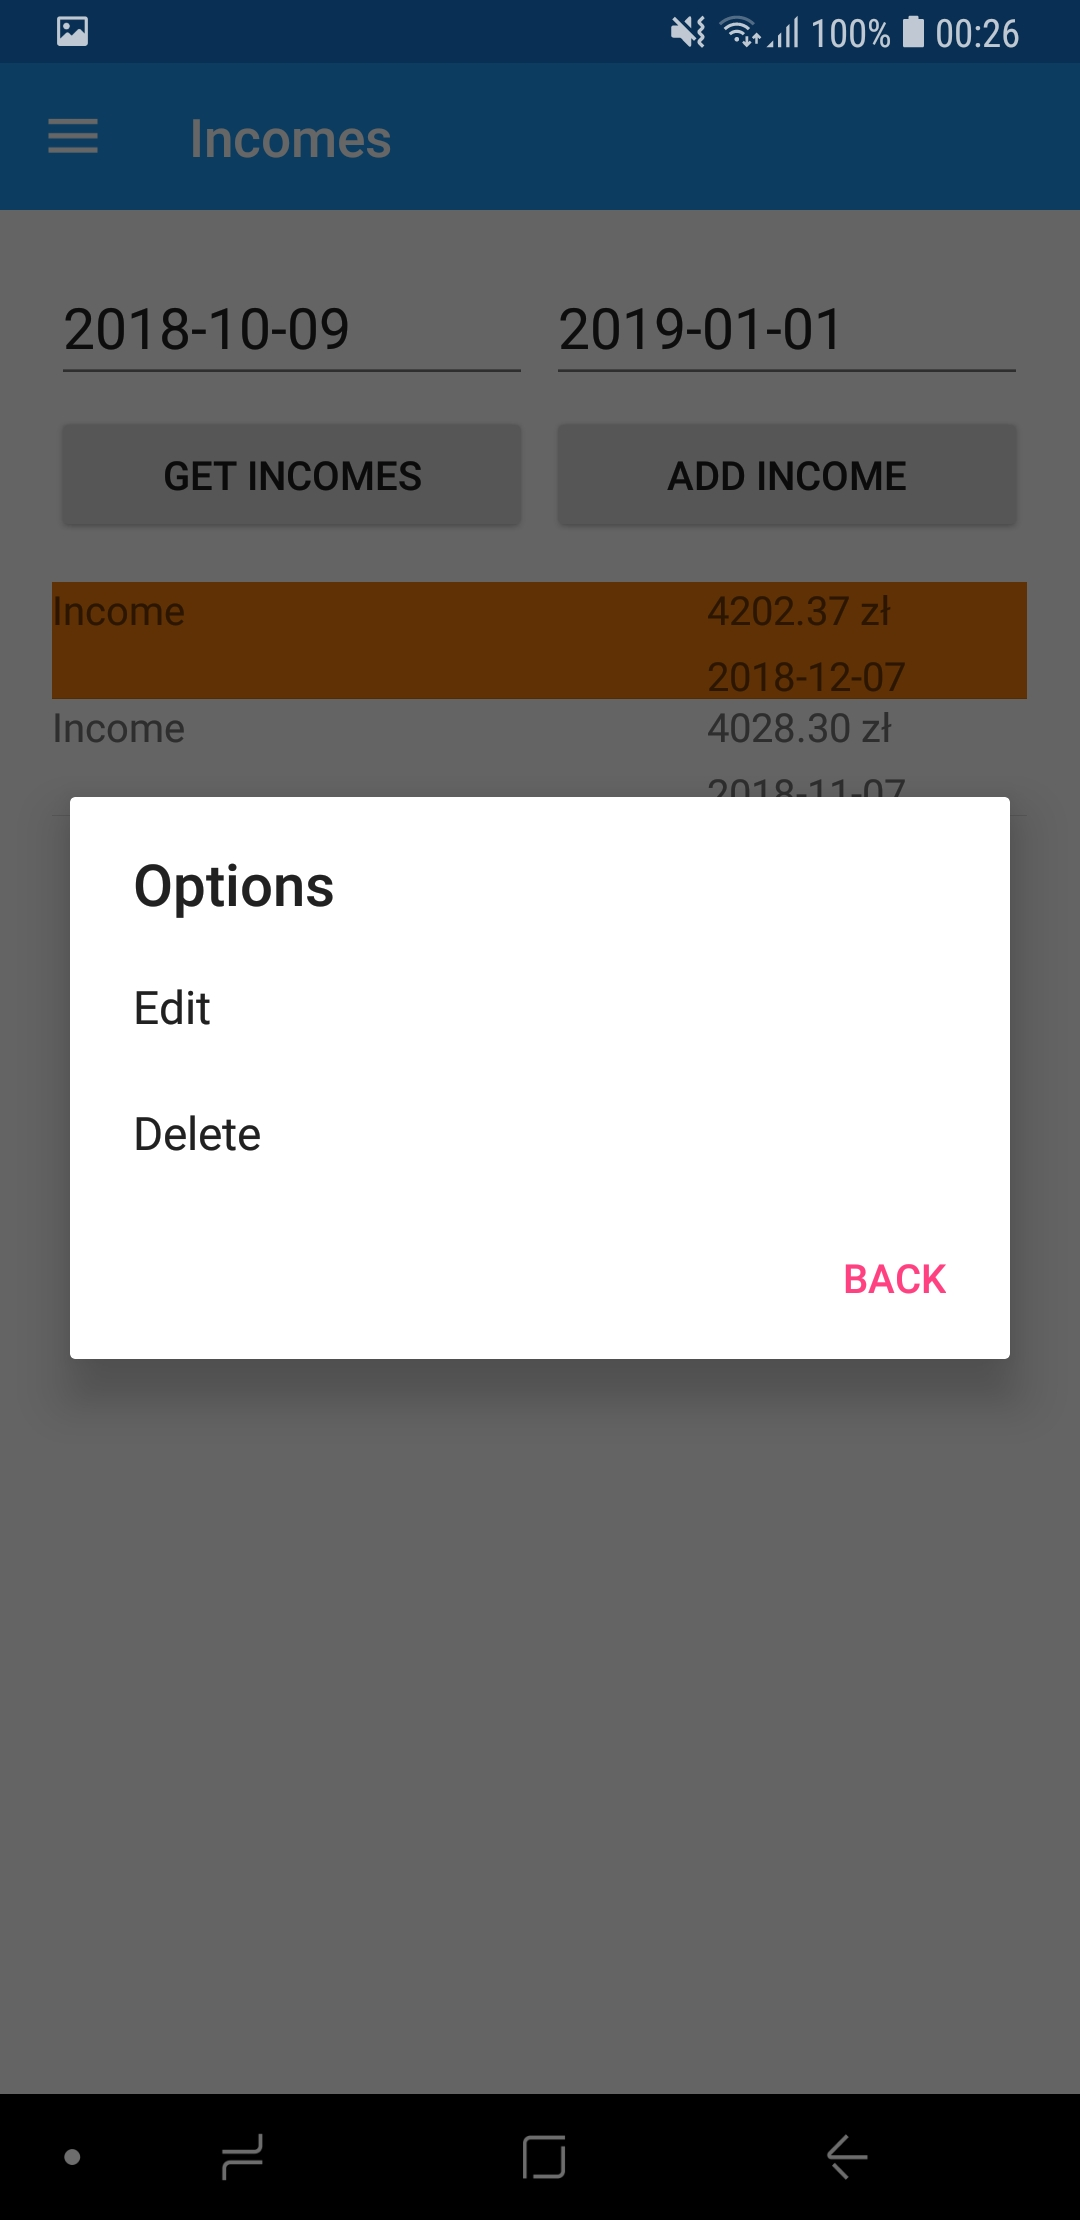
\includegraphics[width=1.75in]{img/mobile/przychod_menu.jpg}
			\subcaption{Menu przychodu.\newline}
			\label{przychod_menu_usun}
		\end{subfigure}
		\begin{subfigure}[b]{0.3\textwidth}
			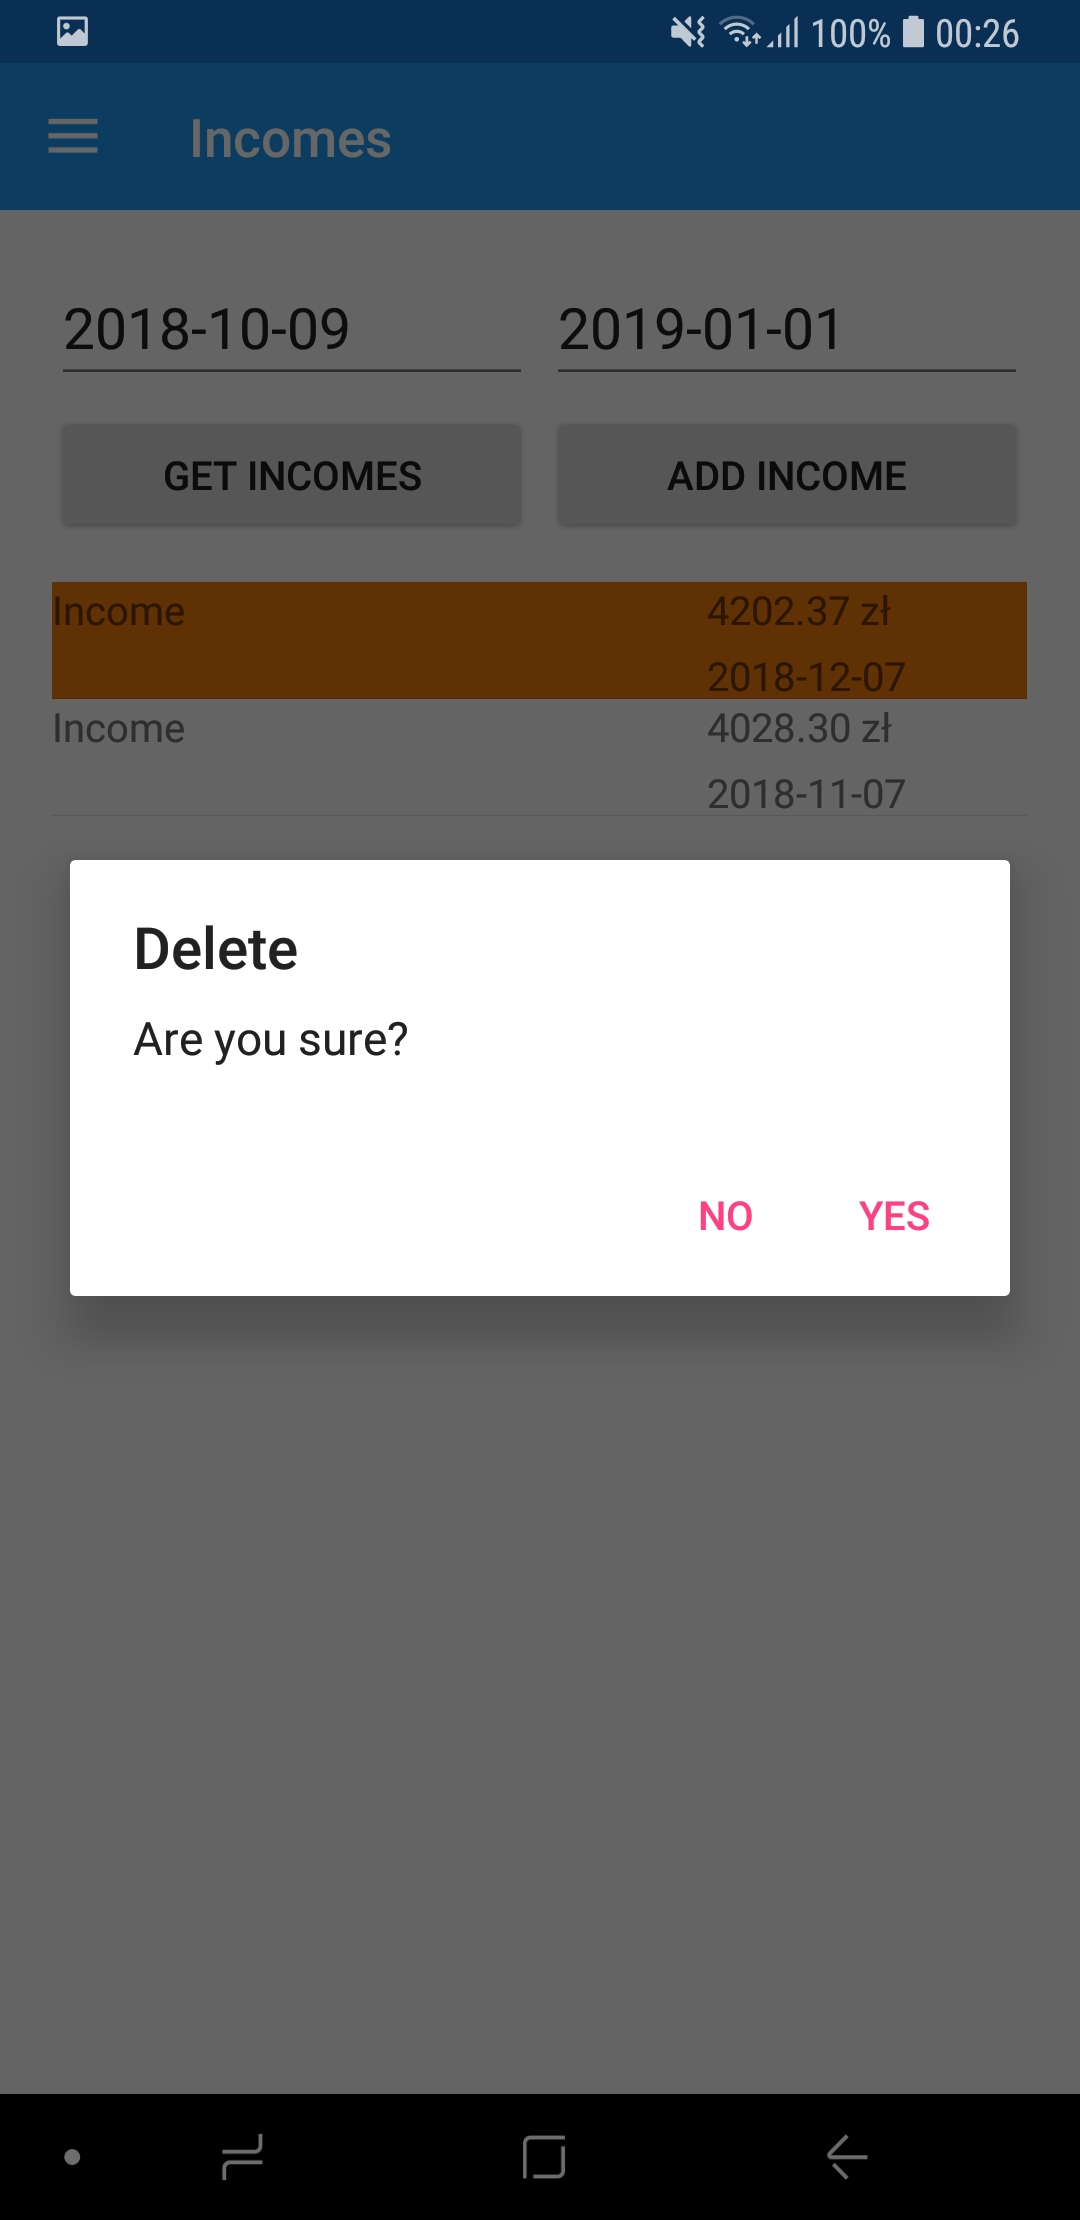
\includegraphics[width=1.75in]{img/mobile/usun_na_pewno.jpg}
			\subcaption{Okno potwierdzające chęć usunięcia przychodu.}
			\label{usun_na_pewno}
		\end{subfigure}
	\end{center}
	\caption{Zrzuty ekranu procesu usuwania przychodu.}
\end{figure}


\section{Moduł rejestracji wydatków}
W zakres modułu rejestracji wydatków wchodzą następujące przypadki użycia:
\begin{itemize}
	\item wyświetl swoje wydatki,
	\item dodaj wydatek,
	\item edytuj wydatek,
	\item usuń wydatek,
	\item wykonaj predykcję wydatków.
\end{itemize}

Operacje wyświetlania, dodawania, edycji oraz usuwania wydatków wykonuje się analogicznie do ich odpowiedników z modułu rejestracji przychodów.

\textbf{Predykcja wydatków} (przypadek użycia "wykonaj predykcję wydatków") jest to wykonanie prognozy wydatków powiązanych z wydatkiem głównym na nadchodzące miesiące. Po wybraniu z menu bocznego (Rys. \ref{hamburger_predykcja}) strony "Prediction" (Rys. \ref{predykcja}), uzupełnieniu wartości, daty oraz kategorii wydatku i naciśnięcie przycisku "PREDICTION" użytkownik otrzymuje prognozę wydatków na trzy nadchodzące miesiące (Rys. \ref{predykcja_gotowe}).
\begin{figure}[!ht]
	\begin{center}
		\begin{subfigure}[b]{0.3\textwidth}
			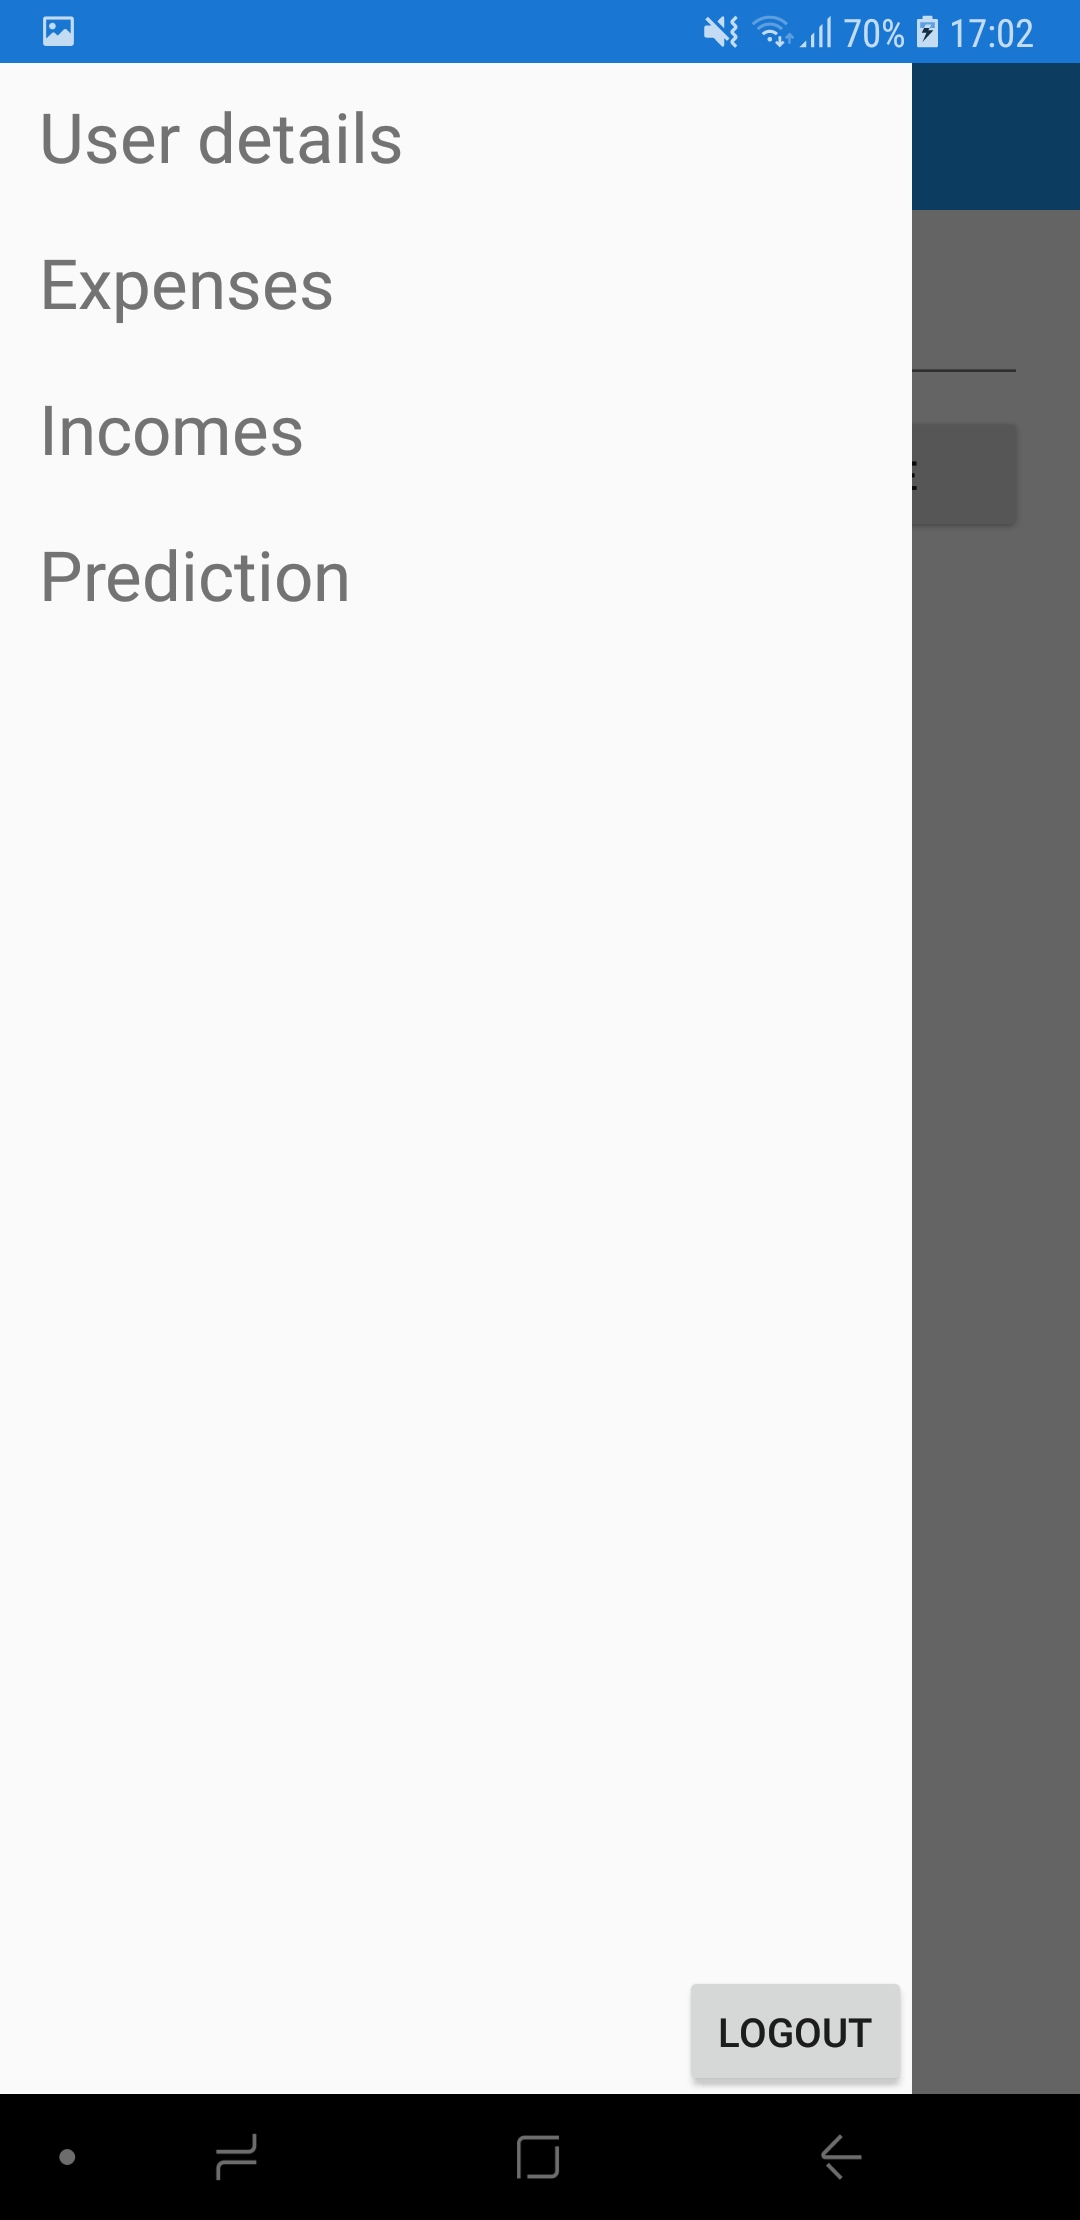
\includegraphics[width=1.75in]{img/mobile/menu_boczne.jpg}
			\subcaption{Menu boczne.}
			\label{hamburger_predykcja}
		\end{subfigure}
		\begin{subfigure}[b]{0.3\textwidth}
			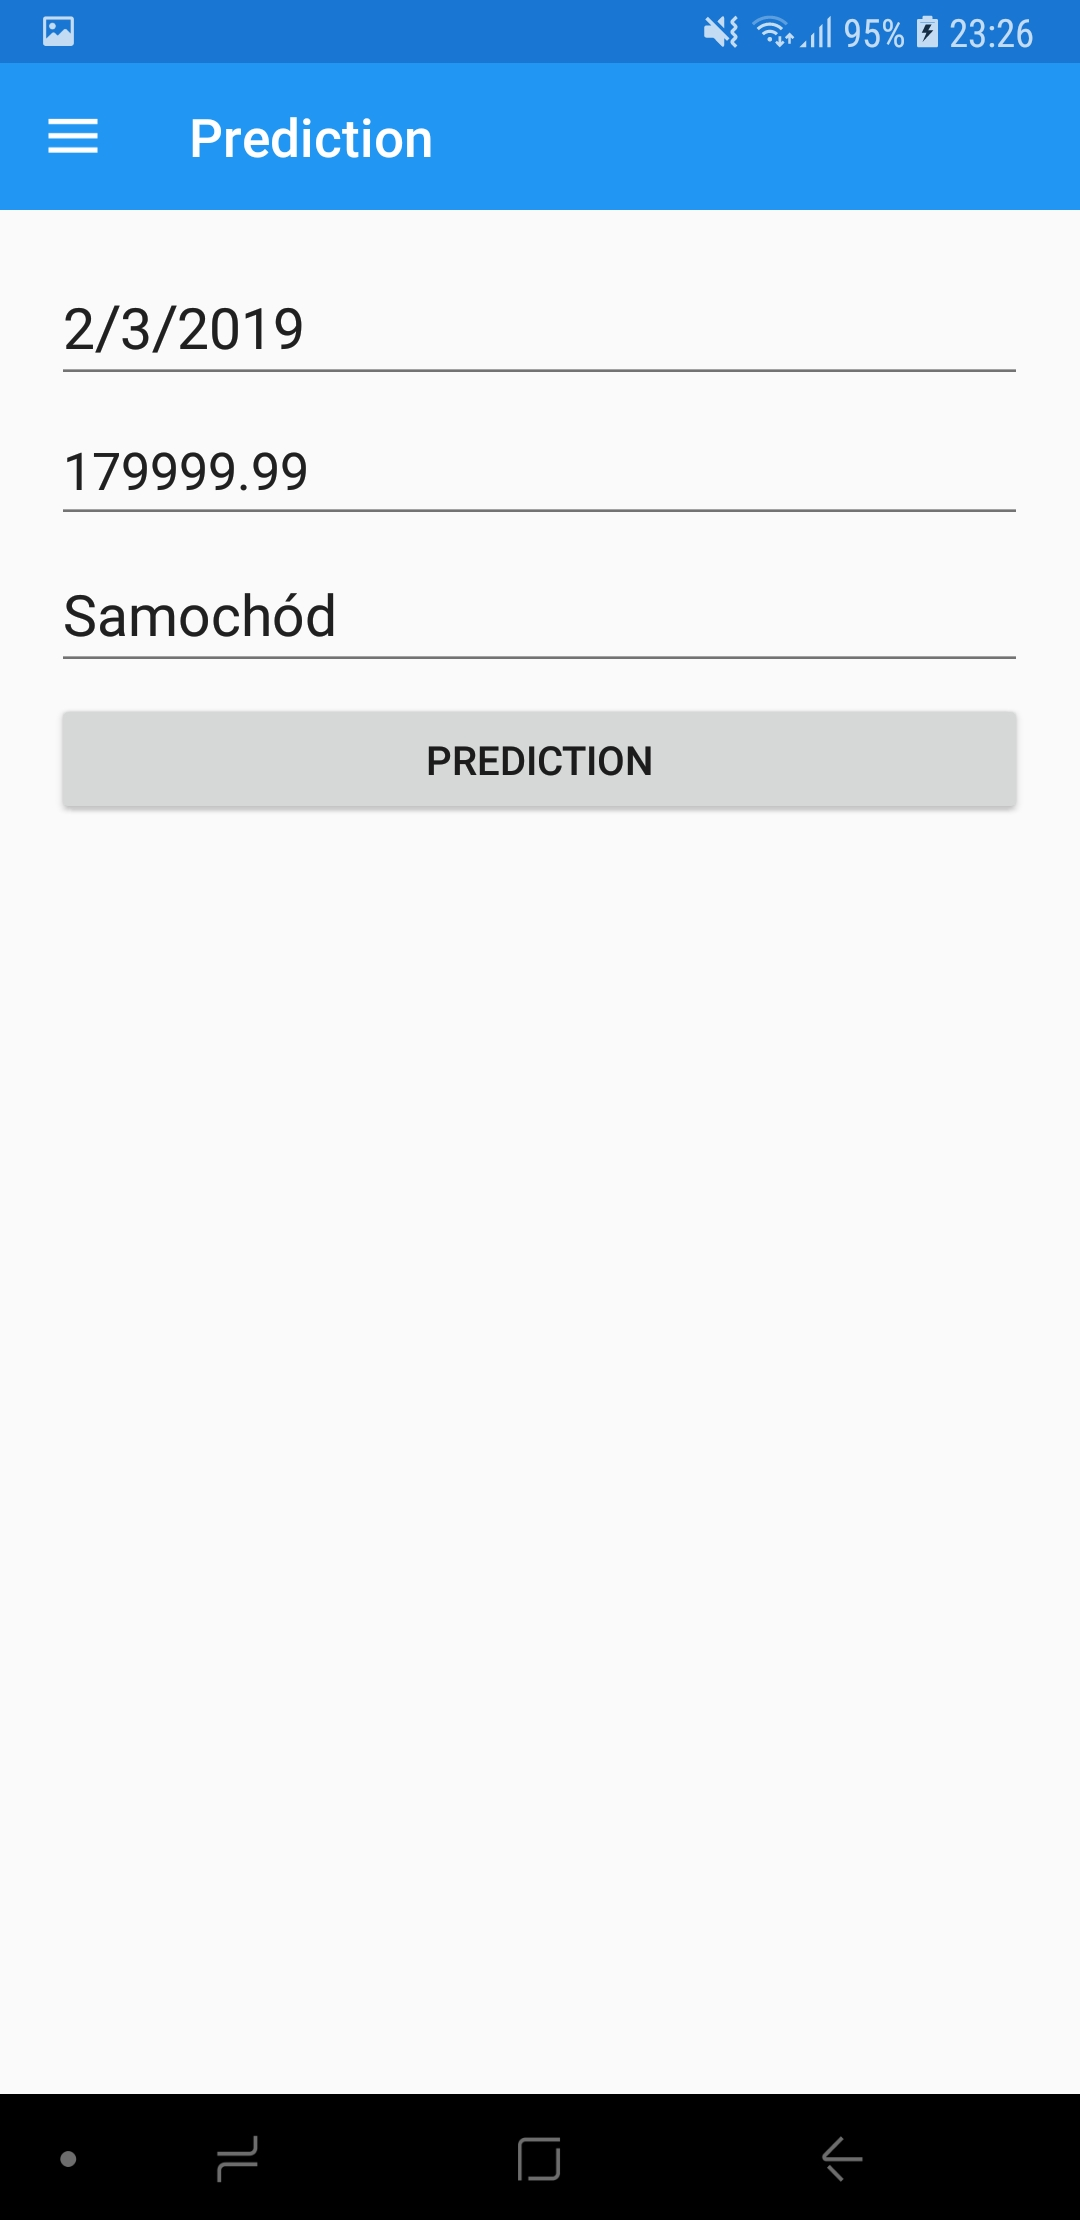
\includegraphics[width=1.75in]{img/mobile/predykcja.jpg}
			\subcaption{Strona predykcji.}
			\label{predykcja}
		\end{subfigure}
		\begin{subfigure}[b]{0.3\textwidth}
			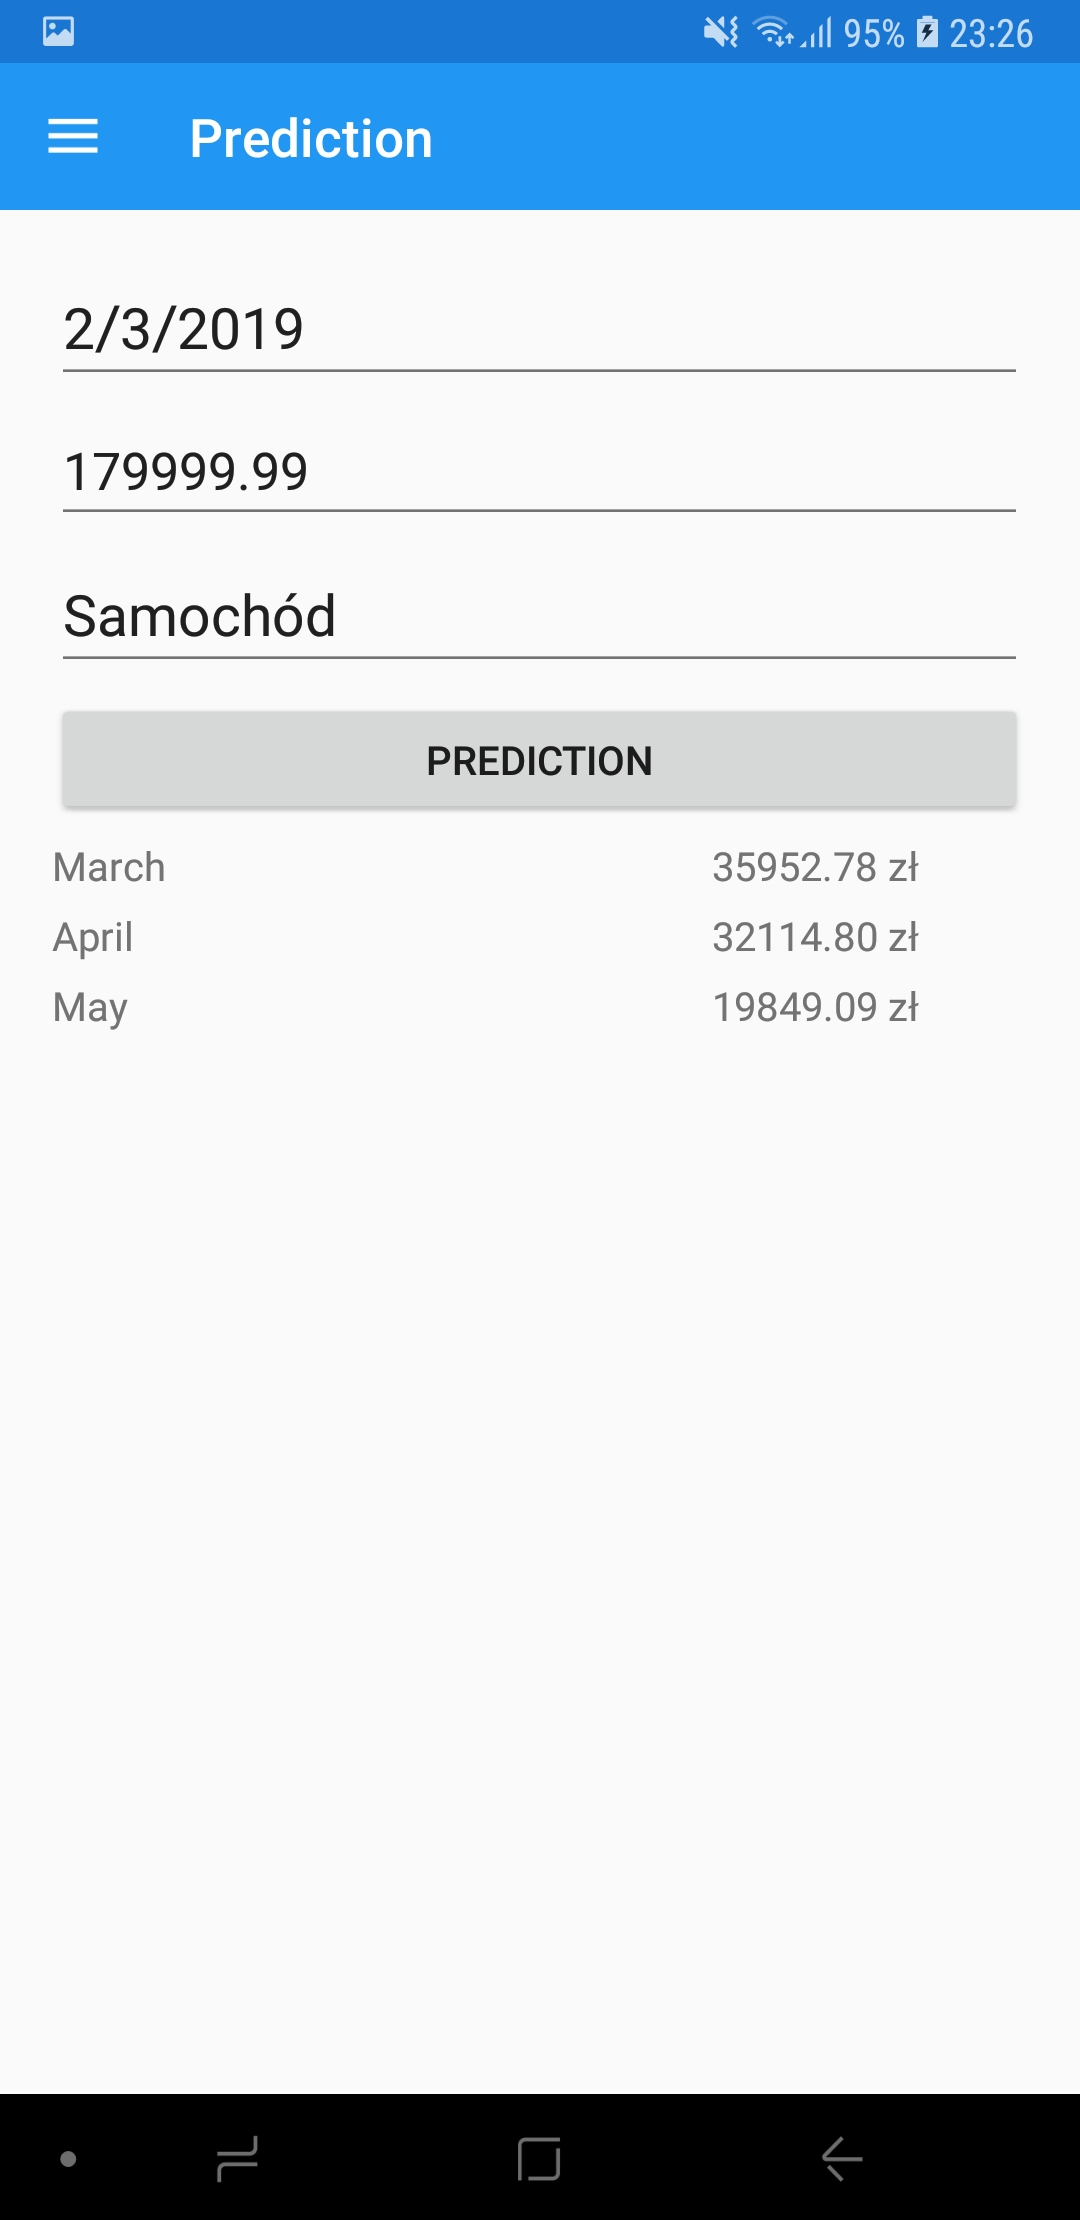
\includegraphics[width=1.75in]{img/mobile/predykcja_gotowe.jpg}
			\subcaption{Wyniki predykcji.}
			\label{predykcja_gotowe}
		\end{subfigure}
	\end{center}
	\caption{Zrzuty ekranu procesu wykonywania predykcji wydatków.}
\end{figure}
\chapter{Podsumowanie}
\section{Wnioski}
\section{Perspektywy rozwoju}
\bibliographystyle{ieeetr}
\bibliography{sample.bib}
\listoffigures
%\listoftables
\lstlistoflistings
\end{document}